\documentclass[a4paper]{report}
\usepackage[utf8]{inputenc}
\DeclareUnicodeCharacter{2010}{-}% support older LaTeX versions
\usepackage{hyperref}
\usepackage{amsmath}
\usepackage{tikz}
\usepackage{tikz-qtree}
%\usepackage{subfigure}
\usepackage{graphicx}
\usepackage[numbers]{natbib}

% paper1
\usepackage{amsthm,amssymb,amsfonts}
\usepackage{xspace}
\usepackage{enumitem}
\usepackage{algorithm}
\usepackage{algorithmicx}
\usepackage[noend]{algpseudocode}
\usepackage{algpseudocode}
\usepackage{parskip}
\usepackage{subcaption}
%\usepackage{subfig}
\usepackage{multirow}
\usepackage{adjustbox}

%% paragraph
%\usepackage{titlesec}
\setcounter{secnumdepth}{4}


\graphicspath{
	{./figs/}
}

\hypersetup{letterpaper,bookmarksopen,bookmarksnumbered,
pdfpagemode=UseOutlines,
colorlinks=true,
linkcolor=blue,
anchorcolor=blue,
citecolor=blue,
filecolor=blue,
menucolor=blue,
urlcolor=blue
}

\DeclareMathOperator*{\argmax}{arg\,max}

%opening
\title{Provably Constant-time Motion Planning}
\author{Fahad Islam\\
The Robotics Institute\\
Carnegie Mellon University\\
\texttt{fi@andrew.cmu.edu}
\\
\\
\Large{Thesis Proposal}\\
\\
\\
\\
\\
\\
\vspace{2mm}
\textbf{Thesis Committee:}\\
Maxim Likhachev (Chair)\\
Chris Atkeson\\
Oliver Kroemer\\
Siddhartha Srinivasa (UW)\\
Oren Salzman (Technion)\\
\\
\\
\textit{Submitted in partial fulfillment of the requirements
for the degree of}\\
\textit{Doctor of Philosophy in Robotics.}\\
\\
\\
Copyright~$\copyright$ 2020 Fahad Islam. All rights reserved.
}

\newtheorem{theorem}{Theorem}
\newtheorem{lemma}{Lemma}
%\newtheorem{definition}{Definition}
%\newtheorem{cor}{Corollary}

%\newcommand{\calX}{\ensuremath{\mathcal{X}}\xspace}
%\newcommand{\calL}{\ensuremath{\mathcal{L}}\xspace}
%\newcommand{\calS}{\ensuremath{\mathcal{S}}\xspace}
%\newcommand{\calR}{\ensuremath{\mathcal{R}}\xspace}
%\newcommand{\calD}{\ensuremath{\mathcal{D}}\xspace}
%\newcommand{\calP}{\ensuremath{\mathcal{P}}\xspace}

\newcommand{\sAttract}{\ensuremath{s^{\text{attractor}}_i}\xspace}
\newcommand{\sStart}{\ensuremath{s_{\text{start}}\xspace}}
\newcommand{\sGoal}{\ensuremath{s_{\text{goal}}\xspace}}
\newcommand{\sNom}{\ensuremath{s_{\text{nominal}}\xspace}}
\DeclareMathOperator*{\argmin}{arg\,min}
% Caligraphic letters:
\newcommand{\calA}{\ensuremath{\mathcal{A}}\xspace}
\newcommand{\calC}{\ensuremath{\mathcal{C}}\xspace}
\newcommand{\calE}{\ensuremath{\mathcal{E}}\xspace}
\newcommand{\calG}{\ensuremath{\mathcal{G}}\xspace}
\newcommand{\calR}{\ensuremath{\mathcal{R}}\xspace}
\newcommand{\calM}{\ensuremath{\mathcal{M}}\xspace}
\newcommand{\calN}{\ensuremath{\mathcal{N}}\xspace}
\newcommand{\calX}{\ensuremath{\mathcal{X}}\xspace}
\newcommand{\calS}{\ensuremath{\mathcal{S}}\xspace}
\newcommand{\calQ}{\ensuremath{\mathcal{Q}}\xspace}
\newcommand{\calT}{\ensuremath{\mathcal{T}}\xspace}
\newcommand{\calL}{\ensuremath{\mathcal{L}}\xspace}
\newcommand{\calB}{\ensuremath{\mathcal{B}}\xspace}
\newcommand{\calW}{\ensuremath{\mathcal{W}}\xspace}
\newcommand{\calV}{\ensuremath{\mathcal{V}}\xspace}
\newcommand{\calP}{\ensuremath{\mathcal{P}}\xspace}
\newcommand{\calD}{\ensuremath{\mathcal{D}}\xspace}
\newcommand{\calF}{\ensuremath{\mathcal{F}}\xspace}
\newcommand{\calO}{\ensuremath{\mathcal{O}}\xspace}


% math
\newcommand{\R}{\mathbb{R}}
\newcommand{\Z}{\mathbb{Z}}
\newcommand{\A}{\mathbb{A}}
\newcommand{\N}{\mathbb{N}}
\newcommand{\Q}{\mathbb{Q}}
\newcommand{\C}{\mathbb{C}}
\newcommand{\K}{\mathbb{K}}

% Motion planning
\newcommand{\Sgoal}{\ensuremath{S_{\rm goal}}\xspace}
\newcommand{\Cfree}{\ensuremath{\calC_{\rm free}}\xspace}
\newcommand{\Cobs}{\ensuremath{\calC_{\rm obs}}\xspace}
\newcommand{\Cforb}{\ensuremath{\calX_{\rm forb}}\xspace}
%\newcommand{\Csafe}{\ensuremath{\calX_{\rm free}^{\rm safe}}\xspace}
\newcommand{\Cspace}{\calC-space\xspace}

% =
\newcommand{\eg}{{e.g.,}\xspace}
\newcommand{\ie}{{i.e.,}\xspace}
\newcommand{\etc}{{etc.}\xspace}
\newcommand{\etal}{{et~al.}\xspace}

\def\naive{{na\"{\i}ve}\xspace}

\def\OS#1{\textcolor{magenta}{#1}}
\def\FI#1{\textcolor{cyan}{#1}}

\newtheorem{thm}{Theorem}
\newtheorem{lem}{Lemma}
%\newtheorem{thm}{Theorem}[section]
\newtheorem{observation}[thm]{Observation}
%\newtheorem{thm}{Theorem}
\newtheorem{cor}{Corollary}
\newtheorem{definition}[thm]{Definition}


%tex tools
\newcommand{\ignore}[1]{}
\newcommand{\first}[2]{#1}
\newcommand{\second}[2]{#2}
\newcommand{\arxiv}[2]{#2}


\newcommand\algname[1]{\textsf{#1}\xspace}
\newcommand\astar{\algname{A*}}
\newcommand\rrt{\algname{RRT}}
\newcommand\wastar{\algname{wA*}}


%paper-related macros
\newcommand\Gfull{\ensuremath{G^{\textrm{full}}}\xspace}
\newcommand\Gcov{\ensuremath{G^{\textrm{cov}}}\xspace}
\newcommand\Guncov{\ensuremath{G^{\textrm{uncov}}}\xspace}
\newcommand\Gcovp{\ensuremath{G'^{\textrm{cov}}}\xspace}
\newcommand\Guncovp{\ensuremath{G'^{\textrm{uncov}}}\xspace}
\newcommand\Shome{\ensuremath{s_{\textrm{home}}}\xspace}
\newcommand\Tbound{\ensuremath{T_{\textrm{bound}}}\xspace}
\newcommand\Trc{\ensuremath{t_{\textrm{rc}}}\xspace}
\newcommand\Ssc{\ensuremath{s_{\textrm{sc}}}\xspace}
\newcommand\Sstart{\ensuremath{s_{\textrm{start}}}\xspace}
\newcommand\Xexec{\ensuremath{x_{\textrm{exec}}}\xspace}

%comments
\def\os#1{\textcolor{magenta}{#1}}
\def\fis#1{\textcolor{red}{#1}}
\def\bound#1{\textcolor{blue}{#1}}

\def\AlgFontSize{\small}
\def\CaptionTextSize{\small}
\begin{document}

\maketitle

%\begin{center}
%\Large{Thesis Proposal}
%\vspace{40mm}
%
%\large{
%\textbf{Thesis Committee:}
%
%Maxim Likhachev (Chair)\\
%Chris Atkeson\\
%Oliver Kroemer\\
%Siddhartha Srinivasa (UW)\\
%Oren Salzman (Technion)\\
%}
%
%\vspace{10mm}
%\textit{Submitted in partial fulfillment of the requirements
%for the degree of Doctor of Philosophy in Robotics.}
%
%\vspace{10mm}
%Copyright~$\copyright$ 2020 Fahad Islam. All rights reserved.
%\end{center}
%\newpage

\begin{abstract}
In manufacturing and warehouse scenarios, robots often perform recurring manipulation tasks in structured environments. Fast and reliable motion planning is one of the key elements that ensure efficient operations in such environments. A very common example scenario is of manipulators working at conveyor belts, where they have limited time to pick moving objects and if the planner exceeds a certain time threshold, they would fail to pick the objects up. Similar scenarios are encountered in automated assembly lines. Such time-critical applications spur the need for planners which are \emph{guaranteed} to be fast. To this end we introduce and formalize the concept of Constant-time Motion Planning (CTMP); namely, the ability to provably guarantee to generate a motion plan within a (small) constant time. We then develop several algorithms that fall into the class of CTMP algorithms.

Specifically, up to now we have developed constant-time motion planning algorithms for two domains; (1) Manipulation for repetitive tasks in static environments (2) Manipulation for the task of picking up moving objects (of known models) off a conveyor belt. For the latter, the robot typically perceives a rough pose estimate viewing from a distance, but it must start moving early on (relying on that rough estimate) to be able to reach the object in time and then adjust its motion in real time as it gets improved estimates.
Our key insight is that since these domains are fairly repetitive, the space in which the robot operates is a very small subset of its configuration space, which allows us to preprocess it exhaustively. The preprocessing step generates a representative set of paths that can be used by search at query time in a way that assures small constant-time planning.
%
For the former domain, we evaluate our algorithm for a mail sorting task in simulation on PR2 and also test the algorithm on a real truck-unloading robot. For the latter domain, we perform real robot experiments on PR2 working at a conveyor belt.

For the remainder of this thesis we propose the following work. First, we propose to further study and formalize what CTMP implies in practice and what underlying assumptions it entails. Second, we propose to extend our  planning framework to semi-static environments (i.e. containing some movable obstacles). Third, we aim to boost the capability of the conveyor pick-up task by having multiple robot arms simultaneously picking up objects, while still maintaining constant-time planning guarantees.

%For the remainder of this thesis we propose the following work. First, we propose to further study and formally define what constant-time planning implies in practice and what underlying assumptions it entails. Second, we propose to extend our  planning framework to semi-static environments (containting some movable obstacles). Third, we aim to boost the capability of the conveyor pick-up task by having multiple robot arms simultaneously picking up objects, while still maintaining strong theoretical guarantees on the planning side.
%This introduces new algorithmic challenges including decision making about which object to assign to which arm and motion synchronization between the arms.
\end{abstract}
\newpage

\tableofcontents
\newpage

\chapter{Introduction}
\section{Motivation}
In industrial settings such as manufacturing and warehouse environments, the robots typically operate in structured environments and perform repetitive tasks. Despite significant advancements in the field of motion planning in the past several decades, a large percentage of warehousing and manufacturing industry still uses robots that run hardcoded routines to perform very specific tasks. The lack of penetration of modern motion planning algorithms at scale can be attributed to the fact that the industry needs systems which are \emph{guaranteed} to be fast and reliable, even at the cost of flexibility that these systems could potentially provide.

In warehouses, robots are widely deployed at fast moving conveyor belts to perform repetitive pick and place or sorting tasks, which gives them a very short time budget to plan their motion. Failing to plan within that time, a robot would skip objects and affect the throughput of the system. Similarly in assembly lines where multiple robots operate in their respective work stations, an overhead caused by the motion planner at one station can slow down the entire chain. This thesis focuses on such time critical applications and introduces the notion of (small) Constant-time Motion Planning (CTMP). CTMP implies generating motion plans in provably-bounded short planning times.

This thesis is motivated by the following key observations from the aforementioned domains; (1) The tasks are highly repetitious (2) The  environments are fairly structured. (1) gives us an insight that the operational space of the robot is a very small as compared to its full C-space and (2) implies that the environment model is known in advance. These two aspects allow us to fully preprocess the part of the C-space that the robot operates in while accounting for the known objects that exist in its surroundings.

A naive way of providing constant-time guarantees would be to precompute paths for all possible start and goal states that the planner could be queried for and use a simple hash lookup at query time (assuming the lookup time is constant). However, as the set of start or goal states increase, this approach quickly becomes intractable, memory and precomputation time-wise. Our method provides a compression scheme and precomputes only a small set of representative paths which can still ``cover" the robot's operational space. Namely, using this set of paths, at query time, our method can solve any query within the robot's operational space in constant time.

\section{Approach}
\label{sec:approach}
So far, we have developed CTMP algorithms for two domains.
\subsection{Manipulation for repetitive tasks in static environments}
In this work, we consider the specific case where the start state is fixed and there exists a ``goal region" which contains all possible goals. Consider for example, a typical mailroom scenario where the robot has to pick up mail from a fixed location and sort them in cubby shelves. The start corresponds to the pickup location for the packages and the goal region corresponds to all possible goal poses within the cubby shelves. Note that the cubbies reduce the robot's operational space drastically which makes the preprocessing tractable for our method.

Our key insight is that given an ``attractor state'' in the goal region, typically there is a large region of states around it for which a greedy search (a search following an attractive potential function) towards the attractor state is collision free. We show that such so called ``attractor regions" can be efficiently computed by using dynamic programming.
Importantly, the runtime-complexity of such a greedy search is bounded and there is no need to perform computationally-complex collision-detection operations. 
This insight allows us to generate in an offline phase a small set of these attractor regions together with a path between each attractor state and the start, ensuring that together these attractor regions completely cover the full goal region.
In the query phase, a path is generated by performing a greedy search from the goal to an attractor state (the one which contains the goal) followed by the precomputed path from the start. The approach is described in detail in chapter~\ref{chap:icaps}.

\subsection{Manipulation for picking up moving objects off a conveyor belt}
In this domain, the robot's task is to reliably and safely pickup objects coming on a conveyor belt. We will refer to this problem as ``conveyor-pickup task". We assume that the geometric models of the target objects are known in advance. The success of manipulation tasks relies heavily on the accuracy of the perception system which often is noisy, especially if the target objects are perceived from a distance. For fast moving conveyor belts, the robot cannot wait for a perfect estimate before it starts execution. In order to be able to reach the object in time it must start moving early on (relying on the initial noisy estimates) and adjust its motion on-the-fly in response to the pose updates from perception. We developed an approach that meets these requirements by providing provable constant-time planning and replanning guarantees.

Again, with the same insight, in the first step we precompute a small set of paths from a fixed start (say drop off location) that can cover the goal region which in this domain is defined in the space of object poses. The goal can be any arbitrary object pose~$(x,y,yaw)$ of the objects. In the second step, we uniformly discretize these paths in time to get a set of states that we call ``replannable'' states. To handle pose updates online, we may need to replan from any of these states to all the goals in the goal region. The algorithm then goes back to the first step treating all the replannable states as new starts and this recursive process continues until all replannable states are taken care of. While the approach has exponential complexity in the number of timesteps from the start to the goal, we drastically save on computation and memory by reusing the first set of paths (from the drop off location to the goal region). Our algorithm guarantees that for any replannable state and a goal, a plan is be computed in constant time. Experimentally we observe that the robot fails most of the time without replanning i.e. in case it relies on the first estimate or if it waits for an accurate estimate before starting planning. The details of the framework is provided in chapter~\ref{chap:rss}.

\subsection{Manipulation for repetitive tasks in semi-static environments}
In many applications, including logistics and manufacturing, robot manipulators operate in semi-static environments alongside humans or other robots. These environments are largely static, but they may contain some movable obstacles that the robot must avoid. Manipulation tasks in these applications are often highly repetitive, but require fast and reliable motion planning capabilities, often under strict time constraints. Existing preprocessing-based approaches are beneficial when the environments are highly-structured, but their performance degrades in the presence of movable obstacles, since these are not modelled a priori.

We propose a novel preprocessing-based method called Alternative Paths Planner (APP) that provides provably fixed-time planning guarantees in semi-structured environments. Our key insight is that for a given start and goal, a small number of \emph{disjoint} alternative paths would suffice for any configuration of the movable obstacles. APP attempts to plan a set of such alternative paths offline such that, for any configuration of the movable obstacles, at least one of the paths from this set is collision-free. During online execution, a collision-free path can be looked up efficiently within a few microseconds. 

\subsection{Manipulation for protecting against attacks using a shield}

\section{Expected Contribution}
To summarize, we make the following contributions in this thesis.
\begin{itemize}
	\item Introduce and formalize the concept of Constant-time Motion Planning (CTMP)
	\item Develop CTMP algorithm for domains with repetitive manipulation tasks in static environments
	\item Develop CTMP algorithm for the conveyor-pickup task
	\item Develop CTMP algorithm for domains with repetitive manipulation tasks in semi-static environments
	\item Develop CTMP algorithm for robot-shielding task
\end{itemize}

\newpage
\chapter{Background}
\section{Configuration Space and Motion Planning}
Motion planning algorithms operate in the state space often also referred to as the \emph{configuration space} (C-space) or~$\calC$~\cite{lozano1990spatial}. In this space a state or a configuration of the robot can be uniquely represented as a point which makes it convenient for the motion planners to operate. It can be the~($x,y$) position of the robot or~($x,y,yaw$) if the orientation also matters. For a robot arm the configuration can be composed of all the joint positions. If planning with dynamics, the velocities and times may also be added to the configuration. Similarly higher order derivatives can also be added as per the requirements of the domain. The number of variables in the configuration represents the \emph{dimension} of the C-space. For example, for a 7DoF robot arm, for only considering the joint positions, the dimension of the C-space is seven. The free space~$\Cfree$ contains all the configurations which are valid with respect to some state validity criterion such as violation of obstacle collision constraints or kinematic constraints etc. The obstacle space~$\Cobs$ contains all the configurations which are invalid and so~$\Cobs = \calC \backslash \Cfree$.

For the general motion planning problem we define a start configuration~$\Sstart$ and a goal set~$\Sgoal$. The goal can be under-specified as the pose of the robot end-effector or the pose of the target object. For instance, given a target object that the robot needs to grasp, the goal can be the grasp pose (i.e. position and orientation of the end-effector) or it can be even more under-specified as the pose of the object, giving the flexiblity to select different grasp poses. The motion planning problem is defined as finding a continuous path~$\tau : [0:1] \rightarrow \Cfree$ s.t. $\tau(0) = \Sstart$ and $\tau(1) \in \Sgoal $. Typically in practice most motion planning algorithms find a path of the form~$[s_0, s_1, s_2,...,s_n] \in \Cfree$ s.t. $s_0 = \Sstart$ and $s_n \in \Sgoal$ assuming that the consecutive states i.e $s_i, s_{i+1}$ can be connected via some simple interpolation scheme.

Computing~$\Cfree$ is extremely hard, specially in higher dimensions. Instead of doing that, most motion planners generally sample in~$\Cfree$ and use a collision checker to identify the validity of a configuration. These planners typically sample states in~$\Cfree$ using rejection sampling, connect those samples to construct a graph (or a tree) and then use graph search to find the path from a start to goal. These algorithms are called sampling-based algorithms. A motion planner is referred to as \emph{complete} if it guarantees to find a path if one exists, and otherwise returns failure. Sampling-based planners are \emph{probablisitically complete}, meaning that in the limit of the number of samples they are guaranteed to find a solution if one exists.

\section{C-space representation for Search-based Planning}
\label{sec:sbp}
Search-based planning methods discretize the C-space into cells. This discretization generally relies on a grid-based or lattice-based structure. A cell is the smallest unit of this discrete space and represents a small volume of C-space states that lie within it. A representative state within a cell, commonly its geometric center is picked to denote a vertex for that cell. All the vertices~$\calV$ connect to their neighboring vertices through edges~$\calE$ to construct a graph~$\calG = (\calV, \calE)$. These edges may have associated costs. Only those vertices and edges are added to~$\calG$ that are valid. The motion planning problem is thus turned into a graph search problem which can be solved using any graph search algorithm. The search is done on an implicit graph as opposed to explicit graph. Namely, instead of precomputing the entire graph which is infeasible for large domains, the graph is constructed and evaluated on-the-fly as the search progresses.

The C-space discretization is done at a certain resolution which is a domain dependent parameter. The resolution determines how course or fine the discretization is. Search-based algorithms are attributed as \emph{resolution complete} which means that they will return a path if one exists for the given resolution. Note that it is possible that a solution exists in the C-space and the search-based planner fails to find it because the resolution is not fine enough for that problem.

\section{Computational Complexity in Motion Planning}
The general motion planning problem was shown by Reif to be PSPACE-hard~\cite{reif1979complexity}. Later it was shown to be PSPACE-complete by Canny~\cite{canny1988complexity}. Their analysis was based on finding the \emph{exact} solutions. The class of algorithms that go for finding the exact solutions are called combinatorial algorithms or \emph{exact} algorithms~\cite{lavalle2006planning}. These algorithms do not rely on any approximation of the C-space and guarantee completeness for the exact motion planning problem.

The dimension~$d$ of the C-space is the most crucial element in determining the complexity of the motion planning problem. It has been shown that for the general motion planning problem the computational complexity grows exponentially with~$d$~\cite{chazelle1991singly}.

The exact motion planning algorithms do not scale to more complex problems as they make certain limiting assumptions about the geometry of the robot and the obstacles. In contrast, the modern approaches use approximations of the general motion planning problem by relaxing the completeness guarantees. For example the sampling-based algorithms approximate the problem structure via random sampling in the C-space and so they relax the completeness guarantee to probabilistic completeness. Search-based algorithms approximate the problem via space discretization with a certain resolution, hence they are resolution complete.
Since the exact methods are no more used in modern days, the computational complexity analysis for the general motion planning problem is of less relevance now and the analysis for the approximate methods is based on the underlying approximation. For instance, for sampling-based methods the complexity is analysed in the number of samples and for search-based methods it is analysed in the size of the grid or the lattice structure.


\newpage
\chapter{Related Work}
\label{sec:rel}
Our approach leverages preprocessing in order to speed up online planning. In this respect, first we cover some popular preprocessing-based approaches. Second, we review techniques that reuse previously generated plans or experiences to accelerate planning. Our method also bears resemblence with these methods as it also uses paths that are generated in the preprocessing phase during online planning. Third, we cover real-time planning methods as they provide constant-time guarantees for limited-horizon planning, the property that our approach also offers, while highlighting the key differences. We then review some work from the controls communitee that explored similar concepts that our method builds upon. Finally, we cover some of the motion planning approaches that are particularly related to the conveyor-pickup task.

\section{Preprocessing-based Methods}
Preprocessing-based motion planners often prove beneficial for real-time planning. They analyse the configuration space offline to generate some auxiliary information that can be used online to speed up planning. 

The most reknowned example is the Probablistic Roadmap Method (PRM)~\cite{kavraki1996probabilistic}. They have a preprocessing and a query phase. In the preprocessing phase a roadmap is constructed in $\Cfree$ by randomly sampling valid states in the C-space and connecting them to their neighboring states if the edges making the connections are valid. In the query phase the start and goal states are connected to their neighboring states in the roadmap (if valid connections are possible) and then any search algorithm like A* search is used to find the path. PRM methods are categorized as multi-query methods meaning that once the roadmap is constructed it can be used to answer multiple queries for the same environment. Query times can be significantly sped up by further preprocessing the roadmaps using landmarks~\cite{paden2017landmark}. Recently,the repetition roadmap~\cite{LA18} was suggested as a way to extend the PRM for the case of multiple highly-similar scenarios. Some of these methods have been integrated with sparse motion-planning roadmaps (see e.g.,~\cite{SSAH14,DB14}) to reduce the memory footprint of the algorithm. All these methods only provide probablistic completeness guarantees.

Our work bares resemblance to previous work on 
subgoal graphs~\cite{UK17,UK18}.
Subgoal graphs is a search-based method that preprocesses the entire C-space to generate a sparse overlay graph comprised of vertices called sub-goals. The pair of sub-goals connected by an edge are \emph{reachable} and thus searching on this overlay graph is significantly faster than searching on the original graph. The method assures that the path found on this subgoal graph has a path on the original graph and can be quickly computed at query time. As this method requires preprocessing the full C-space it is expensive and only is applicable to lower dimensional planning problems.

While all these preprocessing-based approaches speedup planning times compared to planning from scratch by using the preprocessed information, they do not provide constant-time bounds on the planning times.

\section{Motion Planning with Reuse}
An effective approach to speed up planning is to precompute a set of complete paths into a library and given a query, attempt to match complete paths from the library to the new query~\cite{berenson2012robot,jetchev2013fast}.
Using paths from previous search episodes (also known as using experience) has also been an active line of work~\cite{PCCL12,PDCL13,BAG12,CSMOC15}. E-graphs method~\cite{PCCL12} computes a heuristic function to guide the search in such a way as to reuse search efforts from previously generated paths. The Lightning framework~\cite{BAG12} runs two modules in parallel, a module that runs the planner from scratch and a module that retrieves and repairs path stored in a library. The Thunder framework~\cite{CSMOC15} also leverages previous experiences and the experiences are generated using probabilistic sampling. The experiences are stored as sparse roadmap spanner~(SPARS). 

These methods also provide significant speedups in planning times. Our method borrows some techniques from these methods but in a way by which we can provide constant-time planning guarantees which these algorithms do not offer.

\section{Real-time Motion Planning}
\label{rel:real}
There is a family of real-time search algorithms that provide constant-time guarantees~\cite{KL06,KS09,K90,bjornsson2009tba}.
	To provide guarantees on planning time the search only looks at a finite horizon, generating a partial plan, and interleaves planning and execution. In planning cycles, the robot may re-expand states multiple times. In addition, during execution, the robot is likely to visit the same states multiple times before it reaches the goal which can result in highly suboptimal behavior specially in higher dimensional problems. These algorithms run repeated A* searches and update the heuristic values in the local search spaces while maintaining the admissibility of the heuristics. The heuristics get more informed as the search is run repeatedly. By doing so they provide completeness guarantees, meaning that the robot will eventually arrive at the goal.

In contrast to these algorithms, our methods either plan for indefinite horizons i.e. all the way from the start to the goal while providing constant-time planning guarantees or do limited horizon planning (interleaving planning and execution) in constant-time while assuring that the executed path, if reconstructed would not contain any cycle.

Artificial potential field methods can also be used for real-time behavior~\cite{warren1989global,vadakkepat2000evolutionary}. However these methods are incomplete and can get trapped in local minima.

\section{Global Control using Local Potential Functions}
Finally, our notion of ``attractor regions" which we touched upon in section~\ref{sec:approach}, is similar (in spirit) to control-based methods that  ensure safe operation over local regions of the free configuration space~\cite{CRC03,CCR06,tedrake2010lqr}. Metaphorically they name these regions as ``funnels" that collapse a large set of input conditions to a single policy.
These regions are then used within a high-level motion planner to compute collision-free trajectories. For instance, LQR-trees~\cite{tedrake2010lqr} computes local stability regions to build a sparse tree of LQR-stabilized trajectories. The union of these local regions covers the entire state space ensuring that all initial conditions that are capable of reaching the goal will reach the goal.


\section{Motion Planning for Conveyor-pickup Task}
Existing work on picking moving objects has focused on different aspects of the problem ranging from closed-loop controls to object perception and pose estimation, motion planning and others~\cite{allen1993automated, han2019toward, stogl2017tracking, zhang2018gilbreth}. 
%
Here, we focus on motion-planning related work. Time-configuration space representation was introduced to avoid moving obstacles~\cite{fraichard1993dynamic,cefalo2013task,yang2018planning}. Specifically in ~\cite{yang2018planning}, a bidirectional sampling-based method with a time-configuration space representation was used to plan motions in dynamic environments to pickup moving objects. While their method showed real-time performance in complex tasks, it used fully specified goals which weakens the completeness guarantees. Furthermore their method is probablistically complete and therefore, does not offer provable real-time behavior. Graph-search-based approaches have also been used for the motion-planning problem of the conveyor-pickup task~\cite{cowley2013perception, menon2014motion}. The former uses a kinodynamic motion planner to smoothly pick up moving objects i.e., without an impactful contact. A heuristic search-based motion planner that plans with dynamics and could generate optimal trajectories with respect to the time of execution was used. While this planner provides strong optimality guarantees, it is not real-time and thus cannot be used online.
%
The latter work was demonstrated in the real world showing real-time planning capability. While the planner is fast, it does pure kinematic planning and also does not require collision checking with the target object which significantly simplies the problem. The approach plans to a pregrasp pose and relies on Cartesian-space controllers to perform the pick up. The usage of the Cartesian controller limits the types of objects that the robot can grasp.

Most importantly, in comparison to the aforementioned methods, our method aims to provide provable constant-time planning and replanning guarantees that none of these methods provide.

\subsection{Online Replanning: Moving Target Search}
The conveyor-pickup task can be modelled as a Moving Target Search problem (MTS) as the robot has to plan a motion to reach a moving target, that is the object coming on a conveyor belt. Although we know the motion model of the object, specifically the speed of the conveyor, in our problem setting, we have that the perception system can send pose updates on-the-fly. The robot must adjust its motion and essentially replan whenever it receives a pose update. MTS is a widely-studied topic in the graph search-based planning literature~\cite{ishida1991moving,ishida1995moving,koenig2007speeding,sun2010moving}. 
These approaches interleave planning and execution and incrementally update the heuristic values of the state space to improve the distance estimates to the moving target. Unfortunately, in high-dimensional planning problems, this process is computationally expensive which is why these approaches are typically used for two-dimensional grid-search problems such as those encountered in video games.


\newpage
\chapter{Constant-time Motion Planning (CTMP)}
\label{sec:ctmp}
In this section we introduce and formalize Constant-time Motion Planning (CTMP). CTMP implies providing constant-time planning guarantees. Namely we aim to provide bounds on the planning times independently of the underlying approximation of the original planning problem. In this section we detail the properties and introduce a new notion of completeness for this new class of motion planning algorithms. 
%In our problem setting our input to the algorithm is the full configuration space of the robot~$\calC$. The size of~$\calC$ by definition is unbounded since it is a continuous space. We will also consider the case in section~\ref{sec:conveyor} where we consider a discretized search space as highlighted in section~\ref{sec:sbp}. In that case the input is finite is defined by the size of the underlying implicit graph~$\calG$. 

\section{Background: Constant-time Complexity}
To prove that the algorithm has a constant-time complexity, we need to show that its computation time is bounded and the bound is independent of the input size. The input size depends on the abstraction used for motion planning (e.g. a roadmap or a grid etc.). More formally an algorithm with input size~$n$ has a constant-time complexity if its processing time~$T(n)$ is bounded by a value that does not depend on~$n$.
Note that not the running time itself but its upper bound has to be bounded independently of~$n$. In Big O notation, a constant-time algorithm has an asymptotic complexity denoted as~$O(1)$.

In our work, besides assuring~$O(1)$ complexity, we also aim to achieve real-time behavior. In other words, we aim that~$T(n)$ of the algorithm is small.

\section{Overview of CTMP Approach}
This thesis focusses on environments that involve repetitive tasks. Two instances of such tasks were briefly described in section~\ref{sec:approach}. Specifically we consider the problem setting where we have fixed start state(s)~$\Sstart$ and corresponding goal region(s)~$G$ which are defined as per the requirement of the task. $G$ could be defined as a region of fully or under-specified goals depending on the task. We discretize~$G$ to get a finite set of goals. In the query phase, the algorithm gets a query ($\sStart, g \in G$) and needs to compute a collision free path in constant time.


In this section we provide sketches of a straw man approach and our approach for constant-time motion planning for repetitive tasks that will serve as the conceptual foundation for the following chapters.

\subsection{A Straw Man Constant-time Algorithm}
Given ~$\sStart$ and ~$G$ with a finite set of goals, the naive approach would be to precompute and store paths to each $g \in G$ in a preprocessing phase, construct a hash table mapping goals to paths and then use it to answer any query goal~$g \in G$ in the query phase.
With perfect hashing~\cite{czech1997perfect}, the hash lookup is a constant-time operation and hence the algorithm will have a constant-time complexity. However, this approach becomes intractable when the number of queries becomes large. This is because the memory requirement or the precomputation time becomes very large for practical computational resources.

\subsection{Proposed Approach}
The naive approach puts all the computation burden on the proprocessing phase and requires minimum computation time but a large memory during the query phase. On the other end of the spectrum we can just plan from scratch online every time and eliminate the preprocessing stage, shifting all the burden to the query phase. This would require minimal memory but high computational complexity. We propose a middle ground where we can balance the offline-online burden in such a way that we can provide provable (small) constant-time planning guarantees at query time while still requiring a small memory footprint. Instead of having to precompute paths to all the goals in~$G$, we propose compression schemes to precompute and store only a small set of representative paths that can be used in query phase in such a way that assures (small) constant-time planning. In the following two chapters we will theoretically show that our algorithms run in constant-time. Additionally we experimentally show that the planning times are small.

\section{CTMP algorithm}
\label{subsec:ctmp_alg}

We now formally define a CTMP algorithm.
%\vspace{2mm}
%\begin{definition}
%An indefinite-horizon CTMP algorithm finds a full path from a start to goal in (small)~$O(1)$ time.
%\end{definition}
%
%\vspace{2mm}
%\begin{definition}
%\label{ctmp:finite}
%A finite-horizon CTMP algorithm requires (small)~$O(1)$ time delibration for each action, while assuring no state re-expansion or revisitation.
%\end{definition}

\vspace{2mm}
%\begin{definition}
%\label{ctmp:def}
%A CTMP algorithm can plan for a fixed-length partial path from the current state within a user-controlled time bound~$\Tbound$ along a path that is guaranteed to have no cycles, under the condition that~$\Tbound > \Tconst$ where~$\Tconst$ is a small time constant whose value is independent of the size and complexity of the motion planning problem.
%%A CTMP algorithm requires (small)~$O(1)$ time delibration to plan the next action along a path from a start to goal, which is guaranteed to have no cycles
%\end{definition}

\begin{definition}
\label{ctmp:def}
Let \algname{ALG} be a motion-planning algorithm,
$\Tbound$ a user-controlled time bound
and
$\Tconst < \Tbound$ a small time constant whose value is independent of the size and complexity of the motion-planning problem.
%
\algname{ALG} is said to be a \emph{CTMP algorithm} if it is guaranteed to answer any motion planning query within~\Tbound.
\end{definition}

The user-defined time bound~$\Tbound$ is a tunable input that can be used to tradeoff query time with the memory footprint of the preprocessed data and preprocessing time, or the planning lookahead (for the case of interleaving planning and execution). We will discuss the instances of these tradeoffs in the following chapters.
%
$\Tconst$ is the minimum time required by a CTMP algorithm to answer any query. This time may be consumed in operations such as hash-table lookups or function calls etc.
%
It is important to note that an algorithm that returns NO$\_$PATH for any query is CTMP. Thus, unless endowed with additional properties CTMP is a weak algorithmic property.
We now define one such property, namely CTMP-Completeness, that makes a CTMP algorithm interesting and useful.

%%%%%%
\subsection{CTMP-Completeness}
The CTMP algorithms make use of an offline motion planner~$\calP$ in the preprocessing phase to compute the representative set of paths that are then used at query time. We introduce a new notion of completeness for CTMP algorithms. We first define some preliminaries. 

\vspace{2mm}
\begin{definition}[Reachability]
\label{def:reachable}
A goal $g \in G$ is said to be reachable from a state \Sstart if~$~\calP$ can find a path to it within a (sufficiently large) time bound~$T_\textrm{\calP}$. 
\end{definition}

\vspace{2mm}
\begin{definition}[Coverage]
\label{def:covered}
    A reachable goal $g \in G$ is said to be covered by the CTMP algorithm for a state \Sstart if (in the query phase) it can plan from \Sstart to $g$ while satisfying Def.~\ref{ctmp:def}.
\end{definition}

\vspace{2mm}
\begin{definition}[CTMP-Completeness]
\label{def:complete}
    An algorithm \algname{ALG} is said to be CTMP-complete if it covers all the reachable goals $g \in G$ for \Sstart and guarantees to compute paths with no cycles.
\end{definition}

A CTMP-algorithm provides a planning time bound reduction of ~$T_\calP : \Tbound$, where ~$\Tbound \ll T_\textrm{\calP}$, while still guaranteeing a success rate no worse than what \calP would provide with a time bound of $T_\calP$.
%
A CTMP-complete algorithm distinguishes from a CTMP algorithm for it must \emph{cover} all \emph{reachable} goals in $G$ for \Sstart in the preprocessing phase, so that in the query phase, it can find a plan to any reachable goal within \Tbound time. A CTMP algorithm which is not CTMP-complete however, may return failure even if the queried goal is reachable.
%

Note that the notion of CTMP-completeness is decoupled from the completeness guarantee (by conventional definition) of the underlying motion planner \calP, hence we can view a CTMP algorithm as a meta planner. The CTMP algorithm only provides guarantees for the subset of $G$ which is reachable and hence its completeness properties differ from the completeness properties of~\calP. However, the size of the reachable set of goals is largely dependent on the performance of \calP.

Importantly, a CTMP-Complete algorithm must also assure that the computed paths do not contain any cycles. It is another important property that distinguishes CTMP-Complete algorithms from general CTMP algorithms. Note that by our definitions, the conventional limited horizon planning methods described in Sec.~\ref{rel:real} may fall in the category of CTMP but not CTMP-Complete algorithms. 

%%%%%%
\subsection{Time Complexity}
We analyse the CTMP-Complete algorithms for the worst-case complexity. To that end we have the following two properties:

\vspace{2mm}
\begin{property}
\label{ctmp:prop1}
A CTMP algorithm requires~$O(1)$ time to plan the next action along a path from $\sStart$ to $g$
\end{property}

\vspace{2mm}
\begin{property}
\label{ctmp:prop2}
A CTMP algorithm requires~$O(l)$ time to find a full path from $\sStart$ to $g$, where~$l$ is the length of the full path
\end{property}

Resultantly, we can use CTMP algorithms in two modes; (1) if a robot interleaves planning and execution, (2) if the robot requires full path from $\sStart$ to $g$ before execution (e.g. for post-processing). For the former, each next action requires constant-time planning. Although the latter requires more delibration before the robot can start executing motion, the computation is only linear in the length of the path. Moreover, the path is guaranteed to have no cycles.

%Namely, CTMP-Completeness implies that the algorithm is guaranteed to plan to any goal in $G$ while satisfying the CTMP properties, if~$\calP$ can find a path to it within the time~$T_\textrm{\calP}$. It is important to note that~$T_\textrm{const} \ll T_\textrm{\calP}$ (assuming that we provide fairly long preprocessing times). The performance and completeness quality of CTMP algorithms largely depends upon the performance and completeness guarantees of~$\calP$. For instance if all goals in $G$ are reachable using~$\calP$, the CTMP algorithms provide the guarantees for the entire~$G$.

\subsection{CTMP for Non-stop Execution}
The concept of non-stop execution is an important use case for CTMP-Complete algorithms. Specifically it is relevant for the mode of interleaving planning and execution. Non-stop execution implies that the robot does not come to rest (to plan for the next partial path) once it starts moving until it reaches the goal.

\vspace{2mm}
\begin{definition}
A CTMP-Complete algorithm can be used for non-stop execution under the condition~$\Tconst < \Texec$ where~$\Texec$ is the duration of execution of the partial path, given that the planning and execution are parallelized. 
\end{definition}
%
In the following two chapters, we describe two specific instances of the CTMP-Complete algorithms that we developed in this thesis so far.

\newpage
\chapter{CTMP for Static Environments}
\label{chap:icaps}
\section{Overview}
%1. What is the problem?
We consider the problem of planning robot motions for highly-repetitive tasks while ensuring constant query-time complexity. There exists manipulation domains where the planning takes non-trivial amount of time, despite the fact that the scenarios are well-structured. Specifically we consider the settings where the environment does not change, the start and goal in each task are similar, yet not identical to the start and goal in previous tasks.

%2. Why is it relevant?
As a running example, consider the problem of mail-sorting where a robot has to put envelopes into appropriate bins (see Fig.~\ref{fig:PR2}). The newly-inserted envelopes do not present any new clutter, and therefore the domain is really static. This domain is being actively pursued in both industry (see for example~\cite{DBot}) and in academia (e.g.,~\cite{hwang2015lazy}).

%Another well-suited domain for our planner is a manipulator working at a conveyor belt where it has to pick up objects (arbitrarily positioned and oriented) coming on the conveyor (or drop them off onto a conveyor). In such a setting the robot has to deal with one object at a time and other objects do not cause obstructions. As a result, the domain is also static but start/goal configurations may change. An autonomous robot working at a conveyor is also actively being pursued in industry (see again~\cite{DBot}) and in academia (see \cite{cowley2013perception,menon2014motion}).


%3. Why is it hard?
Clearly, every time a task is presented to the robot, it can compute a desired path.
However, this may incur large online planning times that may be unacceptable in many settings.
%
Alternatively, we could attempt to precompute for each start and goal pair a robot path.
However, as the set of possible start and goal locations may be large, caching pre-computed paths for all these queries in advance is unmanageable in high-dimensional configuration spaces\footnote{
A robot configuration is a $d$-dimensional point describing the position of each one of the robot's $d$ joints.
The configuration space of a robot is the $d$-dimensional space of all robot configurations.}.
Thus, we need to balance memory constraints while providing provably fast query times.

%4. What have others done?
As detailed in chapter.~\ref{sec:rel}, there has been intensive work 
for fast online planning~\cite{LA18} and 
for learning from experience in known environments~\cite{PCCL12,PDCL13,berenson2012robot,CSMOC15}.
Similarly, compressing precomputed data structures in the context of motion-planning is a well-studied problem with efficient algorithms~\cite{SSAH14,DB14}.
%5. What's missing?
However, to the extent of our knowledge, there is no approach that can \emph{provably guarantee} that a solution will be found to \emph{any} query in constant-time and using a small memory footprint.

%\vspace{8 mm}

%6. What is our ONE key insight?
In this work, we consider the specific case where the start is fixed. Returning to our running example, this corresponds to having a fixed pickup location above the cart (see Fig.~\ref{fig:PR2}).
%
Our key insight is that given any state $s$, we can efficiently compute a set of states for which a greedy search (to be defined formally in Sec.~\ref{sec:alg}) towards~$s$ is collision free.
Importantly, the runtime-complexity of such a greedy search is bounded and there is no need to perform computationally-complex collision-detection operations. 
This insight allows us to generate in an offline phase a small set of so-called ``attractor vertices'' together with a path between each attractor vertex and the start.
In the query phase, a path is generated by performing a greedy search from the goal to an attractor state followed by the precomputed path from the start.
We describe our approach in Sec.~\ref{sec:alg} and analyze it in Sec.~\ref{sec:analysis1}.


%7. How do we compare against the state of the art?
We evaluate our approach in Sec.~\ref{sec:eval1} in simulation on the PR2 robot\footnote{~\url{http://www.willowgarage.com/pages/pr2/overview}} (see Fig.~\ref{fig:PR2}).
We demonstrate a speedup of over tenfold in query time when compared to the PRM algorithm with a memory footprint of less than 8 Mb while guaranteeing a maximal query time of less than 3 milliseconds (on our machine).

%8. What are our contributions?
%9. What are our limitations?

\begin{figure}[tb]
  \centering
    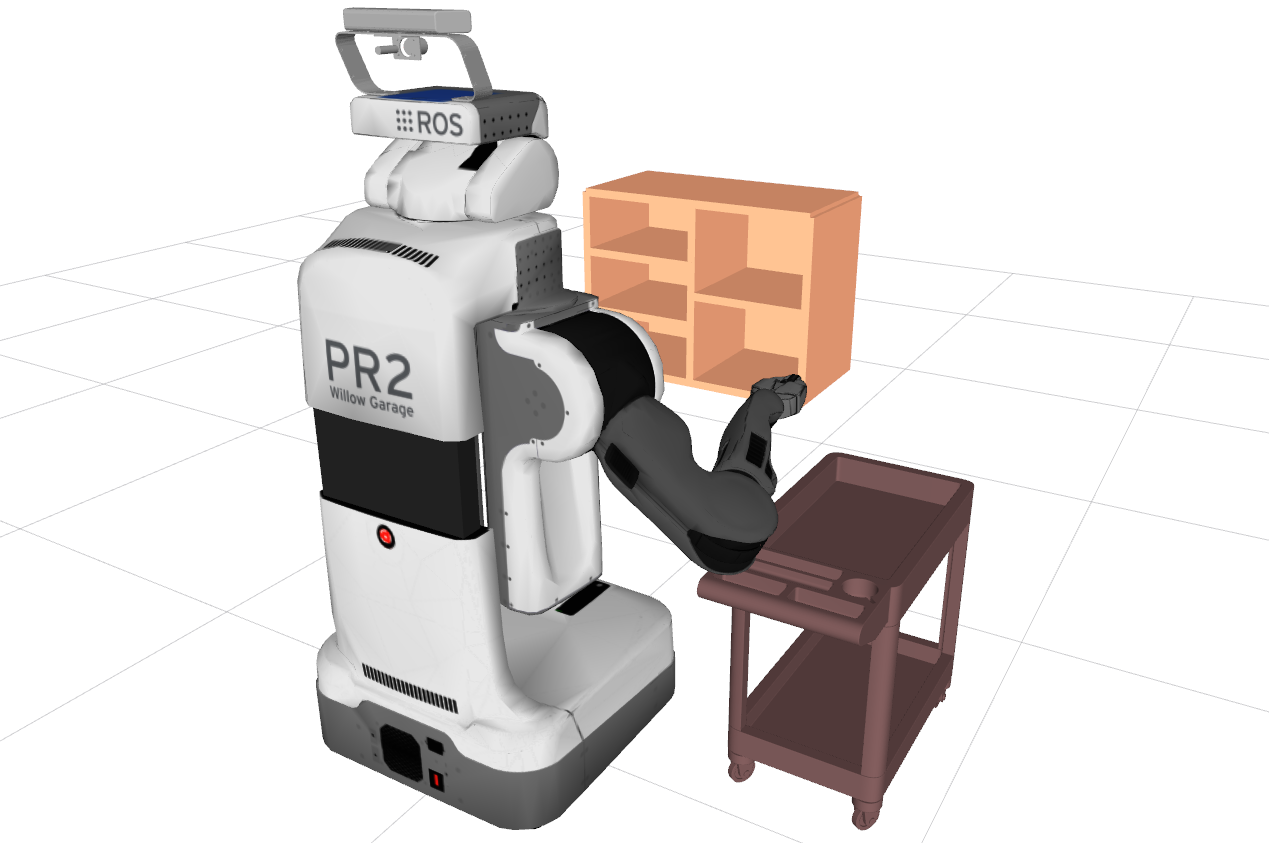
\includegraphics[width=0.8\textwidth]{pr2.png}
    % \vspace{-2mm}
  \caption{
  Motivating scenario---a robot (PR2) picking up objects from shelves and placing them into a bin.
}
    \label{fig:PR2}
% \vspace{-6mm}
\end{figure}

\section{Algorithm Framework}
\label{sec:alg}
In this section we describe our algorithmic framework. We start (Sec.~\ref{sec:pdef}) by formally defining our problem and continue (Sec.~\ref{sec:key}) by describing the key idea that enables our approach.
We then proceed (Sec.~\ref{subsec:alg}) to detail our algorithm and conclude with implementation details (Sec.~\ref{subsec:impl}).

\subsection{Problem formulation and assumptions}
\label{sec:pdef}
Let $\calC$ be the configuration space of a robot operating in a static environment containing obstacles.
We say that a configuration is valid (invalid) if the robot, placed in that configuration does not (does) collide with obstacles, respectively.
We are given in advance a start configuration~$\Sstart \in \calC$ and some goal region~$G \subset \calC$.
We emphasize that the goal region may contain invalid configurations.
In the query phase we are given multiple queries $(\Sstart, s_{\text{goal}})$ where $s_{\rm goal} \in G$ is a valid configuration (fully defined goal) and for each query, we need to compute a collision-free path connecting $\Sstart$ to $s_{\text{goal}}$.

Coming back to our motivating example of mail sorting---the start configuration would be some predefined configuration above the cart where the robot can pick up the envelopes from and the goal region would comprise of all possible placements of the robot's end effector in the cubbies. The environment is static as the only obstacles in the environment are the shelves and the cart which remain stationary in between queries.

We discretize $\calC$ into a state lattice $\calS$ such that any state~$s \in \calS$ is connected to a set of successors and predecessors via a mapping Succs/Preds: $\calS \rightarrow 2^\calS$.
Define $G_\calS := \calS \cap G$ to be the states that reside in the goal region. Note that although our approach is applicable to general graphs (directed or undirected), to be able to reuse the planned path in the reverse direction (e.g. in our motivating example for the motion from the shelve to the start configuration) the graph needs to be undirected.
We make the following assumptions:

%\begin{enumerate}[label={\textbf{A\arabic*}}]
\vspace{2mm}\begin{assumption} \label{asm:1:1} $G_\calS$ is a relatively small subset of $S$. Namely, it is feasible to exhaustively iterate over all states in $G_\calS$.
However, storing a path from $\Sstart$ to each state in $G_\calS$ is infeasible.
\end{assumption}
  
\vspace{2mm}\begin{assumption} \label{asm:1:2} The planner has access to a heuristic function $h: \calS \times \calS \rightarrow \mathbb{R}$ which can estimate the distance between any two states in $G_\calS$. Moreover, 
 \begin{itemize}
  \item The heuristic function should be \textit{weakly-monotone} with respect to $G_\calS$, meaning that $\forall s_1, s_2  \in G_\calS$ where $s_1 \neq s_2 $, it holds that,
  \begin{center}
    $h(s_1, s_2) \geq \min\limits_{s_1' \in \text{Preds}(s_1)} h(s_1', s_2)$.
  \end{center}

  \item The heuristic function $h$ should induce that the goal region is \emph{convex} with respect to $h$, meaning that $\forall s_1, s_2  \in G_\calS$ where $s_1 \neq s_2 $, it holds that,
  \begin{center}
     $\argmin\limits_{s_1' \in \text{Preds}(s_1)} h(s_1', s_2) \in G_\calS$.
  \end{center}

 \end{itemize}
 Namely, for any distinct pair of states ($s_1, s_2$) in $G_\calS$, at least one of $s_1$'s predecessors has a heuristic value less than or equal to its heuristic value.
 Moreover, the predecessor with minimal heuristic value lies in the goal region.
\end{assumption}

\vspace{2mm}\begin{assumption} \label{asm:1:3} The planner has access to a tie-breaking rule that can be used to define a total order \footnote{A total order is a binary relation on some set which is anti-symmetric, transitive, and a convex relation.} over all states with the same heuristic value.
  % to a given state.
\end{assumption}

These assumptions allow us to establish strong theoretical properties regarding the efficiency of our planner. Namely, that
within a known bounded time, we can compute a collision-free path from $\Sstart$ to any state in $G_\calS$. 


Assumption~\ref{asm:1:2} may seem too restrictive (especially convexity), imposing that the goal region cannot be of arbitrary structure. However, after we detail our algorithm (Sec.~\ref{subsec:alg}) and analyze its theoretical properties (Sec.~\ref{sec:analysis1}), we sketch how we can relax this assumption to be less restrictive.


 
\subsection{Key idea}
\label{sec:key}
Our algorithm relies heavily on the notion of a greedy search.  Thus, before we describe of our algorithm, we formally define the terms greedy predecessor and greedy search.

\vspace{2mm}
\begin{definition}
\label{def:greedy-suc}
  Let $s$ be some state and $h(\cdot)$ be some heuristic function.
  A state $s' \in \text{Preds}(s)$ is said to be a \emph{greedy} predecessor of $s$ according to $h$ if it has the minimal $h$-value among all of $s$'s predecessors.
\end{definition}
Note that 
if $h$ is weakly monotone with respect to $G_\calS$
(Assumption~\ref{asm:1:2}) 
and we have some tie-breaking rule
(Assumption~\ref{asm:1:3}), then every state has a greedy predecessor in the $G_\calS$ and it is unique.
In the rest of the text, when we use the term greedy predecessor, we assume that it is unique and in $G_\calS$.

\vspace{2mm}
\begin{definition}
  Given a heuristic function $h(\cdot)$,
  an algorithm is said to be a \emph{greedy search}  with respect to $h$ if for every state it returns its greedy predecessor according to $h$.
\end{definition}
Note that we define the greedy search in terms of the predecessors and not the successors to account for the directionality of the graph. This will become more clear in Sec.~\ref{subsec:alg}.

\textbf{Remark:} Now that we have the notion of greedy search, we can better explain our definition of convexity with respect to~$h$ (Assumption~\ref{asm:1:2});
this assumption ensures that a greedy search between any pair of states lies within the goal region, analogously to the standard notion of a convex region where for every pair of points within the region, every point on the straight line segment that joins the pair of points is also within the region.

Our key insight is to precompute in an offline phase subregions within the goal region where a greedy search to a certain (``attractor'') state is guaranteed to be collision free and use these subregions in the query phase.
Specifically, in the preprocessing phase, $G_\calS$ is decomposed into a finite  set of (possibly overlapping) subregions $\calR$.
Each subregion $R_i \in \calR$ is a hyper-ball defined using a center which we refer to as the ``attractor state''~
\sAttract and a radius $r_i$.
These subregions, which may contain invalid states, are constructed in such a way that the following two properties hold
\begin{enumerate}[label={\textbf{P\arabic*}}]
  \item \label{property:1} For any valid goal state $s_{\text{goal}} \in R_i \cap G_\calS$, a greedy search with respect to $h(s, \sAttract)$ over $\calS$ starting at $\sGoal$ will result in a collision-free path to \sAttract.
  \item \label{property:2} The union of all the subregions completely cover the valid states in $G_\calS$. 
      Namely, $\forall s \in G_\calS~\text{s.t.}~s~\text{is valid}, \exists R \in \calR \ s.t. \ s \in R$.
\end{enumerate}

In the preprocessing stage, we precompute a library of collision-free paths $\calL$ which includes a path from $\Sstart$ to each attractor state. 
In the query phase, given a query~\sGoal, we 
(i)~identify a subregion $R_i$ such that $\sGoal \in R_i$ (using the precomputed radii~$r_i$),
(ii)~run a greedy search towards~\sAttract by greedily choosing at every point the predecessor that minimizes~$h$ and
(iii)~append this path with the precomputed path in $\calL$ to $\Sstart$ to obtain the complete plan.
For a visualization of our algorithm, see Fig.~\ref{fig:approach}.


\begin{figure}
\centering
\includegraphics[width=\textwidth]{orig_version.pdf}
    % \vspace{-2mm}
  \caption{
  Visualization of approach. The discretized goal region~$G_\calS$ is shown. Subregions are depicted in green, and  obstacles are depicted in red.
  Precomputed paths from $s_{\rm{start}}$ to attractor states are depicted in blue.
 Given a query $(s_{\rm{start}}, s_{\rm{goal}})$, the returned path is given by $\pi_i$ appended with a greedy path ~$\pi_g$ from $s_{\rm{goal}}$ to \sAttract (reversed), which is depicted in purple.
}
    \label{fig:approach}
% \vspace{-6mm}
\end{figure}

\subsection{Algorithm}
\label{subsec:alg}
\subsubsection{Preprocessing Phase}
The preprocessing phase of our algorithm, detailed in Alg.~\ref{alg:1}, takes as input the start state~$\Sstart$, the goal region~$G_\calS$ and a conventional motion planner $\calP$, and outputs a set of subregions~$\calR$ and the corresponding library of paths~$\calL$ from~\Sstart to each~\sAttract. 

The algorithm covers~$G_\calS$ by iteratively finding a state $s$ not covered\footnote{Here, a state $s$ is said to be covered if there exists some subregion $R \in \calR$ such that $s \in R$.} by any subregion and computing a new subregion centered at $s$.
To ensure that $G_\calS$ is completely covered (Property~\ref{property:2}) we maintain a set~$V$ of valid (collision free) and a set $I$ of invalid (in collision) states called \emph{frontier states} (lines~\ref{alg:1:v} and~\ref{alg:1:i}, respectively).
We also construct subregions centered around invalid states~$\hat{\calR}$ to efficiently store which invalid states have been considered.
We start by initializing~$V$ with some random state in $G_\calS$ and iterate until both~$V$ and~$I$ are empty, which will ensure that $G_\calS$ is indeed covered even if $G_\calS$ is not fully connected.

At every iteration, we pop a state from $V$ (line~\ref{alg:1:pop}), and if there is no subregion covering it, we add it as a new attractor state and compute a path $\pi_i$ from $\Sstart$ (line~\ref{alg:1:path}) using the planner $\calP$.
We then compute the corresponding subregion (line~\ref{alg:1:cr} and Alg.~\ref{alg:2}).

As we will see shortly, computing a subregion corresponds to a Dijkstra-like search centered at the attractor state.
The search terminates with the subregion's radius $r_i$ and a list of frontier states that comprise of the subregion's boundary.
The valid and invalid frontier states are then added to $V$ and $I$, respectively (lines~\ref{alg:1:insert_v} and~\ref{alg:1:insert_i}).


Once $V$ gets empty the algorithm starts to search for states which are valid and yet uncovered by growing subregions around invalid states popped from~$I$ (lines~\ref{alg:1:iv_loop}-\ref{alg:1:iv_region} and detailed in Alg.~\ref{alg:3b}). If a valid and uncovered state is found, it is added to $V$ and the algorithm goes back to computing subregions centered at valid states (lines~\ref{alg:1:x_states}-\ref{alg:1:break}), otherwise if $I$ also gets empty, the algorithm terminates and it is guaranteed that each valid state contained in $G_\calS$ is covered by at least one subregion.

\begin{algorithm}[t]
%\footnotesize
\hspace*{\algorithmicindent} \textbf{Inputs:} $G_\calS$, $\Sstart$, $\calP$
\Comment{goal region, start state and a planner} 

\hspace*{\algorithmicindent} \textbf{Outputs:} 
$\calR, \calL$
%$R_i = (\sAttract, r_i)$, $\pi_i$,
\Comment{subregions and corresponding paths to $\Sstart$}

%\hspace*{\algorithmicindent}
% \textbf{Parameters:} $r_{\text{max}}$   \Comment{maximum radius of a region}
\caption{Goal Region Preprocessing}\label{alg:1}
\begin{algorithmic}[1]
\Procedure{PreprocessRegion}{$G_\calS$}
%\Procedure{PreprocessRegion}{$G, r_{\text{max}}$}
  \State $s \leftarrow$\textsc{ SampleValidState}($G_\calS$)
  \State $V \leftarrow \{ s \}$   \Comment{valid frontier states initialized to random {state}} \label{alg:1:v}
  \State $I$ = $\emptyset$   \Comment{invalid frontier states} \label{alg:1:i}
  \State $ i \leftarrow 0$
       \hspace{2mm} 
       $\calL = \emptyset$
       \hspace{2mm} 
       $\calR = \emptyset$
       \hspace{2mm} 
       $\hat{\calR} = \emptyset$
       
  \vspace{2mm}
    \While {$V$ and $I$ are not empty}
        \While {$V$ is not empty}
          \State $s \leftarrow V.\text{pop}()$ \label{alg:1:pop}
            \If {$\nexists R \in \calR$  s.t. $s \in R$ }  \label{alg:1:discard}
            \Comment{$s$ is not covered}
        \State $\sAttract \leftarrow s$               
        \label{alg:1:attract} 
                \State $\pi_i$ = $\calP.$\textsc{PlanPath}($\Sstart, \sAttract$); \label{alg:1:pp}
                \hspace{2mm }
                $\calL \leftarrow \calL \cup \{ \pi_i \}$  \label{alg:1:path}
                \State $(\text{OPEN}, r_i) \leftarrow$ \textsc{ComputeCoverage}($\sAttract$) \label{alg:1:cr}
%                \State $(\text{OPEN}, r_i) \leftarrow$ \textsc{ComputeCoverage}($\sAttract, r_{\text{max}}$) \label{alg:1:cr}
                \State insert Valid(OPEN) in $V$  \label{alg:1:insert_v}
                \State insert Invalid(OPEN) in $I$   \label{alg:1:insert_i}
                \State $R_i$ $\leftarrow$ $(\sAttract, r_i)$; 
                \hspace{2mm} $ i \leftarrow i+1$        \hspace{2mm }
                $\calR \leftarrow \calR \cup \{ R_i \}$
                            \EndIf
        \EndWhile

\vspace{2mm}        
        
        \While {$I$ is not empty} \label{alg:1:iv_loop}
            \State $s$ $\leftarrow$ $I.pop()$
      \If {$\nexists R \in \calR \cup \hat{\calR}$ s.t. $s \in R$ }      \Comment{$s$ is not covered}
\State $(X, r)$ $\leftarrow$ \textsc{FindValidUncoveredState}($s$)
%                \State $(X, r)$ $\leftarrow$ \textsc{FindValidUncoveredState}($s, r_{\text{max}}$)
                \State $\hat{R}$ $\leftarrow$ $(s,r)$;
        \hspace{2mm}
        $\hat{\calR} \leftarrow \hat{\calR} \cup \{ \hat{R} \}$ \Comment{invalid subregion}  \label{alg:1:iv_region}
                \If {$X$ is not empty}  \Comment{valid state found}  \label{alg:1:x_states}
                    \State insert $X$ in $V$
                    \State \textbf{break} \label{alg:1:break}
                \EndIf
            \EndIf
        \EndWhile
    \EndWhile

  \vspace{2mm}

  \State \Return $\calR, \calL$
\EndProcedure
\end{algorithmic}
\end{algorithm}

\begin{figure}[tb]
  \centering
    \includegraphics[width=\textwidth]{region.pdf}
    % \vspace{-2mm}
  \caption{
  Visualization of Alg~\ref{alg:2}. Subregion $R_i$ (green) grown from $\sAttract$ in a discretized goal region~$G_\calS$ with obstacles (in red). The covered states are depicted in white
  The first uncovered state is also depicted (in red). It is the state from which the greedy search will encounter an obstacle.
}
    \label{fig:alg2}
% \vspace{-6mm}
\end{figure}

\subsubsection{Coverage Search}
The core of our planner lies in the way we compute the subregions (Alg.~\ref{alg:2} and Fig.~\ref{fig:alg2}) which we call a ``Coverage Search''. The algorithm maintains a set of \emph{covered} states $S_{\text{covered}}$ for which Property~\ref{property:1} holds.
As we will see, this will ensure that in the query phase, we can run a greedy search from any covered state $s \in S_{\text{covered}}$ and it will terminate in the attractor state. 
%
The following recursive definition formally captures the notion of a covered state.

\vspace{2mm}
\begin{definition}
  Given some attractor state \sAttract, we say that a state $s \in G_\calS$ is covered under some function $h(\cdot)$ by to \sAttract if either
  (i)~$s = \sAttract$ or
  (ii)~the greedy predecessor of $s$ with respect to $h(s,\sAttract)$ is covered.
\end{definition}

The algorithm computes a subregion that covers the maximum number of states that can fit into a hyper-ball defined by $h(s,\sAttract)$. 
The search maintains a priority queue OPEN ordered according to $h(s,\sAttract)$. Initially, the successors of $\sAttract$ are inserted in the OPEN (line~\ref{alg:2:OPEN}). For each expanded successor, if its valid greedy predecessor is in $S_{\text{covered}}$, then the successor is also labeled as covered (lines~\ref{alg:2:crit} and~\ref{alg:2:set}). 

The algorithm terminates when the search pops a state which is valid but does not have a greedy predecessor state in $S_{\text{covered}}$ (line~\ref{alg:2:terminate}). Intuitively, this corresponds to  the condition when the coverage search exits an obstacle (see Fig.~\ref{fig:alg2}).
At termination, all the states within the boundary of radius $r_i$ (excluding the boundary) are covered.


\begin{algorithm}[t]
%\footnotesize
\caption{Coverage Search}\label{alg:2}

\begin{algorithmic}[1]
\Procedure{ComputeCoverage}{$\sAttract$}
%\Procedure{ComputeCoverage}{$\sAttract, r_{\text{max}}$}
\State $S_{\text{covered}} \leftarrow \{\sAttract\}$ \Comment{covered set} \label{alg:2:covered}
\State OPEN $\leftarrow \{$Succs($\sAttract$)$\}$  \Comment{key: $h(s,\sAttract)$} \label{alg:2:OPEN}
\State CLOSED $\leftarrow \emptyset$
\State $r_i \leftarrow 0$

%\While {$r_i \leq r_{\text{max}}$}
\While{OPEN$\neq \emptyset$}
    \State $s \leftarrow$ OPEN.pop()
    \State insert $s$ in CLOSED
    \State $s'_g \leftarrow \argmin\limits_{s' \in \text{Preds}(s)} h(s', \sAttract)$ 
%    \State $s'_g \leftarrow$ GreedySucc($s$)
  \label{alg:2:greedy} 
 \Comment{greedy predecessor}
 % acc. to some tie-breaking criteria}
    \If {$s'_g$ $\in$ $S_{\text{covered}}$ and Valid(edge(s,$s'_g$))}  \label{alg:2:crit}
        \State $S_{\text{covered}} \leftarrow S_{\text{covered}} \cup \{s\}$  \Comment{$s$ is greedy} \label{alg:2:set}
    \ElsIf {Valid($s$)} \label{alg:2:terminate}
        \State $r_i \leftarrow h(s, \sAttract)$ \label{alg:2:rad}
        \State \Return (OPEN, $r_i$)
%        \State break
    \EndIf
    \For {each $s' \in \text{Succs}(s) \cap G_\calS$} \label{alg:2:prun}
        \If {$s' \notin$ CLOSED}
            \State insert $s'$ in OPEN with priority $h(s', \sAttract)$
        \EndIf
    \EndFor
\EndWhile
\State $r_i \leftarrow h(s, \sAttract) + \epsilon$    \Comment{$\epsilon$ is a small positive constant}
\State \Return (OPEN, $r_i$)

\EndProcedure
\end{algorithmic}
\end{algorithm}

\begin{algorithm}[t]
%\footnotesize
\caption{Find valid uncovered state}\label{alg:3b}

\begin{algorithmic}[1]
\Procedure{FindValidUncoveredState}{$\hat{s}$}
\State OPEN $\leftarrow \{\hat{s}\}$
\While{OPEN$\neq \emptyset$}
  \State $s \leftarrow$ OPEN.pop()
  \State insert $s$ in CLOSED
  \If {$\nexists R \in \calR$  s.t. $s \in R$ and Valid(s)}
  % \Comment{$s$ is not covered and $s$ is valid}
    \State \Return ($\{s\}$, $h$($s$, $\hat{s}$))
  \EndIf
  \For {each $s' \in \{\text{Succs}(s) \cup \text{Preds}(s)\} \cap G_\calS$}
    \If {$s' \notin$ CLOSED}
        \State insert $s'$ in OPEN with priority $h(s', \sAttract)$
    \EndIf
  \EndFor
\EndWhile
\State $r = h$($s$, $\hat{s})) + \epsilon$    \Comment{$\epsilon$ is a small positive constant}
\State \Return ($\emptyset$, $r$))
\EndProcedure
\end{algorithmic}
\end{algorithm}


\subsubsection{Query Phase}
Given a query goal state $s_{\text{goal}} \in G_\calS$ 
our algorithm, detailed in Alg.~\ref{alg:3}, starts by finding a subregion $R_i \in \calR$ which covers it (line.~\ref{alg:3:covers}). Namely, a subregion~$R_i$ for which 
$h(s_{\text{goal}}, \sAttract) < r_i$.
We then run a greedy search starting from $s_{\text{goal}}$ by iteratively finding for each state $s$ the predecessor with the minimum heuristic $h(s, \sAttract)$ value until the search reaches \sAttract (lines~\ref{alg:3:greedy-call} and~\ref{alg:3:greedy-call-start}-~\ref{alg:3:greedy-call-end}). 
The greedy path~$\pi_g$ is then appended to the corresponding precomputed path~$\pi_i \in \calL$ (line~\ref{alg:3:return}). 
Note that at no point  do we need to perform collision checking in the query phase (given the fact that the environment is static).

\begin{algorithm}[t]
\hspace*{\algorithmicindent} \textbf{Inputs:} $G_\calS, \calL, \calR$

\hspace*{\algorithmicindent} \textbf{Output:} $\pi$	\Comment{full path from \sStart to \sGoal}
%\footnotesize
\caption{Query}\label{alg:3}

\begin{algorithmic}[1]
\Procedure{FindGreedyPath}{$s_1, s_2$}
  \label{alg:3:greedy-call-start}
  \State $s_{\text{curr}} \leftarrow s_2$; \hspace{2mm} $\pi \leftarrow \emptyset$
  \While{$s_{\text{curr}} \neq s_1$} \label{alg:3:while}
    \State $\pi \leftarrow \pi \cdot s_{\text{curr}}$
    \Comment{append current state to path}
      \State $s_{\text{curr}} \leftarrow \argmin\limits_{s \in \text{Preds}(s_{\text{curr}})} h(s, s_1)$  \Comment{greedy predecessor}
    \EndWhile
    \State \Return \textsc{Reverse} ($\pi$)   \Comment{reverse to get a path from $s_1$ to $s_2$}
\EndProcedure
\label{alg:3:greedy-call-end}

\vspace{2mm}

\Procedure{ComputePath}{$\sGoal$}
  \For {each $R_i \in \calR$}
    \If {$h(s_{\text{goal}}, \sAttract) < r_i$}
    \Comment{$R_i$ covers $\sGoal$}
    \label{alg:3:covers}
      \State $\pi_g \leftarrow$ \textsc{FindGreedyPath} ($\sAttract, \sGoal$)
      \label{alg:3:greedy-call}
      \State \Return $\pi_i \cdot \pi_g$  \Comment{append $\pi_g$ to~$\pi_i \in \calL$}
      \label{alg:3:return}
    \EndIf
  \EndFor

\EndProcedure
\end{algorithmic}
\end{algorithm}


\section{Analysis}
\label{sec:analysis1}
In this section we formally prove that 
our algorithm is correct (Sec.~\ref{subsec:correct}) and 
analyze its computational complexity and bound on solution quality (Sec.~\ref{subsec:complexity} and ~\ref{subsec:quality} respectively).

\subsection{Correctness}
\label{subsec:correct}
To prove that our algorithm is correct, we show that indeed all states of every subregion are covered and we can identify if a state belongs to a subregion using its associated radius.
Furthermore, we show that a path obtained by a greedy search within any subregion is valid and that all states in $G_\calS$ are covered by some subregion.
These notions are captured by the following set of lemmas.

\vspace{2mm}
\begin{lemma}
\label{lemma:covered-1}
Let $S_{\text{covered}}$ be the set of states computed by Alg.~\ref{alg:2} for some attractor vertex \sAttract.
%
Every state $s \in S_{\text{covered}}$ is covered by \sAttract.
\end{lemma}
%
\begin{proof}
The proof is constructed by an induction over the states added to $S_{\text{covered}}$.
The base of the induction is trivial as the first state added to $S_{\text{covered}}$  is \sAttract (line~\ref{alg:2:covered}) which, by definition, is covered by \sAttract.
%
A state $s$ is added to $S_{\text{covered}}$ only if its greedy predecessor is in $S_{\text{covered}}$ (line~\ref{alg:2:greedy}) which by the induction hypothesis is covered by \sAttract.
This implies by definition that $s$ is covered by \sAttract.
%
Note that this argument is true because the greedy predecessor of every state is unique (Assumption~\ref{asm:1:3}).
\end{proof}

\begin{lemma}
\label{lemma:covered-2}
Let $S_{\text{covered}}$ be the set of states computed by Alg.~\ref{alg:2} for some attractor vertex \sAttract.
%
A state $s$ is in $S_{\text{covered}}$ iff $h(s, \sAttract) < r_i$.
\end{lemma}

\begin{proof}
Alg.~\ref{alg:2} orders the nodes to be inserted to $S_{\text{covered}}$ according to $h(s, \sAttract)$ (line~\ref{alg:2:OPEN}).
As our heuristic function is weakly monotonic (Assumption~\ref{asm:1:2}), the value of $r_i$ monotonically increases as the algorithm adds states to $S_{\text{covered}}$ (line~\ref{alg:2:rad}).
Thus, for every state $s \in S_{\text{covered}}$, we have that $h(s, \sAttract) < r_i$.

For the opposite direction, assume that there exists a state $s \notin S_{\text{covered}}$ such that $h(s, \sAttract) < r_i$.
This may be because  Alg.~\ref{alg:2} terminated due to a node $s'$ that was popped from the open list with 
$h(s', \sAttract) \leq h(s, \sAttract)$.
However, using the fact that our heuristic function is weakly monotonic (Assumption~\ref{asm:1:2}) we get a contradiction to the fact that $h(s, \sAttract) < r_i$.
Alternatively, this may be because we prune away states that are in $G_\calS$  (Alg.~\ref{alg:2} line~\ref{alg:2:prun}).
However, using the fact that our goal region is convex with respect to $h$ (Assumption~~\ref{asm:1:2}), this cannot hold.
\end{proof}

\begin{lemma}
\label{lemma:greedy}
Let $R_i \in \calR$ be a subregion computed by Alg.~\ref{alg:2}.
for some attractor vertex \sAttract.
% 
A greedy search with respect to $h(s, \sAttract)$  starting from any valid state $s \in R_i$ is complete and valid.
\end{lemma}

\begin{proof}
Given a state $s \in R_i$, we know that $s \in S_{\text{covered}}$ (Lemma~\ref{lemma:covered-2})
and that it is covered by \sAttract (Lemma~\ref{lemma:covered-1}).
%
It is easy to show (by induction) that any greedy search starting at a state $S_{\text{covered}}$ will only output states in $S_{\text{covered}}$.
Furthermore, a state is added to $S_{\text{covered}}$ only if the edge connecting to its greedy predecessor is valid (line~\ref{alg:2:crit}).
Thus, if $s\in S_{\text{covered}}$ is valid, the greedy search with respect to $h(s, \sAttract)$  starting from $s$ is complete and valid.
\end{proof}

\begin{lemma}
\label{lemma:coverage}
At the end of Alg.~\ref{alg:1}, every state $s \in G_\calS$ is covered by at least one subregion $R \in \calR$.
\end{lemma}
\begin{proof}
Assume that this does not hold and let $s \in G_\calS$ be a state that is not covered by any subregion but has a neighbor (valid or invalid) that is covered.
%
If $s$ is valid, then it would have been in the valid frontier states $V$ and either been picked to be an attractor state (line~\ref{alg:1:attract}) or covered by an existing subregion (Alg.~\ref{alg:2}).
%
A similar argument holds if $s$ is not valid.
\end{proof}

From the above we can immediately deduce the following corollary:

\vspace{2mm}

\begin{cor}
  After preprocessing the goal region~$G_\calS$ (Alg.~\ref{alg:1} and~\ref{alg:2}), in the query phase we can compute a valid path for any valid state $s \in G_\calS$ using Alg.~\ref{alg:3}.
\end{cor}


\textbf{Remark}
We can relax Assumption~\ref{asm:1:2} in two ways.
The first is by explicitly tracking states not in the goal region instead of pruning them away (Alg.~\ref{alg:2} line~\ref{alg:2:prun}).
Unfortunately, this may require the algorithm to store many states not in $G_\calS$  which may be impractical (recall that Assumption~\ref{asm:1:1} only states that we can exhaustively store in memory the states in the goal region).
An alternative, more practical way, to relax Assumption~\ref{asm:1:2}  is by terminating the search when we  encounter a state not in the goal region.
This may cause the algorithm to generate much more subregions (with smaller radii) which may increase the memory footprint and the preprocessing times.


\subsection{Complexity}
In this section we will do an asymptotic analysis of the time and memory complexities of our algorithm for the worst-case.

The complexity analysis makes the following global assumptions.
\vspace{2mm}\begin{assumption}
\label{asm:1:4} $|\calR| \ll n_{G_{\calS}}$ where~$n_{G_{\calS}}$ is the total number of goals in~$G_\calS$
\end{assumption}
\vspace{2mm}\begin{assumption}
\label{asm:1:5} $G_\calS$ is fragmented such that $|\calR|$ is upper-bounded by a constant
\end{assumption}
%\vspace{2mm}\begin{assumption}
%\label{assum:8} The time it takes to expand a state~(single iteration of loop at Alg.~\ref{alg:3}, line~\ref{alg:3:while}) is less than the time it takes for a robot to execute one action.
%\end{assumption}

\label{subsec:complexity}
\subsubsection{Time Complexity}
We define the variable~$\calD$ as depth (maximal number of expansions of a greedy search) of the largest subregion. We can measure the depth of each subregion in Alg.~\ref{alg:2} by keeping track of the depth of each expanded state from the root i.e., $\sAttract$.
%
\vspace{2mm}
\begin{lemma}
\label{lemma:unboundedD}
Given the number of subregions~$|\calR|$ and the depth of the largest subregion~$\calD$, full path can be found in~$O(\calD)$ time
\end{lemma}

\begin{proof}
The query time comprises of 
(i)~finding the containing subregion $R_i$
(ii)~running the greedy search to $\sAttract$.
Step~(i) requires iterating over all subregions (in the worst case) which takes $O(|\calR|)$ steps while 
step~(ii) requires expanding the states along the path from $\sGoal$ to $\sAttract$ which requires~$O(\calD)$ expansions.
For each expansion we need to find the greedy predecessor, considering at most $b$ predecessors, where $b$ is the maximal branching factor of our graph.
Hence, overall the query phase takes $O(|\calR| + \calD \cdot b)$ operations. Since~$|\calR|$ is upper bounded by a constant~(from assumption~\ref{asm:1:5}) and~$b$ is a constant factor, the time complexity thus becomes~$O(\calD)$.
\end{proof}

Note that we can also bound the number of expansions required for the query phase by bounding the maximum depth of the subregions~$\calD$. We can do that by terminating Alg.~\ref{alg:2} when the $R_i$ reaches the depth bound or if the existing termination condition (line~\ref{alg:2:terminate}) is satisfied. Having said that, this will come at the price of increasing the number of subregions and the assumption~\ref{asm:1:5} will also not hold anymore. To give an intuition, we can draw an analogy with the sphere packing problem~\cite{hales1992sphere}; for a required volume to be covered, if the radii of the spheres is fixed, then the number of spheres needed to cover the volume will not be bounded by a constant but will be a function of the size of the volume.

\vspace{2mm}
\begin{lemma}
\label{lemma:OrderR}
	Given the number of subregions~$|\calR|$ and bounded~$\calD$, full path can be found in~$O(|\calR|)$ time
\end{lemma}

Now we consider a special case for which the algorithm has~$O(1)$ complexity.

\vspace{2mm}
\begin{lemma}
\label{lemma:o1}
	For the case when ~$|\pi_g| \leq c*|\pi_i|$, where~$c \geq 1$ is a constant integer, each action requires~$O(1)$ time delibration
\end{lemma}

\begin{proof}
	Here $|\cdot|$ denotes the length of the paths. This lemma can be trivally proved from assumptions~\ref{asm:1:5} and by interleaving planning and execution. From assumption~\ref{asm:1:5}, the time required to find the containing subregion~$R_i$ is bounded by a constant. Once~$R_i$ is found, the robot can find the greedy path~$\pi_g$ while it executes~$\pi_i$ by interleaving planning and execution.
	Since~$|\pi_g|$ is bounded by ~$c*|\pi_i|$, expanding~$c$ states~($O(1)$ operation) for each step traversal along~$|\pi_i|$, the greedy search will find~$\pi_g$ by the time robot arrives at~$\sAttract$.	
%	
%If~$|\pi_i| > |\pi_g|$ and the assumption~\ref{assum:8} holds, by the time the robot reaches the~$\sAttract$,~$\pi_g$ will be computed and can be executed by the robot.
\end{proof}

%
%\textbf{Constant-time Complexity}
%We need to show that $O(|\calR| + \calD \cdot b) \rightarrow O(1)$. While~$\calD$ and~$b$ are constants,~$|\calR|$ is not a constant and does not have a bound and so the complexity of the query phase as is is~$O(|\calR|$ which is linear in~$|\calR|$.
%Here we propose a modification or extension of the full algorithm (both preprocessing and query phases) which is detailed in section~\ref{sec:extension} which will make the complexity constant time. The extension allows us to specify a constant upper bound on~$|\calR|$.  
%Now recall the definition of the constant-time algorithm from section~\ref{sec:ctmp}. Irrespective of the size of input to the algorithm, since ~$|\calR|$ has a constant upper bound and $\calD$ and~$b$ are constants, the query phase has constant-time complexity i.e.~$O(1)$.
%
%Note that in~$O(|\calR| + \calD \cdot b)$,~$\calD$ and~$b$ are trivially bounded; both are constants. The third term~$|\calR|$ however depends on goal region~$G_\calS$. Roughly speaking,~$|\calR|$ depends on three things~(1) how cluttered~$G_\calS$ is with obstacles, the more cluttered it is the more subregions we will get~(2) the size of~$G_\calS$; a bigger goal region will render more subregions and~(3) the parameter~$\calD$. We make the assumption that for a choice of~$\calD$~(large enough), for certain degree of obstacle clutter in C-space~(less enough) and by our original problem formulation that the goal region is a small subset of the C-space, the upper bound on~$|\calR|$ is bounded independently of the size of~$G_\calS$. Under this analysis we can conclude that the algorithm has a constant time complexity i.e~$O(1)$.
%
\subsubsection{Space Complexity}
This section analyses the worst-case space complexity of the metadata generated after the preprocessing phase that is then used in the query phase.
\vspace{2mm}
\begin{lemma}
	Given the number of subregions~$|\calR|$ and unbounded~$\calD$, the algorithm requires~$O(|\pi_{\text{max}}|)$ space.
\end{lemma}
\begin{proof}
	The preprocessing phase generates metadata of size~$O(|\pi_{\text{max}}| \cdot |\calR|)$ where $|\pi_{\text{max}}|$ is the length of the longest precomputed path in~$\calL$. Since~$\calR$ is upper bounded by a constant~(assumption~\ref{asm:1:5}) and also because~$|\calR| \ll n$~(assumption~\ref{asm:1:4}) the algorithm requires~$O(|\pi_{\text{max}}|)$ space.
\end{proof}

\vspace{2mm}
\begin{lemma}
	Given the number of subregions~$|\calR|$ and bounded~$\calD$, the algorithm requires~$O(|\pi_{\text{max}}| \cdot |\calR|)$ space.
\end{lemma}
\begin{proof}
	Enforcing a bound on~$\calD$ breaks assumption~\ref{asm:1:5} as explained earlier in the analysis. This introduces~$|\calR|$ as a factor in the space complexity.
\end{proof}

%$\Tbound$ and ~$T_\textrm{const}$
\subsection{CTMP-Completeness}
We now analyse the algorithm under the CTMP-Completeness criteria described in chapter~\ref{sec:ctmp} for the special case of Lemma~\ref{lemma:o1}. Since the algorithm requires~$O(1)$ time to plan the next action, $T_\textrm{const}$ is constant-time bounded and can be deduced from the empirical analysis of the algorithm.
%
The constant~$c$ can be deduced from the specified time budget~$\Tbound (> T_\textrm{const})$. The larger the~$\Tbound$, the larger the number of actions $c$, that the algorithm can plan per action execution.
%
Furthermore, Lemma~\ref{lemma:greedy} assures that the greedy path~$\pi_g$ does not contain cycles, otherwise the greedy search would be incomplete. Hence from lemmas~\ref{lemma:o1} and~\ref{lemma:greedy} and by Definition.~\ref{def:complete} we have the following theorem.

\vspace{2mm}
\begin{theorem}
	The algorithm is CTMP-Complete.
%	By Def.~\ref{ctmp:def} and from lemmas~\ref{lemma:o1} and~\ref{lemma:greedy}, the algorithm is a CTMP algorithm.
\end{theorem}

We also have the following corollary.

\vspace{2mm}
\begin{cor}
	The algorithm can be used for non-stop execution under the condition~$\Tconst < \Texec$
\end{cor}

%\subsection{Algorithm Completeness}
%\label{subsec:completeness}
%Our method generates plans by stitching together a path from the library $\calL$ (computed offline using some planner~$\calP$), and a path computed online which is returned by the greedy search on a discretized graph $G_\calS$. For the former, our method simply inherits the completeness properties of the planner $\calP$, whereas for the latter, our method is resolution complete; it follows from the correctness discussion (Section~\ref{subsec:correct}).

\subsection{Bound on Solution Quality}
\label{subsec:quality}
Let the function $c(\cdot)$ denote the cost of a path and $c^*(\cdot)$ denote the cost of an optimal path. Assuming that we precompute each path $\pi_i \in \calL$ with the optimal cost $c^*(\pi_i)$, from the triangle inequality it can be trivially shown that the quality of complete path $\pi$ computed by our method has an additive suboptimality bound; i.e.,
 % \begin{center}
 $c(\pi) - c^*(\pi) < 2 * c(\pi_g)$,
 % \end{center}
where $c(\pi_g)$ is the cost of the greedy path from the attractor to the goal state.

%\ignore{
%\section{Algorithm Extension}
%\label{sec:extension}
%In section~\ref{sec:analysis}, we enforced a bound on the number of subregions to guarantee~$O(1)$ complexity. If we do so Alg.~\ref{alg:1} may terminate without covering the~$G$ fully.
%The key idea of the following algorithm extension is to change the method of finding the attractor given a goal from geometric checks~(using radii of subregions) to a hash lookup which is a constant time operation. For doing so, the algorithm needs to pay an extra price in terms of memory, since now it has to store the goals in~$G_\calS$ and associated attractors in a lookup table. The new method differs both in preprocessing and query phases and is explained in this section.
%
%\subsection{Preprocessing Phase and Coverage Search}
%In case the upper bound on the number of subregions is reached in Alg.~\ref{alg:1} before termination, the algorithm switches to Alg.~\ref{alg:grp2}. The key difference is that instead of computing new geometric subregions~$R_i$, the algorithm maintains a lookup table~$\calM$ mapping the goals to their corresponding attractors computed during the coverage search. The modified coverage search is algorithm is detailed in Alg.~\ref{alg:cover2}. The two main differences in the coverage search are that OPEN need not be a priority queue; it can be an unordered queue and the termination condition that was there in Alg.~\ref{alg:2} is removed.
%
%\subsection{Query phase}
%
%
%%% Main Alg
%
%\begin{algorithm}[t]
%%\footnotesize
%\hspace*{\algorithmicindent} \textbf{Inputs:} $G_\calS$, $\Sstart$, $\calP$
%\Comment{goal region, start state and a planner} 
%
%\hspace*{\algorithmicindent} \textbf{Outputs:} 
%$\calL$,
%$\calM$
%%$R_i = (\sAttract, r_i)$, $\pi_i$,
%\Comment{Library of paths to $\Sstart$ and a lookup table}
%\caption{Goal Region Preprocessing}\label{alg:grp2}
%\begin{algorithmic}[1]
%\Procedure{PreprocessRegion}{$G_\calS$}
%  \State $V \leftarrow$\textsc{ GetAllValidStates}($G_\calS$)
%  \State $ i \leftarrow 0$
%       \hspace{2mm} 
%       $\calL = \emptyset$
%       \hspace{2mm} 
%       $\calM = \emptyset$
%       
%  \vspace{2mm}
%    %\While {$V$ and $I$ are not empty}
%        \While {$V$ is not empty}
%          \State $s \leftarrow V.\text{pop}()$ %\label{alg:1:pop}
%            %\If {$s$ is not covered}  %\label{alg:1:discard}
%           % \Comment{$s$ is not covered}
%        \State $\sAttract \leftarrow s$               
%        %\label{alg:1:attract} 
%                \State $\pi_i$ = $\calP.$\textsc{PlanPath}($\Sstart, \sAttract$); %\label{alg:1:pp}
%                \hspace{2mm }
%                $\calL \leftarrow \calL \cup \{ \pi_i \}$  %\label{alg:1:path}
%                \State $S_{\text{covered}} \leftarrow$ \textsc{ComputeCoverage}($\sAttract$) %\label{alg:1:cr}
%                \State insert lookup enteries $S_{\text{covered}} \rightarrow \sAttract$ in~$\calM$
%                \State $V \leftarrow V \backslash S_{\text{covered}}$;
%                \hspace{2mm} $ i \leftarrow i+1$
%
%        \EndWhile
%
%  \vspace{2mm}
%
%  \State \Return $\calL, \calM$
%\EndProcedure
%\end{algorithmic}
%\end{algorithm}
%
%%%%%%%%%%%%%%%%%%%%%%%%%%%%%%%%%%%%%%%%%%%%%%%%%%%%%%%
%\begin{algorithm}[t]
%%\footnotesize
%\caption{Coverage Search}\label{alg:cover2}
%
%\begin{algorithmic}[1]
%\Procedure{ComputeCoverage}{$\sAttract$}
%%\Procedure{ComputeCoverage}{$\sAttract, r_{\text{max}}$}
%\State $S_{\text{covered}} \leftarrow \{\sAttract\}$ \Comment{covered set} %\label{alg:2:covered}
%\State OPEN $\leftarrow \{$Succs($\sAttract$)$\}$  %\Comment{key: $h(s,\sAttract)$}% \label{alg:2:OPEN}
%\State CLOSED $\leftarrow \emptyset$
%\State $r_i \leftarrow 0$
%
%%\While {$r_i \leq r_{\text{max}}$}
%\While{OPEN$\neq \emptyset$}
%    \State $s \leftarrow$ OPEN.pop()
%    \State insert $s$ in CLOSED
%    \State $s'_g \leftarrow \argmin\limits_{s' \in \text{Preds}(s)} h(s', \sAttract)$ 
%%    \State $s'_g \leftarrow$ GreedySucc($s$)
%  %\label{alg:2:greedy} 
% \Comment{greedy predecessor}
% % acc. to some tie-breaking criteria}
%    \If {$s'_g$ $\in$ $S_{\text{covered}}$ and Valid(edge(s,$s'_g$))} % \label{alg:2:crit}
%        \State $S_{\text{covered}} \leftarrow S_{\text{covered}} \cup \{s\}$  \Comment{$s$ is greedy}% \label{alg:2:set}
%    \EndIf
%    \For {each $s' \in \text{Succs}(s) \cap G_\calS$}% \label{alg:2:prun}
%        \If {$s' \notin$ CLOSED}
%            \State insert $s'$ in OPEN with priority $h(s', \sAttract)$
%        \EndIf
%    \EndFor
%\EndWhile
%%\State $r_i \leftarrow h(s, \sAttract) + \epsilon$    \Comment{$\epsilon$ is a small positive constant}
%\State \Return $S_{\text{covered}}$
%
%\EndProcedure
%\end{algorithmic}
%\end{algorithm}
%
%%%%%%%%%%%%%%%%%%%%%%%%%%%%%%%%%%%%%%%%%%%%%%%%%%
%\begin{algorithm}[t]
%\hspace*{\algorithmicindent} \textbf{Inputs:} $G_\calS$, $\calM$, $\calL$
%
%\hspace*{\algorithmicindent} \textbf{Output:} $\pi$	\Comment{full path from \sStart to \sGoal}
%%\footnotesize
%\caption{Query}\label{alg:3}
%
%\begin{algorithmic}[1]
%
%%\Procedure{FindGreedyPath}{$s_1, s_2$}
%%  \label{alg:3:greedy-call-start}
%%  \State $s_{\text{curr}} \leftarrow s_2$; \hspace{2mm} $\pi \leftarrow \emptyset$
%%  \While{$s_{\text{curr}} \neq s_1$}
%%    \State $\pi \leftarrow \pi \cdot s_{\text{curr}}$
%%    \Comment{append current state to path}
%%      \State $s_{\text{curr}} \leftarrow \argmin\limits_{s \in \text{Preds}(s_{\text{curr}})} h(s, s_1)$  \Comment{greedy predecessor}
%%    \EndWhile
%%    \State \Return \textsc{Reverse} ($\pi$)   \Comment{reverse to get a path from $s_1$ to $s_2$}
%%\EndProcedure
%%\label{alg:3:greedy-call-end}
%%
%%\vspace{2mm}
%
%\Procedure{ComputePath}{$\sGoal$}
% % \For {each $R_i \in \calR$}
%    %\If {$h(s_{\text{goal}}, \sAttract) < r_i$}
%    %\Comment{$R_i$ covers $\sGoal$}
%    \State $\sAttract \leftarrow \calM$.\textsc{LookupAttractor}($\sGoal$)
%    %\label{alg:3:covers}
%      \State $\pi_g \leftarrow$ \textsc{FindGreedyPath} ($\sAttract, \sGoal$)
%     % \label{alg:3:greedy-call}
%      \State \Return $\pi_i \cdot \pi_g$  \Comment{append $\pi_g$ to~$\pi_i \in \calL$}
%     % \label{alg:3:return}
%    %\EndIf
%  %\EndFor
%
%\EndProcedure
%\end{algorithmic}
%\end{algorithm}
%}

\section{Implementation details}
\label{subsec:impl}

\subsection{Ordering subregions for faster queries}
Recall that in the query phase we iterate over all subregions to find one that covers \sGoal. 
In the worst case we will have to go over all subregions.
However,  our algorithm typically covers most of the goal region $G_\calS$ using a few very large subregions (namely, with a large radii~$r_i$) and the rest of $G_\calS$ is covered by a number of very small subregions.

Thus, if we order our subregions (offline) according to their corresponding radii, there is a higher chance of finding a covering subregion faster. While this optimization does not change our worst-case analysis (Sec.~\ref{sec:analysis1}), it speeds up the query time in case the number of subregions is very large.

\subsection{Using Hash Table for Singletons}
In experiments we notice that the distribution of the subregions as a function of the radii is skewed towards smaller regions and a significant number of regions are merely singletons i.e. regions having a single state. In order to decrease the query time we can store all these states in a hash table mapping each singleton to the precomputed path~$\pi_i \in \calL$.  In the query phase, this lookup table can be queried before doing the linear search through all the subregions or the vice versa depending on which operation is faster experimentally. The lookup can be performed in constant time~(worst-case)~\cite{czech1997perfect}. Complementing the preprocessed data with a lookup table improves the average query times.

\subsection{Using Efficient Nearest Neighbor Datastructures}
Using an efficient nearest neighbor data structure to store the subregions like kdtrees~\cite{bentley1975multidimensional} or cover trees~\cite{beygelzimer2006cover} etc. can reduce the time complexity of the query phase. The radii of the subregions can be included as an extra dimension to the states and specialised metric for the nearest neighbor data structure can be used to find the subregion containing the state.


\subsection{Efficiently constructing $\calL$}
Constructing paths to the attractor states (Alg.~\ref{alg:1}, line~\ref{alg:1:pp}) can be done using any motion planning algorithm $\calP$.
In our implementation we chose to use RRT-Connect~\cite{KL00}.
Interestingly, this step dominates the running time of the preprocessing step.
%
To improve the preprocessing time, we initially set a small timeout for RRT-Connect to compute a path from an attractor state $\Sstart$ to $\sAttract$.
Attractor states for which RRT-Connect fails to find a path to $\sAttract$ are marked as \textit{bad} attractors and we do not grow the subregions from them. 
These, so-called \textit{bad} attractors are discarded when other subregions cover them.

When Alg.~\ref{alg:1} terminates, we reload the valid list $V$ with the remaining bad attractors and rerun Alg.~\ref{alg:1} but this time with a large timeout for RRT-Connect. 
%
We can also increase the timeout with smaller increments and run Alg.~\ref{alg:1} iteratively until there are no more bad attractors (assuming that there exists a solution for each goal state $\in$ $G_\calS$).


\subsection{Pruning redundant subregions}
To reduce the number of precomputed subregions we remove redundant ones after the Alg.~\ref{alg:1} terminates. 
In order to do that, we iterate through all the subregions and remove the ones which are fully contained within any other subregion. 
%Note that this is possible the way Alg.~\ref{alg:1} is designed. 
This step reduces both the query complexity (see Sec.~\ref{sec:analysis1}) as well as the memory consumption.

\subsection{Interleaving Planning and Execution}
\label{subsubsec:interleave}
We know that in the query phase we have access to the precomputed library of paths~$\calL$, that stores paths from~$\sStart$ to all the attractors. Instead of computing the full path from~$\sStart$ from~$\sGoal$ and then executing it, the robot can start executing the path~$\pi_i$ (path from~$\sStart$ to~$\sAttract$) and run Alg.~\ref{alg:1:attract} in parallel. If the execution time of path~$\pi_i$ is greater than that of running Alg.~\ref{alg:1:attract}, the planning time will reduce to merely the time it takes to identify the subregion~$\R_i$.


\section{Experimental Results}
\label{sec:eval1}

\subsection{Mail Sorting Task}

We evaluated our algorithm on the PR2 robot for a single-arm (7-DOF) motion-planning problem. The illustrated task here is to pick up envelopes from a cart and put them in the cubby shelves (see Fig.~\ref{fig:PR2}). Such settings are common in mailroom environments where the robot may have to encounter the same scenario over and over again. The start state is a fixed state corresponding to the pickup location, whereas the task-relevant goal region~$G$ is specified by bounding the position and orientation of the end effector. For this domain, we define~$G$ as a bounding box covering all possible positions and orientations of the end effector within the cubby shelf.

The search is done on an implicit graph $G_\calS$ constructed using $\textit{motion primitives}$ which are small kinematically feasible motions. We define the primitives in the task-space respresentation as small motions for the robot end effector in position axes ($\textit{x, y, z}$) and orientation axes of Euler angles ($\textit{roll, pitch, yaw}$), and a joint-angle motion for the redundant joint of the 7-DOF arm. 
The heurstic function is the Euclidean distance in these seven dimensions. The discretization we use for the graph $G_\calS$ is 2~cm for the position axes, 10 degrees for the Euler axes and 5 degrees for the redundant joint. 
For this domain, we keep the $\textit{pitch}$ and $\textit{roll}$ of the end effector fixed and allow motion primitives along the remaining five dimensions i.e. $\textit{x, y, z, yaw}$ and the reduntant joint angle. We also limit the $\textit{yaw}$ to be between -30 and 30 degrees. Note that the specification of the $G_\calS$ is purely task specific and we exploit the task constraints to limit the size of $G_\calS$ which makes our preprocessing step tractable (Assumption~\ref{asm:1:1}).

We compared our approach with different single- and multi-query planners in terms of planning times, success rates and memory consumption (see Table~\ref{tab:stats}) for 200 uniformly sampled goal states from $G$. Among the multi-query planners, we implemented PRM, a multi-query version of RRT which we name MQ-RRT and the E-graph planner. 
For MQ-RRT, we precompute an RRT tree rooted at  $\Sstart$ offline (similar to PRM) and query it by trying to connect $\sGoal$ to the nearest nodes of the precomputed tree. We use the same connection strategy for MQ-RRT as the one that the asymptotically-optimal version of PRM uses\footnote{In order for the quality of paths obtained the PRM to converge to the quality of the optimal solution, a query should be connected to its $k$ nearest neighbors where 
$k = e(1+1/d)\log(n)$.
Here $n$ is the number of nodes in the tree/roadmap and $d$ is the dimensionality of the configuration space~\cite{karaman2011sampling,SSH16}. 
}.
For PRM, we precomputed the paths from all the nodes in~$G$ to~$s_{\text{start}}$ (this is analogous to our library~$\calL$). 
The query stage thus only required the connect operation (i.e. attempting to connect to $k$ nearest neighbors of $\sGoal$). For both of these planners we also added a goal-region bias by directly sampling from~$G$, five percent of the time\footnote{We used OMPL~\cite{SMK12} for comparisons with the sampling-based planners and modified the implementations as per needed.}. 

For single-query planning, we only report the results for RRT-Connect as it has the fastest run times from our experience. For PRM and MQ-RRT, if the connect operation fails for a query, we considered that case as a failure. For RRT-Connect, we set a timeout of 10 seconds.

For our method, preprocessing (Alg.~\ref{alg:1}) took 1,445 seconds and returned 1,390 subregions. For precomputing paths (Alg.~\ref{alg:1}, line~\ref{alg:1:pp}), we use RRT-Connect. For the first run of Alg.~\ref{alg:1}, we set the timeout to be 10 seconds and for the second run (after reloading $V$ with the bad attractors), we set the timeout to be 60 seconds. By doing so the algorithm finishes successfully with having no remaining bad attractors.

Table~\ref{tab:stats} shows the numerical results of our experiments. Our method being provably guaranteed to find a plan in bounded time, shows a success rate of 100 percent. For the two preprocessing-based planners PRM and MQ-RRT, we report the results for a preprocessing time of 4T (T being the time consumed by our method in preprocessing). The E-graph planner is bootstrapped with a hundred paths precomputed for uniformly sampled goals in $G_S$. For each of these three multi-query planners while running the experiments, the newly-created edges were appended to the auxilary data (tree, roadmap or E-graph) to be used for the subsequent queries.

Among other planners, PRM shows the highest success rate but at the cost of a large memory footprint. The E-graph planner has a small memory footprint but it shows significantly longer planning times. RRT-Connect being a single-query planner happens to be the slowest. Our method shows a speedup of over tenfold in query time as compared to PRM and MQ-RRT and about three orders of magnitude speedup over the E-graph planner and RRT-Connect. The plots in Fig.~\ref{fig:plots} show how the success rate and the memory footprints of PRM and MQ-RRT vary as a function of the preprocessing time. For our domain the PRM seems to saturate in terms of the success rate after T time whereas MQ-RRT continues to improve provided more preprocessing time. In terms of memory usage, PRM's memory footprint grows more rapidly than MQ-RRT.

\begin{table*}[t]
\centering
     \resizebox{\columnwidth}{!}{%
    % \resizebox{1.4\textwidth}{!}{\begin{minipage}{\textwidth}
        \begin{tabular}{ l | c c c c c}
           & PRM (4T) & MQ-RRT (4T) & E-graph & RRT-Connect & \textbf{Our method} \\
         \hline
         Planning time [ms]& 21.7 (59.6) & 21.2 (35.5) & 497.8 (9678.5) & 1960 (9652) & \textbf{1.0 (1.6)}\\
         Success rate [$\%$]& 86 & 69.75 & 76.5 & 83.8 & \textbf{100}\\
         Memory usage [Mb] & 1,828 & 225.75 & \textbf{2.0} & - & {7.8}
        \end{tabular}
    }
    \caption{Experimental results comparing our method with other single- and multi-query planners tested on Intel® Core i7‐5600U (2.6GHz) machine with 16GB RAM. The table shows the mean/worst-case planning times, success rates and memory usage for our method and for other multi-query planners preprocessed with quadruple the time that our method takes in precomputation (T = 1,445 seconds). Note that the worst-case time for our method shown in these results ($\sim$1.6 millisecond) is the empirical one and not the computed provable time bound which is 3 milliseconds (on our machine) for this environment.
    Results of sampling-based planners are averaged over 200 uniformly sampled queries. For the sampling-based planners the results were averaged over 4 trials (for the same set of 200 queries) with different random number generation seeds.}
    \label{tab:stats}
  % \end{center}
% \vspace{-6mm}
\end{table*}


\begin{figure}
\begin{subfigure}{0.5\textwidth}
\centering
  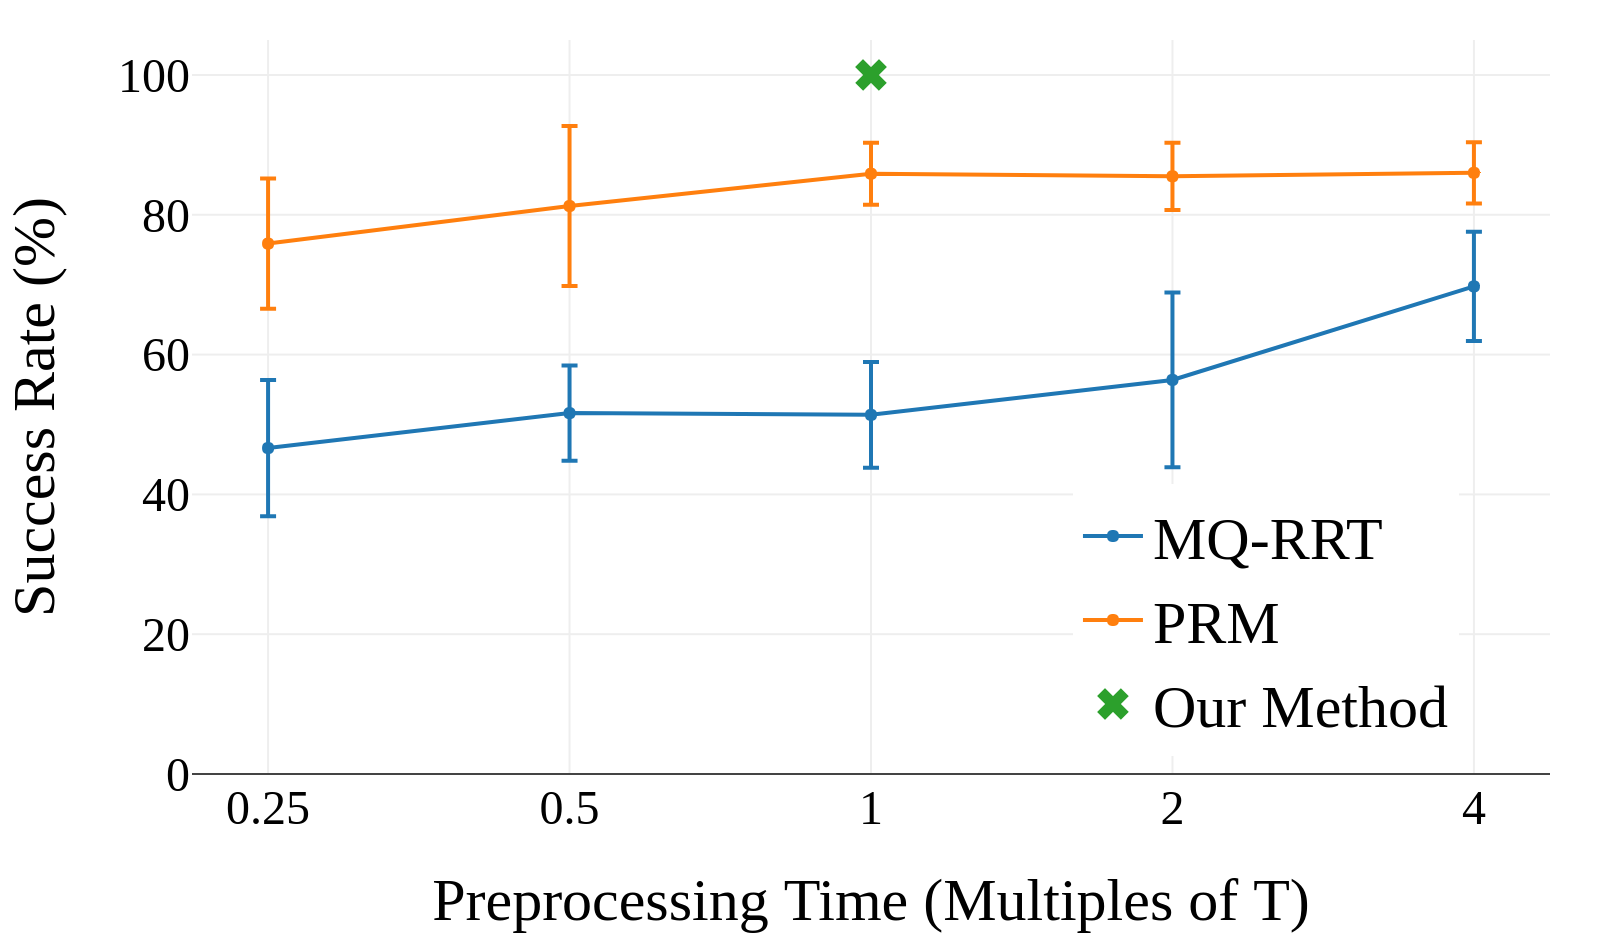
\includegraphics[width=0.9\linewidth]{success.png}
  \caption{}
  \label{fig:success}
\end{subfigure}
\hfill
\begin{subfigure}{0.5\textwidth}
\centering
  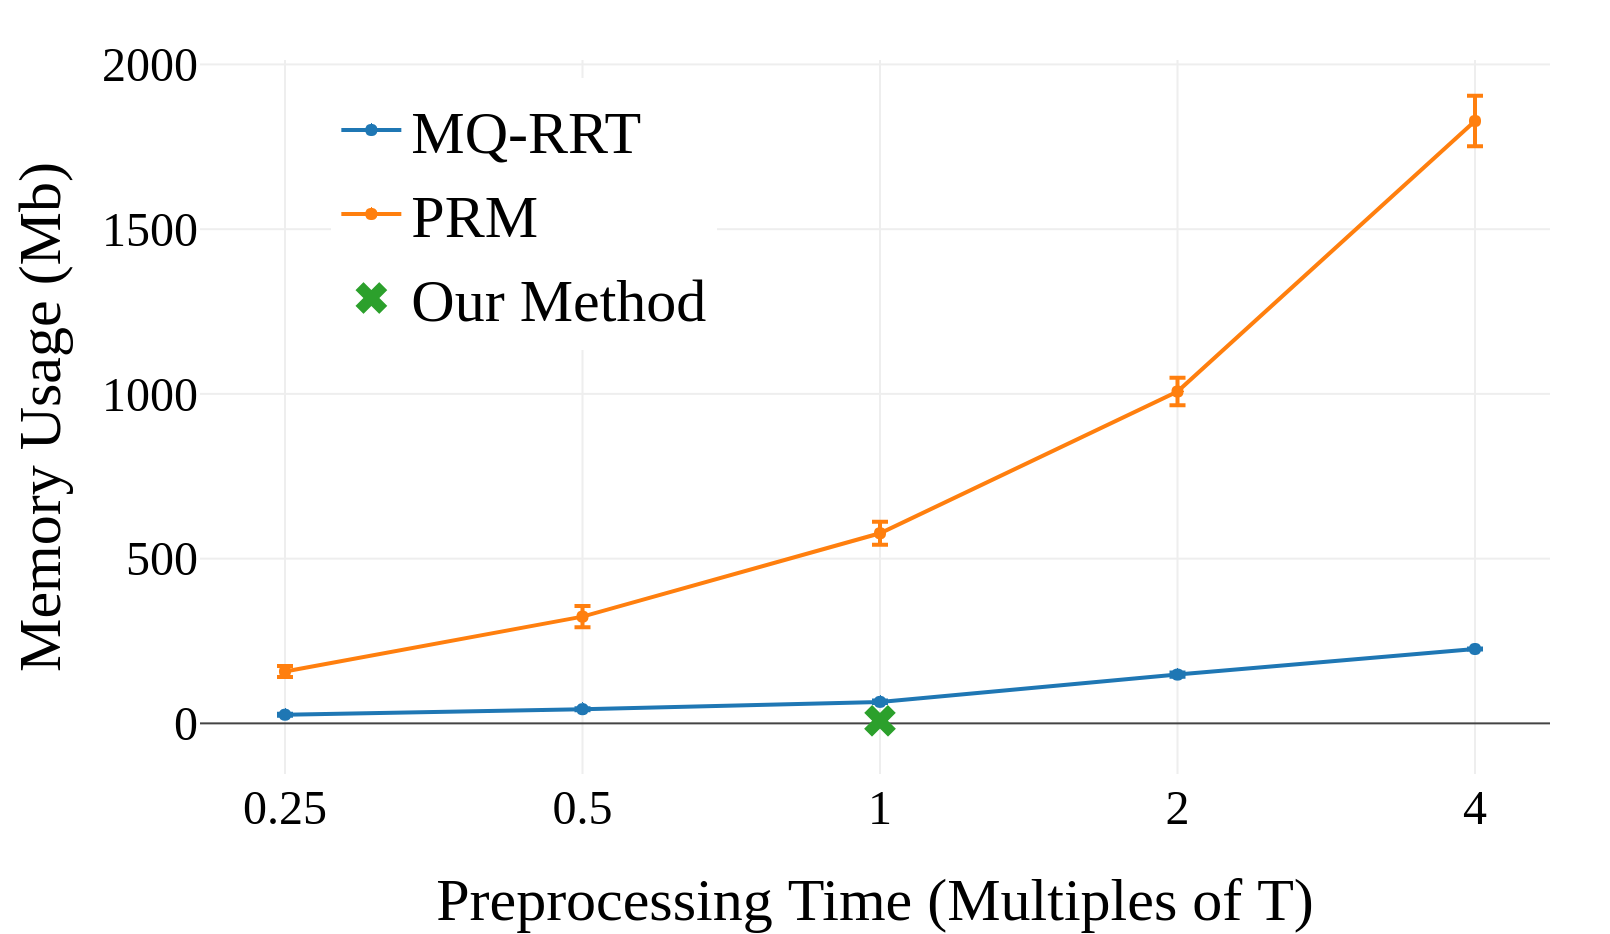
\includegraphics[width=0.9\linewidth]{memory.png}
  \caption{}
  \label{fig:memory}
\end{subfigure}
    \caption{Preprocessing time vs~(\subref{fig:success}) the success rates and~(\subref{fig:memory}) memory useage for the 200 queries averaged over 4 trials with different random number generation seeds for the PRM and the MQ-RRT algorithms. The results were computed at the intervals which are multiple of the time T = 1,455 seconds, that our method takes for precomputation. The green cross shows our method for reference.}
    \label{fig:plots}
\end{figure}

\subsection{Motion Planning for Truck-unloading Robot}
We tested our algorithm on an industrial truck-unloading robot~(see Fig.~\ref{fig:gmt}). The robot has a mobile omnidirectional base referred to as \textit{base} and two articulated mechanisms--a manipulator-like tool with suction grippers and a  scooper-like tool with conveyor belts, referred to as \textit{arm} and \textit{nose}, respectively. The general task of this robot is to unload boxes from delivery trucks as quickly and efficiently as possible and that is why it requires fast and reliable motion planning.

The robot's arm is 4-Dof and the nose has 3-Dof. We restrict the base motion to be one-dimensional and only allow the base to move either forward or backward. The robot can be controlled in different modes of operation and we tested our planner for each of these modes~(see table~\ref{tab:gmt}). The start state of the robot for each of these mode is a fixed configuration where the robot drops off the boxes or resets. Similar to the mail-sorting domain, the goal region is defined in the task space of the robot. For this robot we define two goal regions~$G_{\textrm{arm}}$ and~$G_{\textrm{nose}}$ for the arm and nose respectively. The discretization of~$G$ along position axes~($x,y,z$) is~0.05m and rotations axes~($\textit{roll, pitch, yaw}$) is 5 degrees. The sizes of the goal regions are selected as per the requirement of the task.
We compare our results with Weighted A* (WA*)algorithm. The results are summarized in Table~\ref{tab:gmt}. We observe our algorithm shows over an order of magnitude improvements in terms of planning times over the WA*. For a timeout of 5 seconds both the planners showed 100 percent success.

\begin{figure}
\centering
\includegraphics[width=\textwidth]{gmt.JPG}
    % \vspace{-2mm}
  \caption{
  Truck-unloader robot with its manipulator-like (arm) and scooper-like (nose) end effectors
}
    \label{fig:gmt}
% \vspace{-6mm}
\end{figure}

\begin{figure}
\centering
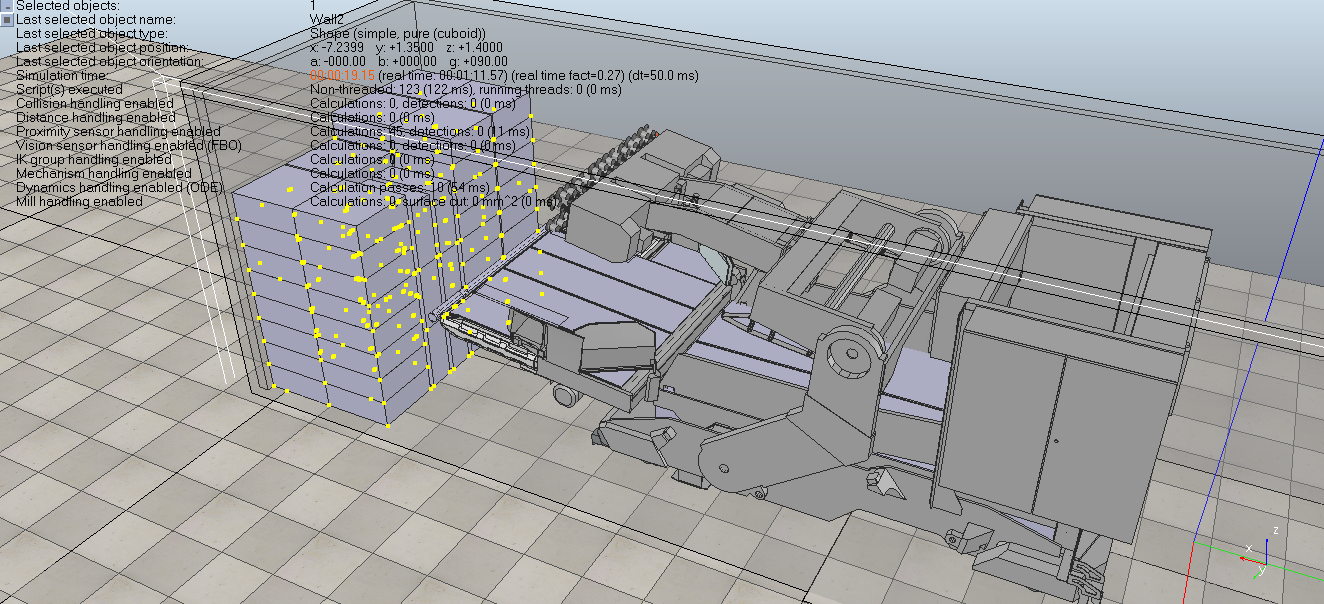
\includegraphics[width=\textwidth]{gmt_sim.png}
    % \vspace{-2mm}
  \caption{
  A simulated real world truck-unloading scenario
}
    \label{fig:gmt_sim}
% \vspace{-6mm}
\end{figure}

\begin{table*}[ht]
\centering
     \resizebox{0.7\columnwidth}{!}{%
    % \resizebox{1.4\textwidth}{!}{\begin{minipage}{\textwidth}
        \begin{tabular}{ l | c c c c}  
           & arm & nose & arm+base & nose+base\\
         \hline
         WA* 		& 12.8 & 7.2 & 7.5 & 4.4 \\
         Our Method & 0.69 & 0.29 & 0.5 & 0.47 \\
        \end{tabular}
    }
    \caption{Comparison of mean planning times~[ms] averaged over 100 randomized queries for different modes of operation of the truck-unloading robot. The number of subregions preprocessed for each of these modes~(left to right) are~101,~7,~85 and~308.}
    \label{tab:gmt}
  % \end{center}
% \vspace{-6mm}
\end{table*}

As this algorithm is only applicable to static (known) environments, we only preprocessed it with collision checking against the walls of the truck and with self collision checking and not with the boxes inside the truck. We also tested our planner in a simulated real world scenario~(see Fig.~\ref{fig:gmt_sim}) in conjunction with the WA* planner. For each query, we first ran our planner and validated the computed path against non-static obstacles i.e the boxes. We employed WA* as a fallback planner in case the first path is invalid. We observed that for all the queries ran for this scene, the fallback planner was never invoked. This experiment gave us an interesting use case for our planner to be employed in conjunction with conventional planners in the environments that are partially static.

\section{Algorithm Variant}
In this section we introduce a new variant of our algorithm and discuss its properties. The variant provides stronger constant-time guarantee for the case where the robot interleaves planning and execution. Specifically, it provides the same guarantee as lemma~\ref{lemma:o1} but without the included condition. We make the following high-level modifications to the previous algorithm to construct the new variant. 

\begin{enumerate}[label={\textbf{M\arabic*}},leftmargin=0.75cm]
\item \label{mod:flip} Flip the problem definition described in section~\ref{sec:pdef}. Namely instead of have a fixed start and a goal region, we have a fixed goal~$\sGoal$ and a start region~$S$~(see Fig.~\ref{fig:approach_flip}).
\item \label{mod:interleave} Interleave planning and execution and expand a constant number of states per action execution.
%\item \label{item:bound} Remove the bound~$\calD$ on the depth of the subregions.
\end{enumerate}

\begin{figure}
\centering
\includegraphics[width=\textwidth]{flip_version.pdf}
    % \vspace{-2mm}
  \caption{
  Visualization of approach. A discretized start region $S_\calS$ is shown. Subregions are depicted in green and the  obstacles are depicted in red.
  Precomputed paths from attractor states to~$\sGoal$ are depicted in blue.
 Given a query $(s_{\rm{start}}, s_{\rm{goal}})$, the returned path is given by the greedy path $\pi_g$~(depicted in purple) appended with the path~$\pi_i$ from~$\sAttract$ to $\sGoal$.
}
    \label{fig:approach_flip}
% \vspace{-6mm}
\end{figure}

The modifications result in the following lemma:
\vspace{2mm}
\begin{lemma}
\label{lemma:var:o1}
	Given the number of subregions~$|\calR|$ and the depth of the largest subregion~$\calD$, each action requires~$O(1)$ time delibration.
\end{lemma}

\begin{proof}
We consider the algorithm setting where~$|\calR|$ is bounded~(Assumption~\ref{asm:1:5}) but~$\calD$ is unbounded. From lemma~\ref{lemma:unboundedD} thereby, the query phase can find path in~$O(|\calR|)$ time.
%
However by modification~\ref{mod:interleave}, by interleaving planning and execution, the algorithm requires~$O(1)$ planning time per action.
%The completeness guarantee follows from section~\ref{sec:analysis} and by the construction of the algorithm, it is guaranteed that a state is never re-expanded or re-visited by the robot.
Once the robot reaches~$\sAttract$, it can then continue to follow the pre-stored path~$\pi_i$. 
\end{proof}

\textbf{CTMP Criteria:} We now analyse the algorithm variant under the CTMP criteria described in chapter~\ref{sec:ctmp}. Since the algorithm requires~$O(1)$ time to plan the next action, $T_\textrm{const} (< \Tbound)$ is constant-time bounded.
%
Furthermore, Lemma~\ref{lemma:greedy} assures that the greedy path~$\pi_g$ does not contain cycles, otherwise the greedy search would be incomplete. Hence from lemmas~\ref{lemma:var:o1} and~\ref{lemma:greedy} and by Def.~\ref{def:complete} we have the following theorem:

\vspace{2mm}
\begin{theorem}
	The algorithm variant is CTMP-Complete.
%	By Def.~\ref{ctmp:def} and from lemmas~\ref{lemma:o1} and~\ref{lemma:greedy}, the algorithm is a CTMP algorithm.
\end{theorem}

We also have the following corollary.

\vspace{2mm}
\begin{cor}
	The algorithm variant can be used for non-stop execution under the condition~$\Tconst < \Texec$
\end{cor}

Note that flipping the problem definition~(\ref{mod:flip}) will change the set of domains that our approach is applicable to. The experimental evaluation of this algorithm variant is outside the scope of this thesis and left as future work.

\newpage
\chapter{CTMP for Conveyor-pickup Task}
\label{chap:rss}
\section{Overview}
Conveyor belts are widely used in automated distribution, warehousing, as well as for manufacturing and production facilities. In the modern times robotic manipulators are being deployed extensively at the conveyor belts for automation and faster operations~\cite{zhang2018gilbreth}. In order to maintain a high-distribution throughput, manipulators must pick up moving objects without having to stop the conveyor for every grasp. In this work, we consider the problem of motion planning for grasping moving objects off a conveyor. An object in motion imposes a requirement that it should be picked up in a short window of time. The motion planner for the arm, therefore, must compute a path within a bounded time frame to be able to successfully perform this task.

\begin{figure}[t]
    \centering
    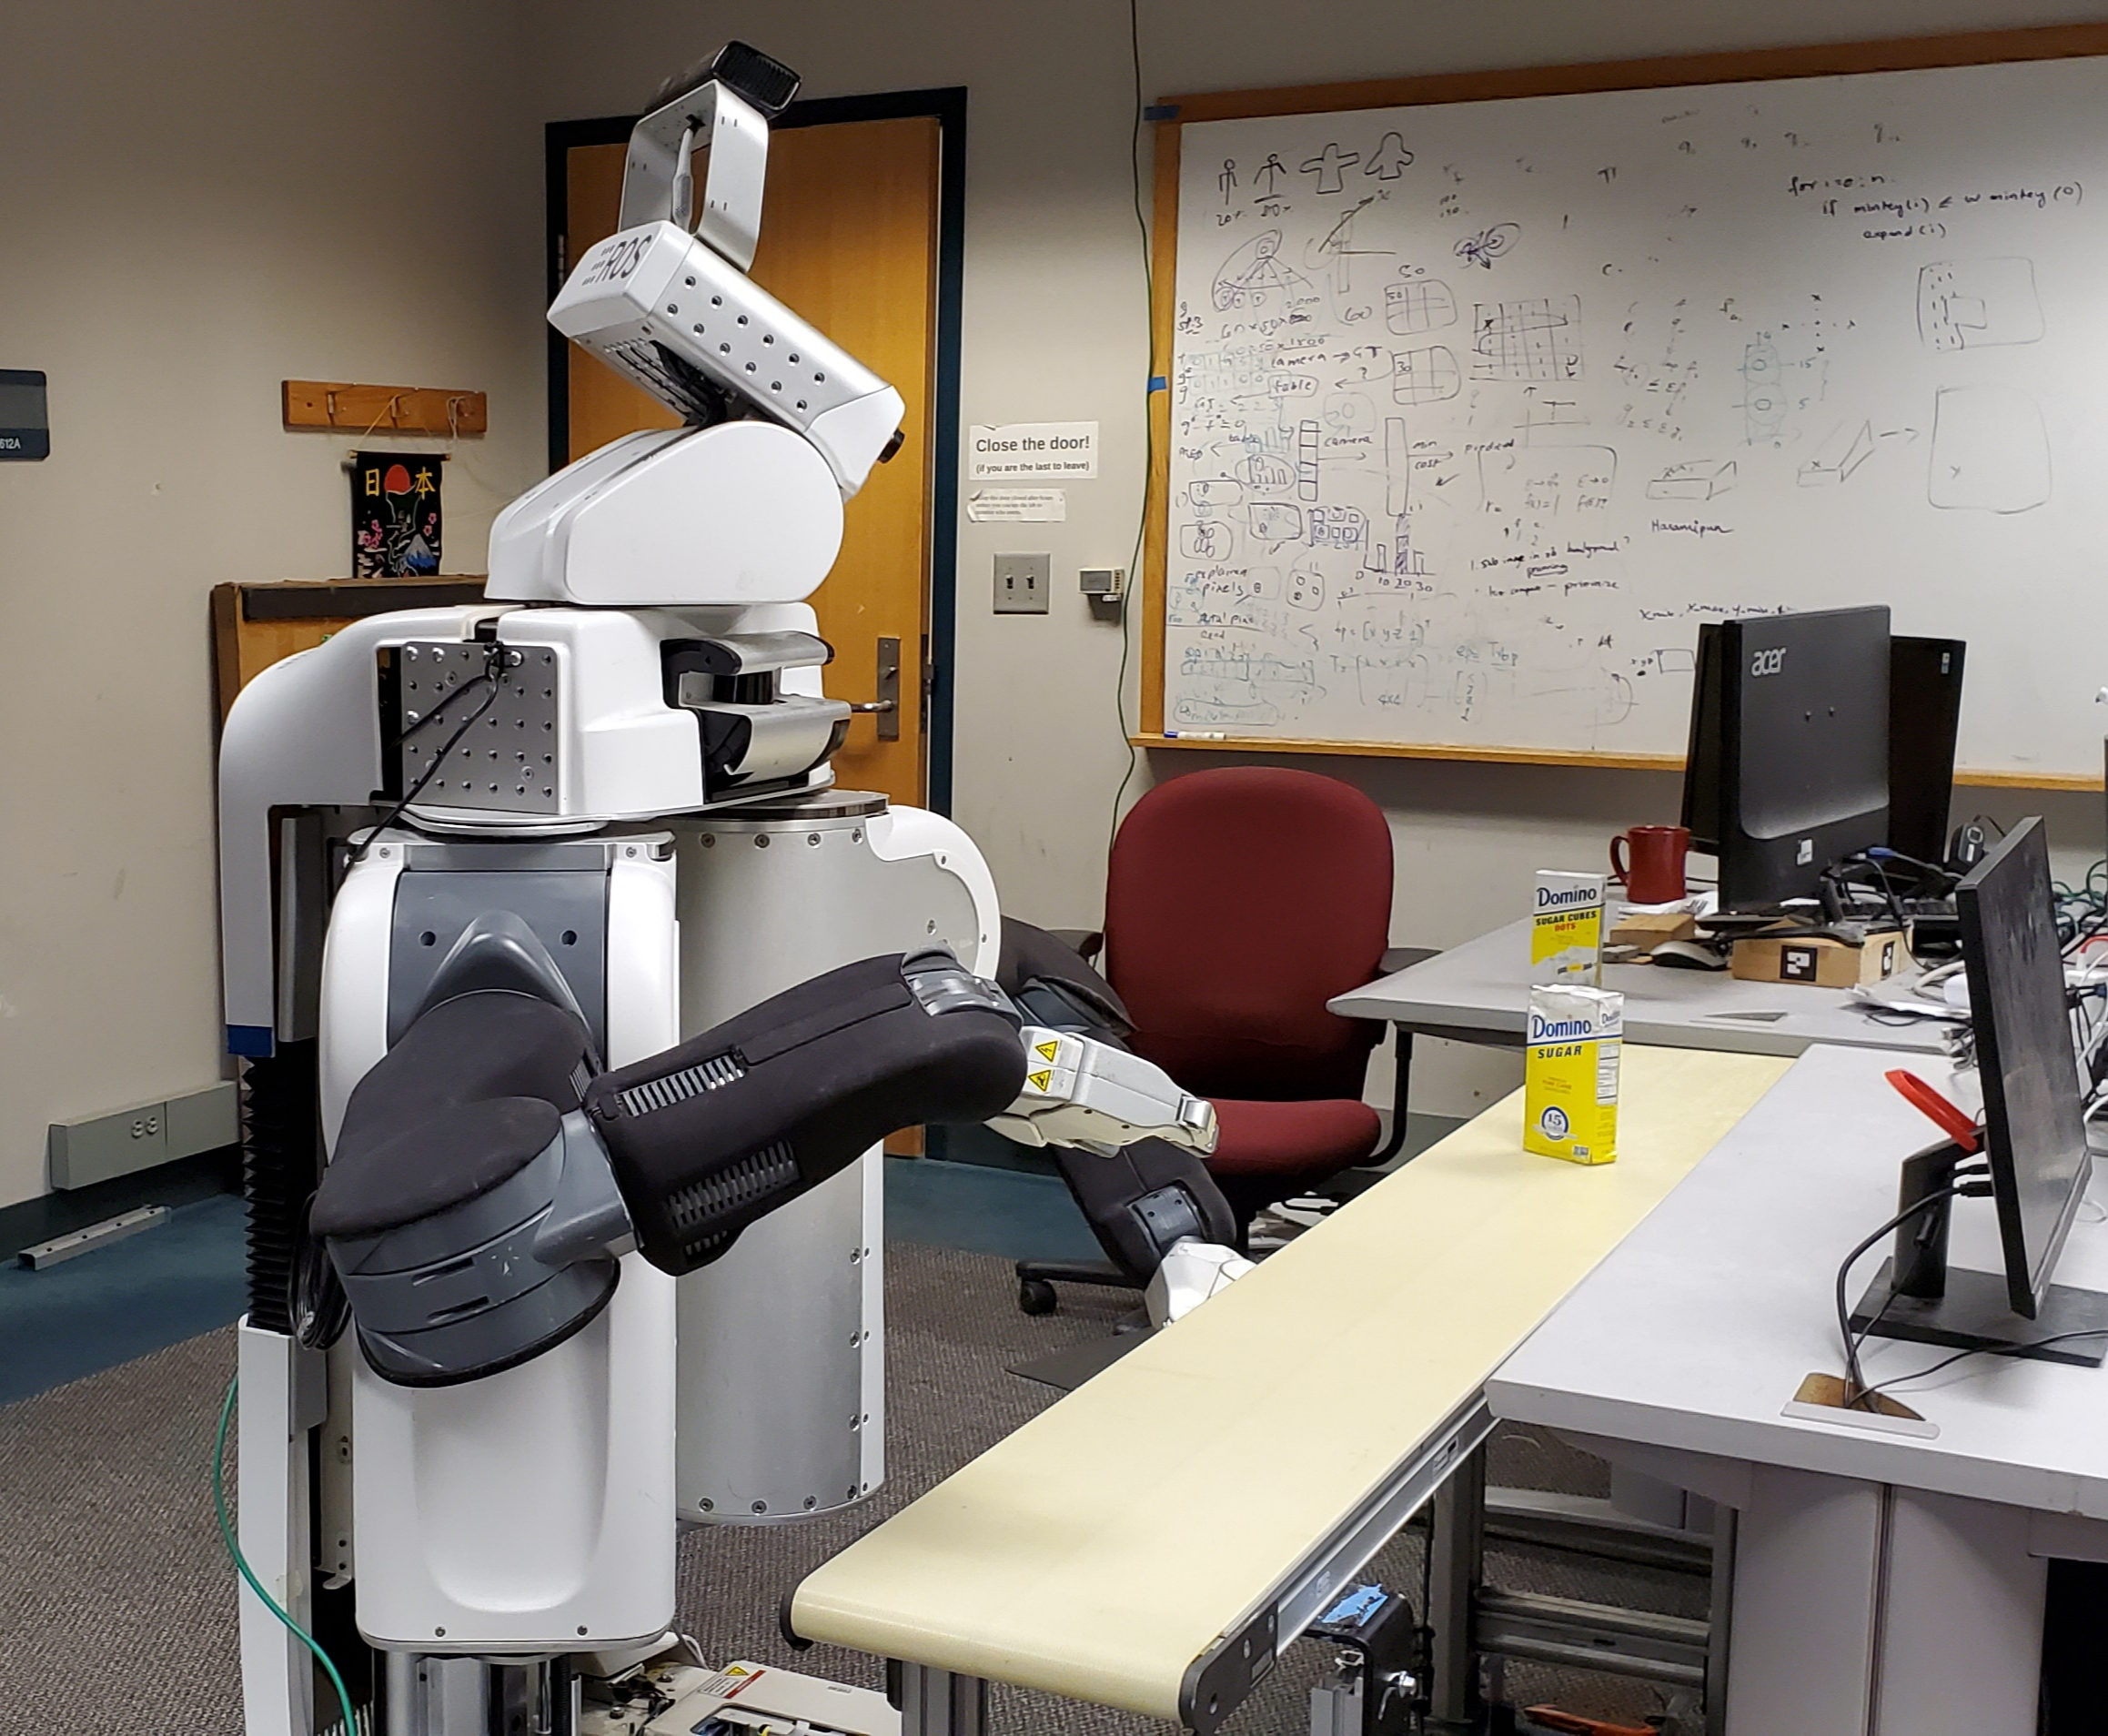
\includegraphics[trim=0 50 0 100, clip, width=\columnwidth]{figs/cover_pic.jpg}
    \caption{
    \CaptionTextSize
    A scene demonstrating the PR2 robot picking up a moving object (sugar box) off a conveyor belt.}
    \label{fig:intro_pic}
\end{figure}

Manipulation relies on high quality detection and localization of moving objects. When the object first enters the robot's field of view, the initial perception estimates of the object's pose are often inaccurate. Consider the example of an object (sugar box) moving along the conveyor towards the robot in Fig.~\ref{fig:intro_pic}, shown through an image sequence as captured by the robot's Kinect camera in Fig.~\ref{fig:pose_sequence}. 
%
The plot in Fig.~\ref{fig:pose_sequence} shows the variation of the error between the filtered input point cloud and a point cloud computed from the predicted pose from our Iterative Closest Point (ICP)-based perception strategy~\cite{ISL19} as the object gets closer to the camera. We observe that the error decreases as the object moves closer, indicating that the point clouds overlap more closely due to more accurate pose estimates closer to the camera.
%ijrr
In a real world set up, instead of relying on onboard sensing, the environment could be instrumented with multiple sensors to get a more accurate pose. Even then, for tracking purposes, typically, multiple frames are acquired and filtered to get a more accurate estimate.

However, if the robot waits too long to get an accurate estimate of the object pose, the delay in starting plan execution could cause the robot to miss the object. The likelihood of this occurring increases as the speed of the conveyor increases. Therefore, the robot should start executing a plan computed for the initial pose and as it gets better estimates, it should repeatedly replan for the new goals. However, for every replanning query, the time window for the pickup shrinks. This makes the planner's job difficult to support real-time planning.


%% why problem is hard
Furthermore, the planning problem is challenging because the motion planner has to account for the dynamic object and thus plan with time as one of the planning dimensions. It should generate a valid trajectory that avoids collision with the environment around it and also with the target object to ensure that it does not damage or topple it during the grasp. Avoiding collisions with the object requires precise geometric collision checking between the object geometry and the geometry of the manipulator.
The robot arms also have kinodynamic constraints such as torque and velocity limits that the motion planner may have to account for while computing the plans, especially when the robots must move at high speeds.
The resulting complexity of the planning problem makes it infeasible to plan online for this task.

%%
Motivated by these challenges, we propose an algorithm that leverages offline preprocessing to provide bounds on the planning time when the planner is invoked online. Our key insight is that in our domain the manipulation task is highly repetitive. Even for different object poses, the computed paths are quite similar and can be efficiently reused to speed up online planning. Based on this insight, we derive a method that precomputes a representative set of paths with some auxiliary datastructures offline and uses them online in a way that provides \emph{constant-time planning guarantee}.
We present it as an instance of a new class of algorithms which we call Constant-time Motion Planning (CTMP) algorithms.
To the best of our knowledge, our approach is the first to provide constant-time planning guarantee on generating motions for indefinite horizons i.e. all the way to the goal.
%for a dynamic environment.

%
We experimentally show that constant-time planning and replanning capability is necessary for a successful conveyor pickup task. Specifically if we only perform one-time planning, that is planning only once either for the very first and potentially inaccurate pose estimate or for a delayed but accurate pose estimate of the object, the robot frequently fails to pick the object.
\begin{figure}[t]
    \centering
    \begin{subfigure}{.49\textwidth}
    %   \centering
        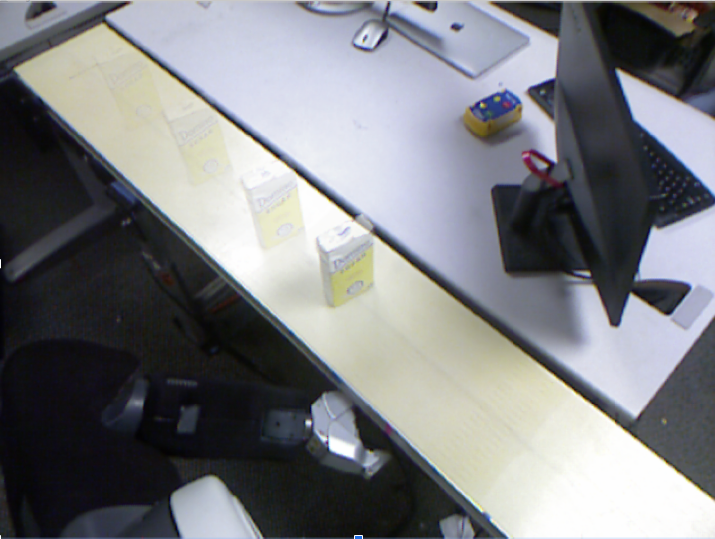
\includegraphics[width=\textwidth]{object_blur}
        \caption{}
        \label{fig:obj1}
    \end{subfigure}
    \begin{subfigure}{0.49\textwidth}
    %   \centering
        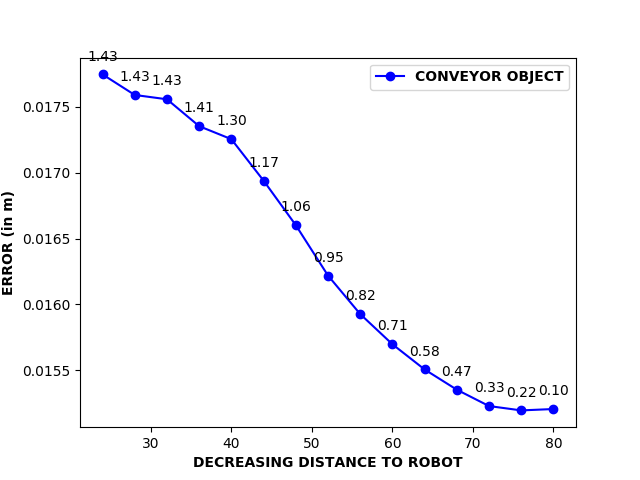
\includegraphics[width=\textwidth]{pose_error_plot}
        \caption{}
        \label{fig:obj2}
    \end{subfigure}
    \caption{
    \CaptionTextSize
    (\subref{fig:obj1})~Depiction of an object moving along a conveyor towards the robot.
    %
    (\subref{fig:obj2})~Pose error as a function of the distance from the conveyor's start. Specifically we use ADD-S error \cite{add_metric},
    calculated as the average pair wise minimum distance between the input point cloud and the point cloud corresponding to the predicted pose.
    }
    \label{fig:pose_sequence}
\end{figure}

\section{Algorithmic framework}
\subsection{Problem Setup}
Our system is comprised of 
a robot manipulator,
a conveyor belt moving at some known velocity,
a set of known objects~$\calO$ that need to be grasped and 
a perception system that is able to estimate the type of object and its location on the conveyor belt. Here, we assume that the geometric models of the target objects are known apriori and we are given a set of feasible grasps for each object~$o \in \calO$.

Given a pose $g$ of an object $o \in \calO$, our task is to plan the motion of the robot such that it grasps~$o$ from the conveyor belt at some future time.
%
Unfortunately, the perception system may give inaccurate object poses.
Thus, the pose $g$ will be updated by the perception system as the robot is executing its motion. 
To allow for the robot to move towards the updated pose in real time, we introduce the additional requirement that planning should be done within a user-specified time bound~\Tbound.
%
For ease of exposition, when we say that we plan to a pose $g$ of $o$ that is given by the perception system, 
we mean that we plan the motion of the robot such that it will be able to pick~$o$ from the conveyor belt at some future time. 
This is explained in detail in Sec.~\ref{sec:robot_results} and in Fig.~\ref{fig:pe}.

%
We denote by $\Gfull$ the discretized set of initial object poses on the conveyor belt that the perception system can perceive.
%
Finally, we assume that the robot has an initial state \Shome corresponding to the time $t=0$ from which it starts planning to grasp any object.


Roughly speaking, the objective is to enable planning and replanning to any goal pose $ g \in \Gfull$ in bounded time~\Tbound regardless of the robot's current state.
%More specifically, the perception system is setup such that it sends updated pose estimates on the fly as the object moves along the conveyor belt and as the robot approaches the object. %  
%
% To formalize this idea, let us introduce the notion of \emph{reachable} and \emph{covered} states:
%
% \begin{definition}
%     A goal pose $g \in \Gfull$ is said to be \emph{reachable} from a state $s$ if there exists a path from $s$ to $g$ and it can be computed in finite time.
% \end{definition}
%
% \begin{definition}
%     A reachable pose $g \in \Gfull$ is said to be \emph{covered} by a state $s$ if 
%     the planner can find a path from $s$ to $g$ within time~\Tbound.
% \end{definition}
%
Specifically we aim to develop a CTMP-complete algorithm, so that 
for any state $s$ that the system can be in 
and every reachable goal pose $g \in \Gfull$ from $s$ updated by the perception system,
$g$ is covered by $s$.

\ignore{
We are now ready to state the assumptions for which we can solve the problem defined.
%\begin{definition}
%    A goal region $G \subseteq \Gfull$ is said to be \emph{reachable} from a state $s$ if any state $g \in G$ is reachable from $s$.
%\end{definition}

%We make the following assumptions about the system.
\begin{enumerate}[label={\textbf{A\arabic*}},leftmargin=0.75cm]
    % \item \label{assum:1} The goal set \Gfull is reachable from the start state~\Shome. Namely,  $G^{\rm reach}(\Shome) = \Gfull$.
    
\ignore{
    \item \label{assum:2} Given a path 
    $\Pi = \{s_0, \ldots, s_k \}$ 
    s.t. $s_0 = \Shome$ and $s_k \in \Gfull$, 
    we have that $G^{\rm reach}(s_{i+1}) \subset G^{\rm reach}(s_{i})$.
    Namely, the reachable set of goals for a state on the path is a subset of the reachable set of every other state on that path that exists before it.
    \os{Oren - Didn't we agree that this is not an assumption but a property?}
}

%    \item \label{assum:3} \Gfull would accommodate for an error $\epsilon$ in the initial pose estimate $g_{\textrm{init}}$ of the perception system. Each subsequent estimate $g_{\textrm{next}}$ will be within the $\epsilon$ window around $g_{\textrm{init}}$ (in retrospect because the conveyor is moving).
    \item \label{assum:4} There exists a replan cutoff time $t=\Trc$, after which the planner does not replan and continues to execute the last planned path.

    \item \label{assum:5} For any time $0 \leq t \leq \Trc$, the environment is static. Namely, objects on the conveyor belt cannot collide with the robot during that time.

    \item \label{assum:3} The pose estimation error of the perception system is bounded by a distance~$\varepsilon$.
        
%    \item \label{assum:3} Given an initial goal pose $g_{\textrm{init}} \in \Gfull$ by the perception system, any subsequent pose $g_{\textrm{new}} \in \Gfull$ is at most $\varepsilon$ distance away from $g_{\textrm{init}}$ (after accounting for the fact that the object moved along the conveyor belt).
\end{enumerate}
Assumptions~\ref{assum:4}-\ref{assum:5} enforce a requirement that the perception system must converge on an accurate estimate $g$ before \Trc, and until \Trc, $o$ is guaranteed to be at a safe distance from the robot.
%
Assumption~\ref{assum:3} bounds the maximum error of the perception system and is explained in detail in Sec.~\ref{sec:eval} and in Fig.~\ref{fig:pe}
% Assumption~\ref{assum:1} corresponds to properties of the environment \emph{without} taking the objects on the conveyor belt into account 
% while


% Assumptions~\ref{assum:3}-\ref{assum:5} correspond to properties of the environment that account for the perception system and the objects on the conveyor belt.
}
%ijrr
We assume that the pose estimation error of the perception system is bounded by a distance~$\varepsilon$ at a given conveyor belt's speed. The details related to this are provided in Sec.~\ref{sec:goal_region}
We also specify a replan cutoff time $t=\Trc$ after which the planner does not replan and continues to execute the last planned path until the goal is reached. The time~$\Trc$ could be chosen based on when the perception system is expected to send an accurate pose estimate, and therefore no replanning is needed from there on.


%\section{Algorithmic framework}
\subsection{Straw man approach}
\label{subsec:strawman}
Our approach for constant-time planning relies on a \emph{preprocessing} stage that allows to efficiently compute paths in a \emph{query} stage to any goal.
% (under Assumptions~\ref{assum:4}-\ref{assum:3}). 
%
Before we describe our approach, we start by describing a \naive method that solves the aforementioned problem but requires a prohibitive amount of memory.
%
This can be seen as a warmup before describing our algorithm which exhibits the same traits but does so in a memory-efficient manner.

\begin{figure*}[t]
    \centering
    % \hspace{3mm}
    \begin{subfigure}{.49\textwidth}
    %   \centering
        % \includegraphics[trim=0 0 40 0, clip,width=0.9\textwidth]{naive1}
        \includegraphics[width=0.9\textwidth]{naive1}
        \caption{}
        \label{fig:naive1}
    \end{subfigure}
    %\hfill
    \begin{subfigure}{0.49\textwidth}
    %   \centering
        % \includegraphics[trim=0 0 15 0, clip,width=0.9\textwidth]{naive2}
        \includegraphics[width=0.9\textwidth]{naive2}
        \caption{}
        \label{fig:naive2}
    \end{subfigure}
    \caption{
    \CaptionTextSize
    The figures show paths discretized from timesteps $t_0$ to~$\Trc$ with steps of size $\delta_t$.
    (\subref{fig:naive1})~At $t_0$, the algorithm computes~$n_{\rm goal}$ paths, from~\Shome to every $g \in \Gfull$.
    (\subref{fig:naive2})~At $t_1 = \delta_t$, the algorithm computes~$n_{\rm goal}^2$ paths, from all $n_{\rm goal}$ replanable states at $t_1$ to every $g \in \Gfull$ (here we only show paths from three states).
    Thus, the number of paths increases exponentially at every timestep.
    }
    \label{fig:naive}
\end{figure*}

We first compute from \Shome a path $\pi_g$ to every reachable $g \in \Gfull$. 
%(such a path exists following \ref{assum:1}).
These paths can be stored in a lookup (hash) table which can be queried in constant time \Tconst (assuming perfect hashing~\cite{czech1997perfect}).
For the straw man approach, since there is no utility of having a \Tbound larger than \Tconst as it only performs look up operations at query time, we have $\Tbound = \Tconst$.
By storing paths to all the goals, every goal is covered by \Shome and this allows us to start executing a path once the perception system gives its initial pose estimate.
However, we need to account for pose update while executing~$\pi_g$. 
%
% Following \ref{assum:4} and \ref{assum:5},
This only needs to be done up until time~\Trc, since no future improved estimates are expected from the perception system.
Thus, we discretize each path uniformly with resolution $\delta_t$.
%As we will see, this will allow the system to start executing a new path within $\Tbound + \delta_t$ after a new pose estimation is obtained from the perception system.
%
We call all states that are less than \Trc time from \Shome \emph{replanable states}.


Next, for every replanable state along each path $\pi_g$, we compute a new path to all goals. 
%\bound{that are $\varepsilon$ away from $g$}.
%See Fig.~\ref{fig:naive}.
%
This will ensure that all goals are covered by all replanable states. Namely, it will allow to immediately start executing a new path once the goal location is updated by the perception system.
%
Unfortunately, the perception system may update the goal location more than once. Thus, this process needs to be performed recursively for the new paths as well.


The outcome of the preprocessing stage is a set of precomputed collision-free paths starting at states that are at most $\Trc$ from \Shome and end at goal states.
The paths are stored in a lookup table $\calM: S \times \Gfull \rightarrow \{ \pi_1, \pi_2, \ldots \}$ that can be queried in $\Tbound=\Tconst$ time to find a path from any given $s \in S$ to $g \in \Gfull$.
% \OS{$S$ is formally defined in IV.C...}


In the query stage we obtain an estimation $g_1$ of the goal pose by the perception system. 
The algorithm then retrieves the path~$\pi_1(\Shome,g_1)$ (from~\Shome to~$g_1$) from $\calM$ and the robot starts executing~$\pi_1(\Shome,g_1)$.
%
For every new estimation $g_i$ of the goal pose obtained from the perception system while the system is executing path $\pi_{i-1}(s_{i-1},g_{i-1})$, the algorithm retrieves from $\calM$ the path $\pi_i(s_i,g_i)$ from the nearest state~$s_i$ along $\pi_{i-1}(s_{i-1},g_{i-1})$ that is least $\Tbound$ away from~$s_{i-1}$. The robot then starts executing~$\pi_i(s_i,g_i)$ once it reaches~$s_i$.
Hence, the straw man algorithm is trivially a CTMP-complete algorithm.

Clearly, every possible goal is covered for every possible configuration that the robot might be in during execution by this brute force approach, however it requires a massive amount of memory and prepreprocessing time.
Let $n_{\rm goal} = \vert \Gfull \vert$ be the number of goals and
$\ell$ be the number of states between \Shome and the state that is \Trc time away.
This approach requires precomputing and storing $O(n_{\rm goal}^\ell)$ paths which is clearly infeasible (see Fig.~\ref{fig:naive}).
In the next sections, we show how we can dramatically reduce the memory footprint of the approach without compromising on the system's capabilities.




\subsection{Algorithmic approach}
While the straw man algorithm presented  allows for planning to any goal pose $ g \in \Gfull$ within \Tconst time, its memory footprint is prohibitively large.
%
We suggest to reduce the memory footprint by building on the observation that many paths to close-by goals traverse very similar parts of the configurations space. Instead of generating a plan strictly within $\Tconst$ time, our approach trades off preprocessing efforts with the bound on the planning time and guarantees to generate a solution within the user-specified time bound $\Tbound (> \Tconst)$.

%Similar to the straw man algorithm, our preprocessing stage runs in two steps.
%In the first step we  compute from \Shome a path $\Pi_g$ to every goal $ g \in \Gfull$. However, this is done by computing a set of so-called ``root paths'' $\{\Pi_1, \ldots, \Pi_k \}$ from \Shome to a subset of goals in \Gfull (here we will have that $k \ll n_{\rm goal})$.

The key idea of our approach is that instead of computing (and storing) paths to all reachable goals in \Gfull, we compute a relatively small subset of so-called ``root paths" that can be reused in such a way that we can still cover \Gfull fully. Namely, at query time, we can reuse these paths to plan to any $g\in \Gfull$ within \Tbound. The idea is illustrated in Fig.~\ref{fig:crp}.


First, we compute a set of root paths $\{\Pi_1, \ldots, \Pi_k \}$ from~\Shome to cover~\Gfull by \Shome (here we will have that $k \ll n_{\rm goal})$ 
%
Next, for all replanabale states along these root paths, the algorithm recursively computes additional root paths so that their reachable goals are also covered.
%However, this is done by attempting to re-use previously-computed root paths which, in turn, allows for a very low memory footprint.
During this process, additional root paths are computed only when the already existing set of root paths does not provide enough guidance to the search to cover \Gfull i.e., to be able to compute a path to any $g \in \Gfull$ within \Tbound.
%
%It is important to note that replanable states are not only the ones that lie on the root paths from \Shome---whenever the recursion happens we compute a new set of root paths and generate new replanable states
%
The remainder of this section formalizes these ideas.

\subsection{Algorithmic building blocks}
\label{subsec:alg_building_blocks}
We start by introducing the algorithmic building blocks that we use.
Specifically, we start by describing the motion planner \calP  that is used to compute the root paths 
and then continue to describe how they can be used as \emph{experiences} to efficiently compute paths to other goals.
We implemented two types of motion planners. One operates in a time-configuration space and the other is a kinodynamic motion planner that plans with additional state dimensions of joint velocities in order to satisfy the kinodynamic constraints of the robot. While the former planning framework is simpler and works successfully on a physical robot in our experiments, the latter might be more desirable for operating a robot closer to its maximum performance limits.
% \subsubsection{Motion planner}

We use a heuristic search-based planning approach with motion primitives (see, e.g,~\cite{CCL10,CSCL11,LF09})
as it allows for deterministic planning time which is key in our domain.
% Moreover, such planners can easily handle under-defined goals as we have in our setting.
%ijrr
Moreover, such planners can conveniently handle under-defined goals; goals that can have many solutions.
For instance, the goal representation does not include the time dimension which allows the robot to pick up the object at any position along the conveyor belt. 
We define a goal as a grasp pose for the goal object. The grasp pose for a target object $o$ is manually selected.
%ijrr
% while the planning dimension includes the DoFs of the robot as well as the time dimension.
\subsubsection{Time-Configuration Motion Planner}
\hfill\\
\textbf{State space and graph construction.}
We define a state~$s$ as a pair $(q,t)$ where $q = (\theta_1, ..., \theta_n)$ is a configuration represented by the joint angles for an $n$-DOF robot arm (in our setting $n=$7) and $t$ is the time associated with $q$.
%
Given a state~$s$ we define two types of motion primitives which are short kinodynamically-feasible motions that the robot can execute.
%The first, which we term \emph{predefined} primitives are used to move to a pre-grasp position while the second, termed \emph{dynamic} primitives are used to perform grasping after the robot reached a pre-grasp position.
%

The first type of motion primitives are predefined primitives. These are small individual joint movements in either direction as well as \emph{wait} actions.
These primitives have non-uniform resolution. For each joint, we define two  motion primitives of distance $\pm$4$^{\circ}$. In addition, for the first four of the seven robot joints we define  two additional  primitives each, of distance $\pm$7$^{\circ}$. We only allow moving one joint at a time which makes it a total of 23 predefined primitives.
For each motion primitive, we compute its duration by using a nominal constant velocity profile for the  joint that is moved.
%\footnote{Computing a plan using these motion primitives is not guaranteed to respect the acceleration limits of the robot. However, in practice this seldom occurs and we elaborate in Sec.~\ref{sec:eval} how we handle these execution errors.}.
%

The second type of primitives are dynamic primitives. They are generated by the search only at the states that represent the arm configurations where the end effector is close to the object. These primitives correspond to the actual grasping of the object while it is moving.
The dynamic primitives are generated by using a Jacobian pseudo inverse-based control law similar to what~\cite{menon2014motion} used. 
The desired velocity of the end effector is computed for which the end-effector minimizes the distance to the grasp pose. Once the gripper encloses the object, it moves along with the object until the gripper is closed. Some examples of the dynamic primitives are shown in Fig.~\ref{fig:amp}. During the search, all motion primitives are checked for validity with respect to collision and joint limits.
%Additional details omitted due to lack of space. 

\begin{figure}[t]
    \centering
    % \hspace{3mm}
    % \begin{subfigure}{.35\textwidth}
        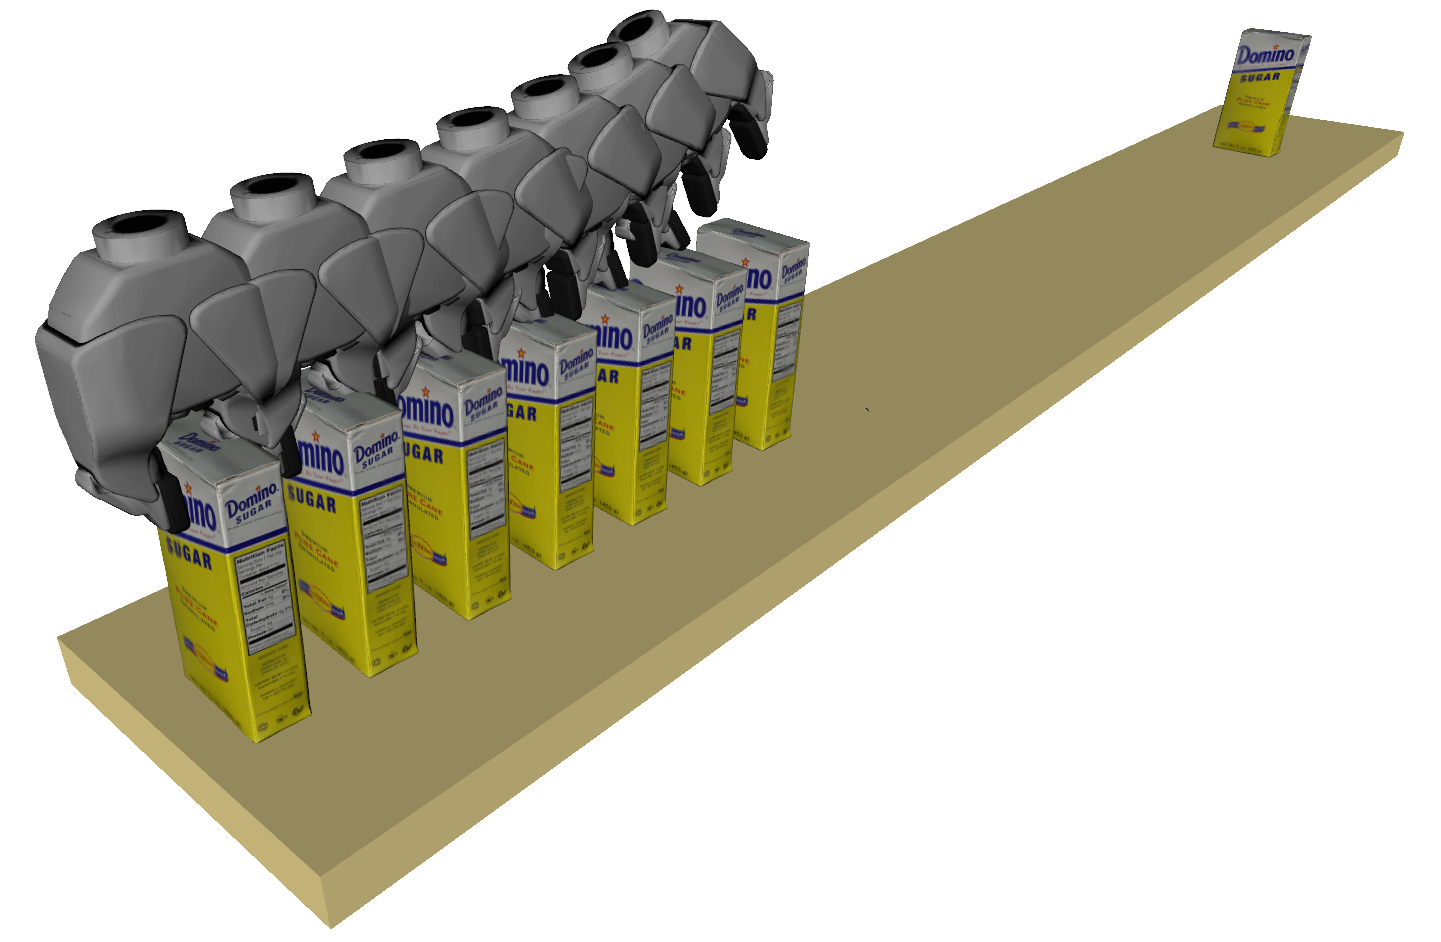
\includegraphics[width=0.48\textwidth]{amp1.png}
    % \end{subfigure}
    %\hfill
    % \begin{subfigure}{0.35\textwidth}
        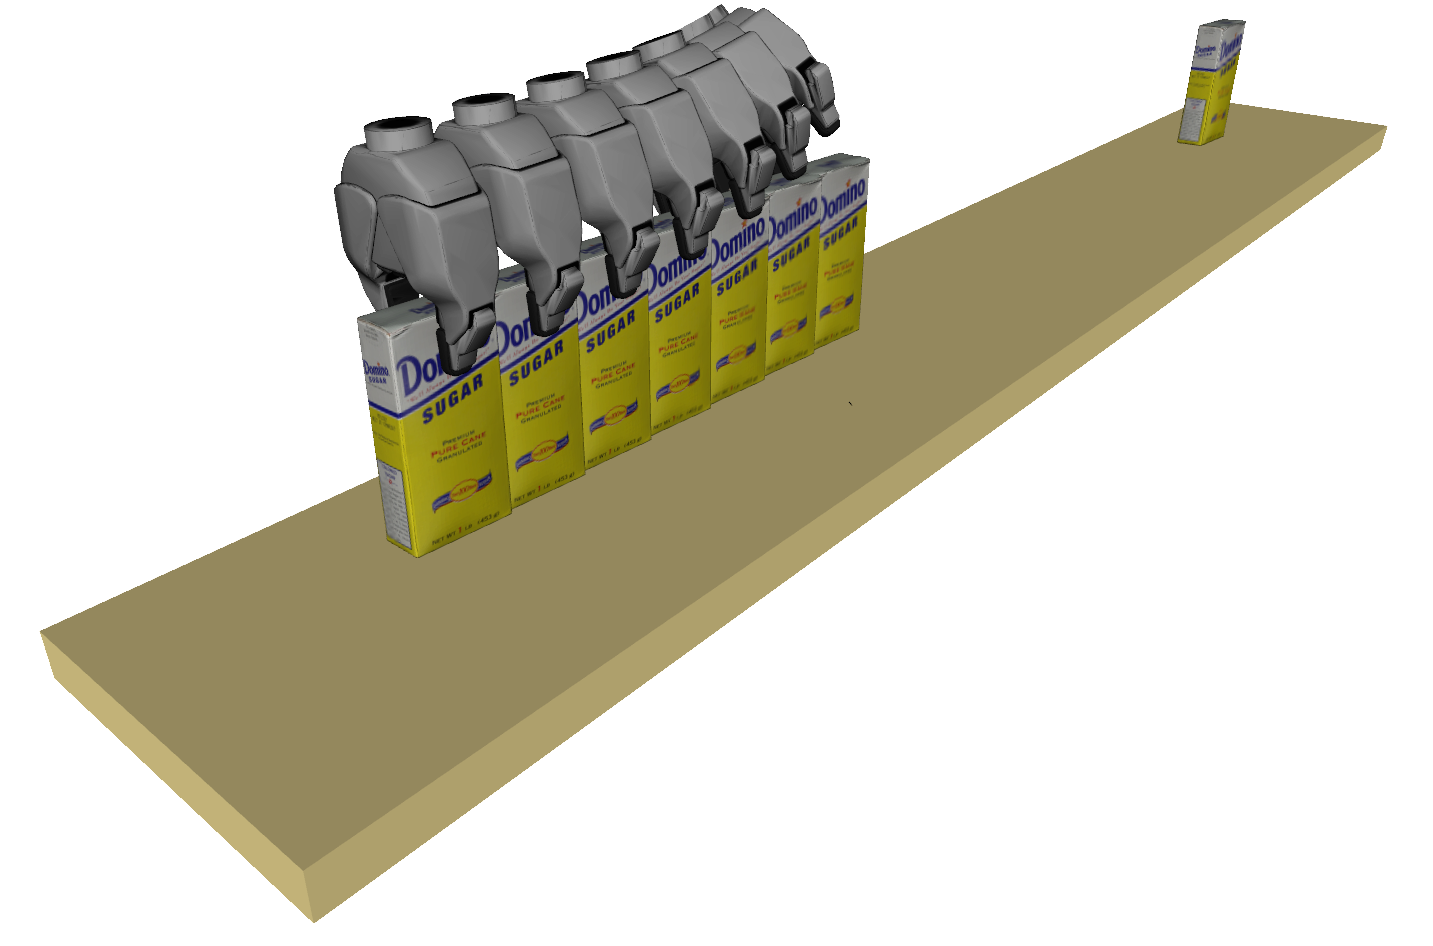
\includegraphics[width=0.48\textwidth]{amp2.png}
    % \end{subfigure}
    \caption{
    The figures show the dynamic motion primitive for two different initial poses of the sugar box. (Only the gripper poses are visualized.) The sugar box shown at the rear of the conveyor belt in the examples depicts its initial pose.
    }
    \label{fig:amp}
\end{figure}

\textbf{Heuristic Function}
The graph search is guided by an efficient and fast-to-compute heuristic function which in our case has two components.
The first component drives the search to intercept the object at the right time and 
the second component guides the search to correct the orientation of the end effector as it approaches the object. 
Mathematically, our heuristic function is given by
\begin{equation} \label{eq:h1}
 h(s,g) = \max (\Delta t(s,g), \lambda \cdot \textsc{AngleDiff}(s,g)).
\end{equation}
Here, $\Delta t(s,g)$ is the expected time to intercept the object which can be analytically computed from the positions of the target object and the end-effector, the velocity of the target object and the speed of the end-effector. We pick a nominal speed for the end-effector to solve the problem. \textsc{AngleDiff}($s,g$) gives the magnitude of angular difference between the end-effector's current pose and the grasp pose. The coefficient $\lambda$ is used as a weighting factor.

% ijrr
We manually define the grasps for the target object. In our experiments, we use a single grasp as can be seen in Fig.~\ref{fig:amp}. However, the planner can also use a set of grasps by trying out each grasp from the set until it succeeds. This would potentially increase the number of reachable goals for the CTMP algorithm.
%% kinodynamic
\subsubsection{Kinodynamic Motion Planner}
\hfill\\
The time-configuration motion planner does not guarantee that the plan when transformed into a trajectory will satisfy robot's torque limits. To this end, we extend the previous motion planner framework to be able to plan within the kinodynamic constraints of the robot, while still being able to handle the conveyor speed of 0.2$m/s$. In this section we describe the modified state space and the heuristic function for the kinodynamic motion planner.

\textbf{State space and graph construction.}
We modify the state space to include joint velocities. A state $s$ is a tuple $(q,\dot{q},t)$ where $\dot{q} = (\dot{\theta_1},..., \dot{\theta_n})$ represent velocities for each joint. The dimensionality of the state space hence becomes 15 in our experiments. Similar to $q$, the velocities $\dot{q}$ are also discretized.

We modify the set of predefined motion primitives. The primitives are specified as magnitudes of accelerations for each joint. Specifically, to generate a successor of a state, for the desired accelerations (specified in the primitive), first we use inverse dynamics to compute the required torques. Second, we integrate using the forward dynamics for a fixed time step $dt$ to get the resulting state using Runge-Kutta integration. We use the Orocos Kinematics and Dynamics Library (KDL) to solve for forward/inverse dynamics and the integration\footnote{\url{KDL: https://orocos.org/kdl.html}.}.
Let a motion primitive be specified by a vector of accelerations $\ddot{q}$ of size $n$. The two steps to compute the primitive are

%
\begin{gather*}
\tau = \textsc{ComputeInverseDynamics}(s,\ddot{q}) \\
s' = \textsc{Integrate}(s, \tau, dt)
\end{gather*}
%

Since the robot dynamics is a function of the state $s$ of the robot, these primitives need to be computed on-the-fly during search. In addition to performing kinematic and collision checks to verify motion validity, we discard successors for which $\tau$ exceeds the robot's torque or velocity limits.

In our experiments, we use 6 motion primitives for each of the 7 joints. These are accelerations $\pm$(4, 8, 12) $\deg/s^2$. We only accelerate or decelerate one joint at a time under these acceleration profiles, thus resulting in 42 primitives. In addition to these primitives, we use a ``coasting" primitive that assigns zero acceleration to all the joints.

\textbf{Heuristic Function.}
The heuristic function we used for the time-configuration space planner gives no guidance for the velocity profiling which is crucial in the case of kinodynamic planning. We, therefore, modify the heuristic in Eq.~\ref{eq:h1} by introducing an additional term $\Delta \dot{x}$ that guides the search with respect to the velocity profile.

\begin{equation}
\Delta \dot{x}(s) = \|\mathbf{\dot{x^o} - \dot{x^e}}(s)\|.
\end{equation}

Namely, $\Delta \dot{x}$ is the magnitude of the difference of the target object's velocity $\mathbf{\dot{x^o}}$ and the robot end-effector's velocity $\mathbf{\dot{x^e}}$ at state $s$ in 3D. $\mathbf{\dot{x^e}}$ is computed using forward velocity kinematics.

The new heuristic function is given by

\begin{multline}
 h(s,g) = \max (\Delta t(s,g), \\
 \lambda_1 \cdot \textsc{AngleDiff}(s,g) + \lambda_2 \cdot \Delta \dot{x}(s)).
\end{multline}

where $\lambda_1$ and $\lambda_2$ are the weighting factor. Intuitively, this additional term guides the search to match the end-effector velocity with $o$'s velocity as the end-effector approaches the object. This increases the likelihood of generating a dynamic primitive that satisfies the kinodynamic constraints of the robot. 

\subsubsection{Graph Search}
The states and the transitions implicitly define a graph $\calG = (S,E)$ where $S$ is the set of all states and~$E$ is the set of all transitions defined by the motion primitives. We use Weighted A* (wA*)~\cite{pohl1970heuristic} to find a path in $\calG$ from a given state~$s$ to a goal $g$. 
wA* is a suboptimal heursitic search algorithm that allows a tradeoff between optimality and greediness by inflating the heuristic function $h$ by a given weight~$w$. The cost of an edge is the time of its traversal.

\subsubsection{Planning with Experience Reuse}
We now show how previously-computed paths which we named as root paths can be reused as experiences in our framework. Given a heuristic function $h$, we define for a root path $\Pi$ and a goal $g \in \Gfull$ the \emph{shortcut} state $\Ssc (\Pi,g)$ as the state on the path $\Pi$ that is closest to~$g$ with respect~$h$.
Namely,
\begin{equation}
\Ssc (\Pi,g) := \argmin\limits_{s_i \in \Pi} h(s_i, g).
\end{equation}
Now, when searching for a path to a goal $g \in \Gfull$ using root path $\Pi$ as an experience, we add $\Ssc (\Pi,g)$ as a successor for any state along~$\Pi$
(subject to the constraint that the path along~$\Pi$ to \Ssc is collision free). In this manner the search reuses previous experience to quickly reach a state close to $g$.

\ignore{
\subsubsection{Planning using experiences}
We now show how \emph{experience graphs}~\cite{PCCL12} can be used in our framework.
%
Roughly speaking, experience graphs allow a planner  to accelerate its planning efforts whenever possible by using previously-computed paths. The planner gracefully degenerates to planning from scratch if no previous planning experiences can be reused.
%
The key idea is to bias the search efforts, using a specially-constructed heuristic function (called the ``E-graph heuristic''), towards finding a way to get onto the previously-computed paths and to remain on them rather than explore new regions as much as possible. 

In our setting, we use a simplified version of the aforementioned approach which is faster to compute.
%
The key insight is that in our setting, we always start at \Shome which is the first state on all root paths. Thus, we only need to bias the search to stay on a root path (and we don't need to bias the search efforts to get onto the previously-computed paths).
%
To this end, given a heuristic function $h$ we define for each root path $\Pi$ and each goal $g \in \Gfull$ the \emph{shortcut} state $\Ssc (\Pi,g)$ as the   state that is closest to~$g$ with respect~$h$.
Namely,
$$
\Ssc (\Pi,g) := \argmin\limits_{s_i \in \Pi} h(s_i, g).
$$
Now, when searching for a path to a goal $g \in \Gfull$ we
(i)~add $\Ssc (\Pi,g)$ as a successor for any state along $\Pi$
(subject to the constraint that the path along $\Pi$ to \Ssc is collision free)
and
(ii)~update our heuristic function to bias the search to use root paths. Specifically, for any state $s$ on the root path $\Pi$ the heuristic is given by
$$
h(s,g) = \min(h(s,\Ssc (\Pi,g)) + h(\Ssc (\Pi,g),g), \varepsilon \cdot h(s,g)).
$$
Here, $\varepsilon>1$ is a penalty term that biases the search to find a path via \Ssc.
}

\subsection{Algorithmic details}
We are finally ready to describe our algorithm describing first the preprocessing phase and then  the query phase.

\subsubsection{Preprocessing}
\begin{figure*}[t]
    \centering
    \begin{subfigure}{.47\textwidth}
    %   \centering
        \includegraphics[width=\textwidth]{2_compute_root_paths_1}
        \caption{}
        \label{fig:crp1}
    \end{subfigure}
    \hspace{4mm}
    \begin{subfigure}{0.47\textwidth}
    %   \centering
        \includegraphics[width=\textwidth]{2_compute_root_paths_2}
        \caption{}
        \label{fig:crp2}
    \end{subfigure}
    \hspace{4mm}
    \begin{subfigure}{0.48\textwidth}
    %   \centering
        \includegraphics[width=\textwidth]{2_compute_root_paths_3}
        \caption{}
        \label{fig:crp3}
    \end{subfigure}
    \caption{\CaptionTextSize
    First step of the preprocessing stage.
    (\subref{fig:crp1})~A goal $g_1$ is sampled and the root path $\Pi_1$ is computed between \Shome and $g_1$.
    %
    (\subref{fig:crp2})~The set $G_1 \subset \Gfull$ of all states that can use $\Pi_1$ as an experience is computed and associated with $\Pi_1$.
    %
    (\subref{fig:crp3})~The goal region covered by four root paths from \Shome after the first step of the preprocessing stage terminates.
    }
    \label{fig:crp}
\end{figure*}

Our preprocessing stage starts by sampling a goal~$g_1 \in \Gfull$ and computing a root path~$\Pi_1$ from~$\Shome$ to~$g_1$. We then associate with~$\Pi_1$ the set of goals ~$G_1 \subset \Gfull$ such that~$\Pi_1$ can be used as an experience in reaching any $g_j \in G_1$ within~\Tbound.\footnote{To account for the lower bound~$\Tconst$ time that is required for the query phase which is consumed in operations, such as hash table lookups etc., the time $\Tconst$ is subtracted from $\Tbound$ for the experience-based planner, to ensure that the overall query time is bounded by $\Tbound$. We use a conservative estimate of $\Tconst$ in our experiments.}
Additionally, the experience-based planner is constrained to reuse the root path upto \Trc.
Thus, all goals in~$G_1$ are covered by~\Shome.
%
We then repeat this process but instead of sampling  a goal from \Gfull, we sample from $\Gfull \setminus G_1$, thereby removing covered goals from \Gfull in every iteration.
At the end of this step, we obtain a set of root paths. 
Each root path~$\Pi_i$ is associated with a goal set $G_i \subseteq \Gfull$ such that 
(i)~$\Pi_i$ can be used as an experience for planning to any $g_j \in G_i$ in~\Tbound and 
(ii)~$\bigcup_i G_i = \textsc{Reachable}(\Shome, \Gfull)$ (i.e., all reachable goals for \Shome in \Gfull).
%
Alg.~\ref{alg:step1} details this step (when called with arguments ($\Shome,\Gfull$)). It also returns a set of unreachable goals that are left uncovered.
The process is illustrated in Fig.~\ref{fig:crp}.




\begin{algorithm}[t]
\caption{Plan Root Paths}
\label{alg:step1}
    \AlgFontSize
\begin{algorithmic}[1]
\Procedure{PlanRootPaths}{$s_{\textrm{start}}, \Guncov$}
\State $\Psi_{\Sstart} \leftarrow \emptyset$   \Comment{a list of pairs ($\Pi_i, G_i)$}
\State $\Guncov_{\Sstart} \leftarrow \emptyset$; \hspace{3mm}
       $i = 0$
\While{$\Guncov \neq \emptyset$}
        \Comment{until all reachable goals are covered}
    \State $g_i \leftarrow$\textsc{SampleGoal}($\Guncov$)
    \State $\Guncov \leftarrow \Guncov \setminus \{g_i\}$
    
%    \State $\Pi_i \leftarrow$ \textsc{PlanPath}($s_{\textrm{start}}, g_i$)
%        \Comment{plan root path}
    \If {$\Pi_i \leftarrow$ \textsc{PlanRootPath}($s_{\textrm{start}}, g_i$)} \Comment{planner succeeded}
        \State $G_i \leftarrow \{ g_i \}$   \Comment{goals reachable}
        \For {\textbf{each} $g_j \in \Guncov$}
%            \State $\pi_j \leftarrow$\textsc{PlanPathWithExperience}($s_{\textrm{start}},g_j,\Pi_i$)
            \If {$\pi_j \leftarrow$\textsc{PlanPathWithExperience}($s_{\textrm{start}},g_j,\Pi_i$)}
                \State $G_i \leftarrow G_i \cup \{g_j\}$
                \State $\Guncov \leftarrow \Guncov \setminus \{g_j\}$
            \EndIf
        \EndFor
        \State $\Psi_{\Sstart} \leftarrow \Psi_{\Sstart} \cup \{ (\Pi_i, G_i)\}$; \hspace{3mm}
        $i \leftarrow i + 1$
        
    \Else
        \State $\Guncov_{\Sstart} \leftarrow \Guncov_{\Sstart} \cup \{g_i\}$ \Comment{goals unreachable}
    \EndIf
\EndWhile
\State \textbf{return} $\Psi_{\Sstart}, \Guncov_{\Sstart}$
\EndProcedure
\end{algorithmic}
\end{algorithm}



%%%%%%%%%%%%%%%%%%%%%%%%%%%%%%%%%%%%%%%%%%%%%%%%%%%%
%\begin{algorithm}[t]
%\caption{\textsc{PreprocessMain(\Shome, \Gfull)}}\label{alg:all}
%    \AlgFontSize
%\begin{algorithmic}[1]
%    \State \textsc{Preprocess}($\Shome, \Gfull, \emptyset$)
%\end{algorithmic}
%\end{algorithm}
%
\begin{algorithm}[t]
\caption{Preprocess}\label{alg:preprocess}
    \AlgFontSize
\begin{algorithmic}[1]
\Procedure{TryLatching}{$s,\Psi_{\Shome}\Guncov,\Gcov$}
%\State \textbf{Input:} $\Psi_{\Shome}$ \Comment{root paths and goals for $\Shome$ } 
        \For {\textbf{each} $(\Pi_i, G_i) \in \Psi_{\Shome}$}
        \label{alg:preprocess:line:latch1a}
            \If{\textsc{CanLatch}($s,\Pi_i$)}
                \State $\Guncov \leftarrow \Guncov \setminus G_i$
                \State $\Gcov \leftarrow \Gcov \cup G_i$
                \label{alg:preprocess:line:latch1b}
            \EndIf
        \EndFor
        % }
\State \textbf{return} $\Guncov, \Gcov$
\vspace{2mm}
\EndProcedure
%%%%%%%%%%
\Procedure{Preprocess}{$\Sstart,\Guncov,\Gcov$}
\State $\Psi_{\Sstart}, G^{\textrm{uncov}}_{\Sstart} \leftarrow$ \textsc{PlanRootPaths}($\Sstart,\Guncov$)
%
{\color{blue}{ \State \textbf{if} $\Sstart = \Shome$ \textbf{then} $\Psi_{\Shome} = \Psi_{\Sstart}$}}

%\If {$\Sstart = \Shome$}
%    \State $\Psi_{\Shome} = \Psi_{\textrm{work}}$
%\EndIf
%}}


\State $G^{\textrm{cov}}_{\Sstart} \leftarrow 
    \Gcov \cup (\Guncov \setminus G^{\textrm{uncov}}_{\Sstart})$
\If{$t(s_{\textrm{start}}) \leq \Trc$}
%    \State \textbf{return} $G^{\textrm{uncov}}_{\Sstart}, G^{\textrm{cov}}_{\Sstart}$

\For {\textbf{each} $(\Pi_i, G_i) \in \Psi_{\Sstart}$} \label{loop1}
    \State $G_i^{\textrm{cov}} \leftarrow G_i$;
            \hspace{2mm}
           $G_i^{\textrm{uncov}} \leftarrow G^{\textrm{cov}}_{\Sstart} \setminus G_i$; \label{uncov_init}
            \hspace{2mm}

    \For {\textbf{each} $s \in \Pi_i$ ({from last to first})} \Comment{states up to $\Trc$} \label{loop2}
%    \While{$t \geq t(\Sstart)$}
%        \State $s \leftarrow$ \textsc{GetState($\Pi_i, t$)}
\textcolor{blue}{
        \State $\Guncov_i,\Gcov_i \leftarrow$ \textsc{TryLatching}($s,\Psi_{\Shome},\Guncov_i,\Gcov_i$)
        %%%%%%%%% LATCHING END
        \If{$G_i^{\textrm{uncov}} = \emptyset$}
            \State \textbf{break}
        \EndIf
} %color
        \State $G_i^{\textrm{uncov}},G_i^{\textrm{cov}} \leftarrow$ \textsc{Preprocess}($s,G_i^{\textrm{uncov}},G_i^{\textrm{cov}}$)    \label{recursion}
        \If{$G_i^{\textrm{uncov}} = \emptyset$} \label{terminate}
            \State \textbf{break}
        \EndIf
%        \State $t \leftarrow t - \delta_t$
 %   \EndWhile
 
    \EndFor
    % \State $(\Pi_i,\Pi_j).s = s$ \Comment{replan state}
\EndFor
\EndIf
\State \textbf{return} $G^{\textrm{uncov}}_{\Sstart}, G^{\textrm{cov}}_{\Sstart}$
\EndProcedure
\end{algorithmic}
\end{algorithm}

%%%%%%%%%%%%%%%%%%%%%LATCHING
%%%%%%%%%%%%%%%%%%%%%%%%%%%%%%%%%%%%%%%%%%%%%%%%%%%%
%
%\begin{algorithm}[t]
%\caption{\textsc{TryLatching}($\Sstart,\Guncov,\Gcov$)}\label{alg:latch_preprocess}
%    \AlgFontSize
%\begin{algorithmic}[1]
%%\State $\Guncovp = \Guncov$; \hspace{3mm} $\Gcovp = \Gcov$ 
%\State \textbf{Input:} $\Psi_{\Shome}$ \Comment{root paths and goals for $\Shome$ } 
%        \For {\textbf{each} $(\Pi_i, G_i) \in \Psi_{\Shome}$}
%        \label{alg:preprocess:line:latch1a}
%            \If{\textsc{CanLatch}($s,\Pi_i$)}
%                \State $\Guncov \leftarrow \Guncov \setminus G_i$
%                \State $\Gcov \leftarrow \Gcov \cup G_i$
%                \label{alg:preprocess:line:latch1b}
%            \EndIf
%        \EndFor
%        % }
%\State \textbf{return} $\Guncov, \Gcov$ 
%\end{algorithmic}
%\end{algorithm}

%%%%%%%%%%%%%%%%%%%%%%%%%%%%%%%%%%%%%%%%%%%%%%%%%%%%

So far we explained the algorithm for one-time planning when the robot is at \Shome ($t = 0$); we now need to allow for efficient replanning for any state $s$ between $t = 0$ to $\Trc$. In order to do so, we iterate through all the states on these root paths and add additional root paths so that these states also cover their respective reachable goals. This has to be done recursively since newly-added paths generate new states which the robot may have to replan from. The complete process is detailed in Alg.~\ref{alg:preprocess}.
The \textsc{Preprocess} procedure takes in a state \Sstart, the goal region that it has to cover \Guncov and region that it already has covered \Gcov. Initially \textsc{Preprocess} is called with arguments ($\Shome, \Gfull, \emptyset$) and it runs recursively until no state is left with uncovered reachable goals.
%
% Explaining pseudo code

At a high level, the algorithm iterates through each root path~$\Pi_i$ (loop at line~\ref{loop1}) and for each state $s \in \Pi_i$ (loop at line~\ref{loop2}) the algorithm calls itself recursively (line~\ref{recursion}). The algorithm terminates when all states cover their reachable goals. The pseudocode in blue constitute an additional optimization step which we call ``latching" and is explained later in Sec.~\ref{latching}.
%

In order to minimise the required computation, the algorithm leverages two key observations:

\begin{enumerate}[label={\textbf{O\arabic*}},leftmargin=0.75cm]
    \item \label{obs:1}
    If a goal is not reachable from a state $s \in \Pi$, it is not reachable from all the states after it on $\Pi$.
    \item \label{obs:2}
    If a goal is covered by a state $s \in \Pi$, it is also covered by all states preceeding it on $\Pi$.
\end{enumerate}

%O1 usage
\ref{obs:1} is an assumption that we make about the planner \calP. We use \ref{obs:1} to initialize the uncovered set for any state; instead of attempting to cover the entire \Gfull for each replanable state~$s$, the algorithm only attempts to cover the goals that could be reachable from $s$, thereby saving computation.
%
% O2 usage
\ref{obs:2} is used by iterating backwards on each root path (loop at line~\ref{loop2}) and for each state on the root path only considering the goals that are left uncovered by the states that appear on the path after it.

Specifically,~\ref{obs:2} is used to have a single set of uncovered goals~$\Guncov_i$ for all states that appear on $\Pi_i$ instead of having individual sets for each state and the goals that each $s \in \Pi_i$ covers in every iteration of loop~\ref{loop2} are removed from ~$\Guncov_i$.
%
\ref{obs:1} is used to initialize $\Guncov_i$ (in line~\ref{uncov_init}). Namely, it is initialized not by the entire \Gfull but by the set of goals covered by \Sstart. $G_i$ is excluded since it is already covered via $\Pi_i$. The iteration completes either when all goals in $\Guncov_i$ are covered (line~\ref{terminate}) or the loop backtracks to \Sstart.
The process is illustrated in Fig.~\ref{fig:pl_no_latching}

Thus, as the outcome of the preprocessing stage, a map $\calM: S \times \Gfull \rightarrow \{ \Pi_1, \Pi_2, \ldots \}$ is constructed that can be looked up to find which root path can be used as an experience to plan to a goal $g$ from a state $s$ within \Tbound.

%This is done by using the following two observations:
%\begin{enumerate}[label={\textbf{O\arabic*}},leftmargin=0.75cm]
%    \item \label{obs:1} 
%    Assume that the robot is executing a path $\Pi_i$ to $g_i \in G_i$ and that $\Pi_{s, i \rightarrow j}$ is a path starting at state $s \in \Pi_i$ and ending at goal $g_j \in \Gfull \setminus G_i$.
%    If the last update given by the perception system happens $\Tbound + \delta_t$ before $s$ is reached,
%    then the system can execute path $\Pi_i$ until $s$ and then continue executing $\Pi_{s, i \rightarrow j}$ to reach  $g_j$.
%
%    \item \label{obs:2} 
%    Assume that the robot is executing a path $\Pi_i$ to $g_i \in G_i$ and that $\pi_{s,s',i \rightarrow j}$ is a path connecting  $s \in \Pi_i$ to $s' \in \Pi_j$ (with~$\Pi_j$ the root path to $g_j \in G_j$).
%    If the last update given by the perception system happens $\Tbound + \delta_t$ before~$s$ is reached,
%    and the new goal is in $G_j$,
%    then the system can execute path~$\Pi_i$ until~$s$, execute $\pi_{s,s',i \rightarrow j}$ and then continue executing~$\Pi_{j}$ from~$s'$ until the goal is reached.
%
%    %\os{do we need to add a figure???}
%\end{enumerate}

%\subsubsection{Procrastination is a bliss}
%Recall that in the straw man algorithm presented in Sec.~\ref{subsec:strawman}, given a path $\Pi$ connecting \Shome to some goal $g$, we computed a path to every goal $\Gfull \setminus \{g\}$ from all replanable states.
%

\ignore{
\ref{obs:1} implies that if we can cover a goal $g'$  by some state~$s$ along $\Pi_g$ (with $g \neq g'$), then we cover $g'$ by all states $\Pi$ that occur before~$s$.
%
\ref{obs:2} implies that if we can compute a path connecting one root path to some other root path, a process we term as ``latching'' on to the new path, then the new root path can be used to reach all its associated goals.

We are now ready to describe the second step of our preprocessing stage.
%
For every root path $\Pi_i$ we look at the last replanning state $s_{\Pi_i, \Trc}$ (namely, the state that is $t=\Trc$ time from \Shome). For every other root path $\Pi_j$, we test if the motion (a dynamically generated primitive) connecting $s_{\Pi_i, \Trc}$ to $s_{\Pi_j, \Trc + \delta_t}$ (the state on $\Pi_j$ that is $\Trc+\delta_t$ away from \Shome) is valid (i.e. is collision free and reachable in time). 
%
If this is the case then all goals in $G_j$ are covered by all replanning states along~$\Pi_i$
See Alg.~\ref{alg:preprocess} lines~\ref{alg:preprocess:line:latch1a}-\ref{alg:preprocess:line:latch1a}.
%

Let $\Guncov(\Trc)$ be all the states that are still uncovered after the above process. We recursively apply our algorithm to the setting where the start state is $s_{\Pi_i, \Trc}$ and the goal region is~$\Guncov(\Trc)$.
If all states are covered after this step, we terminate. 
If not, let $\Guncovp(\Trc)$ be all the states still uncovered.
We consider the state $s_{\Pi_i, \Trc-\delta_t}$ (the state on $\Pi_j$ that is $\Trc-\delta_t$ away from \Shome) and recursively run our algorithm where the start state is $s_{\Pi_i, \Trc-\delta_t}$ and the goal region is $\Guncovp(\Trc)$.
This process is repeated until either all states are covered or we backtracked to $s_{\Pi_i, 0}$ i.e., the first state on $s_{\Pi_i}$.
See Fig.~\ref{fig:pl} and  Alg.~\ref{alg:all} and~\ref{alg:preprocess}, respectively.
}





\begin{figure*}[t]
    \centering
    \begin{subfigure}{.48\textwidth}
    %   \centering
        \includegraphics[width=\textwidth]{pre1}
        \caption{}
        \label{fig:pre1}
    \end{subfigure}
%    \hspace{1mm}
    \begin{subfigure}{.48\textwidth}
    %   \centering
        \includegraphics[width=\textwidth]{pre2}
        \caption{}
        \label{fig:pre2}
    \end{subfigure} 
%    \hspace{1mm}
    \begin{subfigure}{.48\textwidth}
    %   \centering
        \includegraphics[width=\textwidth]{pre3}
        \caption{}
        \label{fig:pre3}
    \end{subfigure}
    %
    % \hspace{8mm}
    \begin{subfigure}{.48\textwidth}
    %   \centering
        \includegraphics[width=\textwidth]{pre4}
        \caption{}
        \label{fig:pre4}
    \end{subfigure}
    \caption{\CaptionTextSize
    Preprocess loop for $\Pi_1$ without latching.
    (\subref{fig:pre1})~Initially the state $s$ covers $G_1$ via $\Pi_1$. 
    %
    (\subref{fig:pre2})~New root paths are computed from $s$ to cover remaining uncovered region.
    %
    (\subref{fig:pre3})~This process is repeated by backtracking along the root path.
    %
    (\subref{fig:pre4})~Outcome of a preprocessing step for one path: \Gfull is covered either by using $\Pi_1$ as an experience or by 
    using newly-computed root paths. 
    }
    \label{fig:pl_no_latching}
    %\vspace{-2mm}
\end{figure*}

\begin{figure*}[t]
    \centering
    \begin{subfigure}{.48\textwidth}
    %   \centering
        \includegraphics[width=\textwidth]{Latching_1}
        \caption{}
        \label{fig:pl1}
    \end{subfigure}
    %\hspace{1mm}
    \begin{subfigure}{.48\textwidth}
    %   \centering
        \includegraphics[width=\textwidth]{Latching_2}
        \caption{}
        \label{fig:pl2}
    \end{subfigure} 
    %\hspace{1mm}
    \begin{subfigure}{.48\textwidth}
    %   \centering
        \includegraphics[width=\textwidth]{Latching_3}
        \caption{}
        \label{fig:pl3}
    \end{subfigure}
    %
    % \hspace{5mm}
    \begin{subfigure}{.48\textwidth}
    %   \centering
        \includegraphics[width=\textwidth]{Latching_4}
        \caption{}
        \label{fig:pl4}
    \end{subfigure}
    \caption{\CaptionTextSize
    Preprocess loop for $\Pi_1$ with latching.
    (\subref{fig:pl1})~The algorithm starts by trying to latch on to every other root path; for successful latches, the corresponding goals are removed from uncovered region.
    %
    (\subref{fig:pl2})~New root paths are computed from $s$ to cover remaining uncovered region.
    %
    (\subref{fig:pl3})~This process is repeated by backtracking along the root path.
    %
    (\subref{fig:pl4})~Outcome of a preprocessing step: \Gfull is covered either by using $\Pi_1$ as an experience, 
    latching on to $\Pi_2,\Pi_3$ or  $\Pi_4$ (at different time steps)
    or by 
    using newly-computed root paths. 
    }
    \label{fig:pl_latching}
\end{figure*}

\subsubsection{Query}
Alg.~\ref{alg:query} describes the query phase of our algorithm. Again, the lines in blue correspond to the blue pseudocode in Alg.~\ref{alg:preprocess} for the additional optimization step which is explained in Sec.~\ref{latching}.
Assume that the robot was at a state~$s_{\textrm{curr}}$ while executing a path~$\pi_{\rm curr}$ when it receives a pose update~$g$ from the perception system. Alg.~\ref{alg:query} will be called for the first state \Sstart that is \Tbound ahead of~$s_{\textrm{curr}}$ along $\pi_{\rm curr}$, allowing the algorithm to return a plan before the robot reaches \Sstart.

Alg.~\ref{alg:preprocess} assures that either the first state on ~$\pi_{\rm curr}$ covers $g$ or there exists one state on~$\pi_{\rm curr}$ between~\Sstart and the state at \Trc that covers $g$. The algorithm first checks if the first state on ~$\pi_{\rm curr}$ covers $g$ or not. If it covers $g$ then the corresponding root path is used to find the new path ~$\pi_{\rm new}$. Otherwise, it iterates over each~$s \in \pi_{\rm curr}$ backwards (similar to Alg.~\ref{alg:preprocess}) between~\Sstart and the state at \Trc and finds the one that covers $g$ by quering~$\calM$. Once found, the corresponding root path~$\Pi_{\rm next}$ is used as an experience to plan the path $\pi_{\rm next}$ from $s$ to $g$. Finally the paths $\pi_{\rm curr}$ and $\pi_{\rm next}$ are merged together with $s$ being the transitioning state to return the final path $\pi$. 

\ignore{
In the query stage, given an initial estimation $g_{\rm init}$ of the goal pose from the perception system, our algorithm queries $\calM$ to obtain the root path $\Pi$ from $\Shome$ to $g_{\rm init}$.
It then plans a path using $\Pi$ as an experience and starts executing this path.
%
Now, assume that the robot is executing path $\Pi_{\rm curr}$ and a new estimation $g_{\rm new}$ of the goal pose is provided by the perception system.
%
We consider the state $s_{\Pi_{\rm curr}, \Trc}$ along the path $\Pi_{\rm curr}$ at time $\Trc$ and test if
(i)~we can reuse the root path that the robot is currently executing as an experience to reach the new goal
(Alg.~\ref{alg:query}, lines~\ref{alg:query:line:c1a}-\ref{alg:query:line:c1b}),
(ii)~there is a root path that can be used as an experience to reach $g_{\rm new}$ starting at $s_{\Pi_{\rm curr}, \Trc}$ 
(Alg.~\ref{alg:query}, lines~\ref{alg:query:line:c2a}-\ref{alg:query:line:c2b})
or if 
(iii)~there is a root path starting at \Shome associated with~$g_{\rm new}$ that we can latch on to.
If the former holds, we run our experience-based planner to obtain a path $\Pi(s_{\Pi_{\rm curr}}, \Trc, g_{\rm new})$ starting at $s_{\Pi_{\rm curr}}$ and ending at $g_{\rm new}$. We then execute $\Pi_{\rm curr}$ until $s_{\Pi_{\rm curr}, \Trc}$ and then continue by executing $\Pi(s_{\Pi_{\rm curr}}, \Trc, g_{\rm new})$.
%
If the latter holds, we run our experience-based planner to obtain a path $\Pi(s', \Trc + \delta_t), g_{\rm new})$ starting at $s'$, the state on the path we latched on to and ending at $g_{\rm new}$. We then execute $\Pi_{\rm curr}$ until $s_{\Pi_{\rm curr}, \Trc}$ and then continue by executing the motion that latches on to $s'$ and finally executing  $\Pi(s', \Trc + \delta_t, g_{\rm new})$.
See Alg.~\ref{alg:query}, lines~\ref{alg:query:line:c3a}-\ref{alg:query:line:c3b}.
%
If neither hold, we consider the state $s_{\Pi_{\rm curr}, \Trc-\delta_t}$ and repeat this process.
%
For pseudocode describing our approach see~\ref{alg:query}.
}

\begin{algorithm}[t]
\caption{Query}\label{alg:query}  
    \AlgFontSize
\hspace*{\algorithmicindent} \textbf{Inputs:} $\calM, \Shome$
\begin{algorithmic}[1]
\Procedure{PlanPathByLatching}{$s,g,\pi_{\textrm{curr}}$}
\If{$\Pi_{\textrm{home}} \leftarrow \calM (\Shome,g)$ exists} \Comment{lookup root path}
        \If{\textsc{CanLatch}($s,\Pi_{\textrm{home}}$)}
            \State $\pi_{\textrm{home}} \leftarrow$\textsc{PlanPathWithExperience}($s_{\textrm{home}},g,\Pi_{\textrm{home}}$)
            \State $\pi \leftarrow$ \textsc{MergePathsByLatching}($\pi_{\textrm{curr}},\pi_{\textrm{home}}, s$)
            \State \textbf{return} $\pi$
            \label{alg:query:line:c3b}
        \EndIf
    \EndIf
\State \textbf{return failure}
\EndProcedure
\vspace{2mm}
\Procedure{Query}{$g, \pi_{\textrm{curr}},s_{\textrm{start}}$}
%\State $t \leftarrow \Trc$; \hspace{3mm} $t_{\textrm{curr}}\leftarrow \textsc{CurrentTime} + \Tbound$
%\While{$t \geq t_{\textrm{curr}}$}
    \State $s \leftarrow \pi_{\textrm{curr}}[0]$    \Comment{first state on $\pi_{\textrm{curr}}$}
    \If{$\Pi_{\textrm{curr}} \leftarrow$ $\calM(s,g)$ exists} \Comment{lookup root path}
        \State $\pi_{\textrm{new}} \leftarrow$\textsc{PlanPathWithExperience}($s,g,\Pi_{\textrm{curr}}$)
        \State \textbf{return} $\pi_{\textrm{new}}$
    \EndIf
    \For {\textbf{each} $s \in \pi_{\textrm{curr}}$ (from last to $\Sstart$)} \Comment{states up to $\Trc$}
%    \State $s \leftarrow$ \textsc{GetState}($\pi_{\textrm{curr}}, t$)
%        \Comment{Get state on path at time $t$}
        \label{alg:query:line:c2a}
    %\State $\Pi_{\textrm{next}} \leftarrow$ $\calM(s,g)$ 
         
    \If{$\Pi_{\textrm{next}} \leftarrow$ $\calM(s,g)$ exists} \Comment{lookup root path}
        \State $\pi_{\textrm{next}} \leftarrow$\textsc{PlanPathWithExperience}($s,g,\Pi_{\textrm{next}}$)
        \State $\pi \leftarrow$ \textsc{MergePaths}($\pi_{\textrm{curr}},\pi_{\textrm{next}},s$)
        \State \textbf{return} $\pi$
        \label{alg:query:line:c2b}
    \EndIf
%%%%%%%%%%%%%%%%LATCHING 
%
%\vspace{2mm}
%
%    {\color{blue}
%    \State $\Pi_{\textrm{home}} \leftarrow \calM (\Shome,g)$
%     \Comment{Lookup root path from  to $g$}
     %\label{alg:query:line:c3a}
    \textcolor{blue}{
    \If {$\pi \leftarrow $\textsc{PlanPathByLatching}($s,g,\pi_{\textrm{curr}}$) \textbf{successful}}
        \State \textbf{return} $\pi$
    \EndIf
    }
%%%%%%%%%%%
   % \State $t \leftarrow t - \delta_t$
%\EndWhile

\EndFor
%}
    \State \textbf{return failure} \Comment{goal is not reachable}
\EndProcedure
\end{algorithmic}
\end{algorithm}

%%%%%%%%%%%%%%%%%%%%%LATCHING QUERY
%%%%%%%%%%%%%%%%%%%%%%%%%%%%%%%%%%%%%%%%%%%%%%%%%%%%
%
%\begin{algorithm}[t]
%\caption{\textsc{PlanPathByLatching}($\Sstart,g$)}\label{alg:latch_preprocess}
%    \AlgFontSize
%\begin{algorithmic}[1]
%\State \textbf{Inputs:} $\Shome,\calM$
%\If{$\Pi_{\textrm{home}} \leftarrow \calM (\Shome,g)$ exists} \Comment{lookup root path}
%        \If{\textsc{CanLatch}($s,\Pi_{\textrm{home}}$)}
%            \State $\pi_{\textrm{home}} \leftarrow$\textsc{PlanPathWithExperience}($s_{\textrm{start}},g,\Pi_{\textrm{home}}$)
%            \State $\pi \leftarrow$ \textsc{MergePathsByLatching}($\pi_{\textrm{curr}},\pi_{\textrm{home}}, s$)
%            \State \textbf{return} $\pi$
%            \label{alg:query:line:c3b}
%        \EndIf
%    \EndIf
%\State \textbf{return failure}
%\end{algorithmic}
%\end{algorithm}

\subsubsection{Latching: Reusing Root Paths}
\label{latching}
We introduce an additional step called ``Latching" to minimise the number of root paths computed in Alg.~\ref{alg:preprocess}. With latching, the algorithm tries to reuse previously-computed root paths as much as possible using special motion primitives that allow transitions from one root path to another.

For the time-configuration motion planner, the primitive is computed from a state $s \in \Pi_i$ to $s' \in \Pi_j$ such that $t(s') = t(s) + \delta_t$ by simple linear interpolation while ensuring the feasibility of the motion. Specifically, given the nominal joint velocities of the robot, if $s'$ can be reached from $s$ in time $\delta_t$, while respecting the kinematic and collision constraints, then the transition is allowed.

Clearly, this approach does not ensure that the torque limits are respected. Therefore, for the kinodynamic planner, we interpolate by fitting a cubic polynomial from the state $s \in \Pi_i$ to $s' \in \Pi_j$ that satisfies the boundary conditions. We then ensure motion validity by checking the joint velocity and torque limits of each state along the interpolated trajectory.

In Alg.~\ref{alg:preprocess}, before calling the \textsc{Preprocess} procedure for a state, the algorithm removes the set of goals that can be covered via latching, thereby reducing the number of goals that need to be covered by the \textsc{Preprocess} procedure. Correspondingly, in Alg.~\ref{alg:query}, an additional procedure is called to check if the path can be found via latching. These additions in the two pseudocodes are shown in blue. An iteration of the complete algorithm with latching is illustrated in Fig~\ref{fig:pl_latching}.

\section{Analysis}
In this section we present an asymptotic analysis of the time and space complexity of our algorithm for the worst-case and prove its CTMP-Completeness property.

\subsection{Complexity}
\subsubsection{Time Complexity}
\label{sec:correct_conveyor}
\begin{lemma}
\label{lemma:bounded_time}
For any state \Sstart of the robot during execution, provided $t(\Sstart) \leq \Trc$, the algorithm is CTMP.
\end{lemma}

\begin{proof}
    We can prove it by showing that the query stage (Alg.~\ref{alg:query}) returns within \Tbound time and has a constant-time complexity.
    %
    The number of times the algorithm queries~$\calM$, which is an $O(1)$ operation assuming perfect hashing, is bounded by $O(l)$ where $l=\Trc/\delta_t$ is the maximum number of time steps from $t = 0$ to $\Trc$. 
    The number of times the algorithm attempts to latch on to a root path (namely, a call to \textsc{CanLatch}  which is a constant-time operation) is also bounded by $l$. 
    %
    As $l$ is constant for of a fixed time cut off \Trc,  the execution time of the aforementioned operations constitute \Tconst (constant-time).
    Finally, Alg.~\ref{alg:query} calls the \textsc{Plan} method only once.
    Since the execution time of \textsc{Plan} is bounded by \Tbound - \Tconst, the overall execution time of Alg.~\ref{alg:query} is \Tbound. Hence it is a CTMP algorithm.
\end{proof}

The analysis highlights the tradeoff our algorithm takes.
If we use a fine discretization of states along the path (namely, we choose a small value for $\delta_t$) then the guaranteed  planning time \Tbound is going to be high but there is a higher chance that any goal $g$ will be reachable.
On the other hand, if we use a course discretization (namely, we choose a large value for $\delta_t$) then we reduce~\Tbound at the price that some goal states may not be reachable.

\subsubsection{Space Complexity}
% The space complexity analysis is done as a function of the number of time steps for which the algorithm requires to generate paths from. For the naive approach (Sec.~\ref{subsec:strawman}), the space complexity is $O(n_{\rm goal}^l)$, where $l$ is the number of time steps up to \Trc. Alg.~\ref{alg:preprocess} reduces the space complexity primarily by (1) compressing the number of paths required to cover a goal region by planning with experience reuse and (2) leveraging~\ref{obs:2} to reduce the number of time steps for which the algorithm requires preprocessing for. The algorithm works under the assumption that for each start~$\Sstart$ and goal region~$\Guncov$, if~$k_{\text{max}}$ is the maximum number of root paths needed to cover a goal region containing~$n_{goal}$ goals, then~$k_{\text{max}} \ll n_{\text{goal}}$ where. Also if $\ell'$ is the number of time steps for which the algorithm requires to compute paths from then $\ell' \leq \ell$.

\vspace{2mm}
\begin{lemma}
    Let $n_\Pi$ be the maximum number of root paths needed to cover a goal region for a given state \Sstart and $\ell'$ be the number of discretized time steps at which the algorithm computes root paths, then algorithm requires~$O(n_\Pi^{\ell'})$ space.
\end{lemma}
\begin{proof}
 At first, the algorithm stores~$n_\Pi$ paths~(worst case) from \Shome to \Gfull consuming~$O(n_\Pi)$ space. It then computes root paths starting with the states at \Trc and iterating backwards to previous time steps~(see Alg.~\ref{alg:preprocess} line~\ref{loop2}). The loop terminates when no more uncovered goals are left. If~$\ell' - 1$ is the maximum number of iterations of loop at line~\ref{loop2} that Alg.~\ref{alg:preprocess} undergoes, then it requires ~$O(n_\Pi^{\ell'})$ space.
\end{proof}

Note that Alg.~\ref{alg:preprocess} reduces the space complexity of the naive approach~(Sec.~\ref{subsec:strawman}) primarily by (1) compressing the number of paths required to cover a goal region from~$n_{\rm goal}$ to $n_\Pi$ by planning with experience reuse and (2) compressing the number of time steps for which the algorithm requires preprocessing for from $\ell$ to $\ell'$ by leveraging~\ref{obs:2}.
%
Additionally, the latching feature allows the algorithm to further reduce the required number of paths by a significant amount.

Pertaining to the structure of our problem, the algorithm works under the assumption that $n_\Pi \ll n_{\text{goal}}$ and $\ell' \ll \ell$.  To demonstrate the magnitude of compression, in preprocessing for the time-configuration planner (see Table.~\ref{table:pp1}), the algorithm covers 7197 goals with only nine root paths for \Shome and only computes root paths for a single time step $t = 0$ (i.e., $\ell' = 1$) out of a total of eight time steps up to \Trc. 


\subsection{CTMP-Completeness}
We now analyse the algorithm under the CTMP-Completeness criteria described in chapter~\ref{sec:ctmp}
\vspace{2mm}
\begin{theorem}
For any state \Sstart of the robot during execution, provided $t(\Sstart) \leq \Trc$, the algorithm is CTMP-complete.
\end{theorem}

\begin{proof}[Proof]
In order to prove it we need to show that for any \Sstart that the system can be at, (1) if a~$g$ is reachable from \Sstart, it is \emph{covered} by \Sstart in Alg.~\ref{alg:preprocess} and (2) if~$g$ is covered by \Sstart, Alg.~\ref{alg:query} is guaranteed to return a path within \Tbound time.

Alg.~\ref{alg:preprocess} starts by computing a set of root paths from \Shome that ensures that it covers all of its reachable goals. It then iterates over all states on these paths and adds additional root paths ensuring that these states also cover their reachable goals. It does it recursively until no state \Sstart before \Trc is left with any uncovered $g$ which could be reachable.
% Therefore, it is ensured that for any \Sstart, any reachable~$g$ is covered by~$s$, provided that $t(s) \leq t_{rc}$. 
    % \item Alg. 3, by construction, is guaranteed to cover~$g$ via at least one state on~$\Pi$ between~$s$ and the state at~$t_{rc}$ (inclusive) (While loop at line 9), provided~$g$ is reachable from~$s$ and~$t(s) \leq t_{rc}$.
    
Alg.~\ref{alg:preprocess} covers~$g$ via at least one state between \Sstart and the state at~$t_{rc}$ (inclusively) (loop at line~\ref{loop2}).
In query phase, Alg.~\ref{alg:query} iterates through all states between \Sstart and the state at~$t_{rc}$ (inclusively) to identify the one that covers~$g$ (loop at line~\ref{alg:query:line:c2a}). Since~$g$ is covered by at least one of these states by Alg.~\ref{alg:preprocess}, Alg.~\ref{alg:query} is guaranteed to find a path from \Sstart to $g$.
%
Moreover, from lemma~\ref{lemma:bounded_time} we have that the path is returned within \Tbound time.
%
Furthermore our experienced-based planner runs a wA* search which is guaranteed to return a path with no cycles. Hence by Def.~\ref{def:complete} the algorithm is CTMP-Complete.
\end{proof}



\ignore{
Before describing how this is done, consider two root paths $\Pi_i$ and $\Pi_j$ with associated goal regions $G_i$ and~$G_j$, respectively.
Now, let $s_i$ and $s_j$ be states on $\Pi_i$ and $\Pi_j$, respectively, such that the timestamp associated with $s_j$ is $\delta_t$ time after the one associated with $s_i$. Furthermore, assume that the path between $s_i$ and $s_j$ is collision free. 
%
Now, assume that the robot is executing path $\Pi_i$ (targeting a goal state in $G_i$) and the perception system updates the goal state to be reached as $g_j \in G_j$. 
If the robot did not yet reach $s_i$ then it can reach $g_j$ by
(i)~continuing to follow $\Pi_i$ until $s_i$ is reached, 
(ii)~move to $s_j$ on $\Pi_j$ and 
(iii)~use $\Pi_j$ to reach $g_j$.
%
We term the process we just described of moving from one root path to another as ``latching'' on to a new root path.

Let $s_{\Pi_i, t}$ be the state that is $t$ time from \Shome on path $\Pi_i$.
If a collision-free path existed from $s_{\Pi_i, \Trc}$ to $s_{\Pi_j, \Trc+\delta_t}$ for every $i,j$ then we could latch on from any root path to any other root path. Moreover, following Assumption~\ref{assum:2:2}, $\Trc$ is the last time that the perception could update the goal location so no other replanning would be required.
%
Unfortunately, this may not be the case.
%
Thus, for every root path $\Pi_i$, we consider $s_{\Pi_i, \Trc}$ and check if we can latch on to all other root paths. 
If this can't be done, then we can tr

considering the last replanning state $s_{\Pi_i, \Trc}$ (namely, the state that is $t=\Trc$ time from \Shome). For every other root path $\Pi_j$, we test if the path connecting $s_{\Pi_i, \Trc}$ to $s_{\Pi_j, \Trc + \delta_t}$ (the state on $\Pi_j$ that is $\Trc+\delta_t$ away from \Shome) is collision free. 

In the straw man algorithm this was obtained by recursively computing a path for the replanning states along all the previously-computed paths.
%
Here, we attempt to re-use the previously-computed paths as much as possible by ``latching'' onto them.




More formally, for each root path~$\Pi_i$, we start by considering the last replanning state $s_{\Pi_i, \Trc}$ (namely, the state that is $t=\Trc$ time from \Shome). For every other root path $\Pi_j$, we test if the path connecting $s_{\Pi_i, \Trc}$ to $s_{\Pi_j, \Trc + \delta_t}$ (the state on $\Pi_j$ that is $\Trc+\delta_t$ away from \Shome) is collision free. 
If this is the case we know that any goal state in $G_j$ can be
}

\section{Experimental Results}
\label{sec:eval}
We evaluated our algorithm in simulation and on a real robot. The conveyor speed that we used for all of our results was 0.2$m/s$.
We observed that at lower speeds the replanning was not even required since the robot can reach the object in time even after waiting for an accurate pose estimate.
We used Willow Garage's PR2 robot in our experiments using its 7-DOF arm.
For the simulated results we experimented with both, the time-configuration and kinodynamic planners whereas for the real-robot experiments we only experimented with the time-configuration planner.
% ijrr
In real-robot experiments with the time-configuration planner, although the torque limits are not guaranteed to be satisfied, we did not observe any trajectory-tracking failures. We therefore did not run the kinodynamic planner on the physical robot since it only makes the tracking easier by generating smoother trajectories.
%
The additional time dimension made the planning problem eight dimensional.
% For a physical demonstration of our system, please see Extension 1.
The experiments can be viewed at
~\url{https://youtu.be/iLVPBWxa5b8}.

\begin{table*}[t]
\begin{subtable}[h]{\textwidth}
\centering
\begin{adjustbox}{width=1\textwidth}
\begin{tabular}{|c||c||c|c|c||c|c|c||c|c|c|}
\hline
   & CTMP 
   & \multicolumn{3}{c|}{wA*}
   & \multicolumn{3}{c|}{E-Graph}
   & \multicolumn{3}{c|}{RRT}
   \\ \hline
   & $T_{b}$ = \textbf{0.2} 
   & $T_{b}$ = 0.5 & $T_{b}$ = 1.0 & $T_{b}$ = 2.0 
   & $T_{b}$ = 0.5 & $T_{b}$ = 1.0 & $T_{b}$ = 2.0 
   & $T_{b}$ = 0.5 & $T_{b}$ = 1.0 & $T_{b}$ = 2.0 
   \\ \hline
Pickup success [\%]                   
& \textbf{100} & 0.0 & 0.0 & 18.0 & 0.0 & 0.0 & 80.0 & 0.0 & 0.0 & 18.0 \\ \hline
Planning success [\%]                  
& \textbf{100} & 4.0 & 17.0 & 19.0 & 31.0 & 80.0 & 90.0 & 12.0 & 9.0 & 13.0 \\ \hline
Planning time [s]
& \textbf{0.085} & 0.433 & 0.628 & 0.824 & 0.283 & 0.419 & 0.311 & 0.279 & 0.252& 0.197\\ \hline
Planning cycles 
& \textbf{3} & 2 & 2 & 2 & 2 & 2 & 2 & 2 & 2 & 2 \\ \hline
Path cost [s]                         & 9.49        & 8.19          & 8.28          & \textbf{7.60}          & 8.54          & 8.22          & 7.90          & 9.68          & 8.96          & 8.04          \\ \hline
%Expansions                        & 17.57        & 315.50        & 392.81        & 495.78        & 188.24        & 202.63        & 137.02        & 146.54        & 104.75        & 78.64         \\ \hline
\end{tabular}
\end{adjustbox}
\caption{Simulation results---Time-configuration Planner.}
\label{tab:sim_results_p1}
\end{subtable}

\begin{subtable}[h]{\textwidth}
\centering
\begin{adjustbox}{width=0.75\textwidth}
\begin{tabular}{|c||c||c|c|c||c|c|c|}
\hline
   & CTMP 
   & \multicolumn{3}{c|}{wA*}
   & \multicolumn{3}{c|}{E-Graph}
   \\ \hline
   & $T_{b}$ = \textbf{0.25} 
   & $T_{b}$ = 0.5 & $T_{b}$ = 1.0 & $T_{b}$ = 2.0 
   & $T_{b}$ = 0.5 & $T_{b}$ = 1.0 & $T_{b}$ = 2.0 
   \\ \hline
Pickup success [\%]                   
& \textbf{100} & 0.0 & 0.0 & 18.0 & 0.0 & 0.0 & 24.0 \\ \hline
Planning success [\%]                  
& \textbf{100} & 14.0 & 27.0 & 44.0 & 35.0 & 22.0 & 38.0 \\ \hline
Planning time [s]
& \textbf{0.122} & 0.325 & 0.732 & 1.45 & 0.1593 & 0.405 & 0.413\\ \hline
Planning cycles 
& \textbf{3} & 2 & 2 & 2 & 2 & 2 & 2 \\ \hline
Path cost [s]                         & 9.82        & 8.74          & 9.15          & 9.39          & 8.63          & 8.72          & \textbf{8.15}          \\ \hline
%Expansions                        & 17.57        & 315.50        & 392.81        & 495.78        & 188.24        & 202.63        & 137.02        & 146.54        & 104.75        & 78.64         \\ \hline
\end{tabular}
\end{adjustbox}
\caption{Simulation results---Kinodynamic Planner.}
\label{tab:sim_results_p2}
\end{subtable}
\caption{Simulation results averaged over 50 experiments. Here $T_b$ denotes the (possibly arbitrary) time bound that the algorithm uses. Note that for our method $T_b = \Tbound$ is the time bound that the algorithm is ensured to compute a plan.
%
CTMP algorithm uses a fixed $T_b$ (0.2$s$). For the baselines, since their planning times are unbounded, we test them with $T_b =$ 0.5, 1.0 and 2.0$s$. Our CTMP approach shows a task and planning success rate of 100$\%$ for both the planners. Among the baselines, E-Graph shows the best performance, however its performance drops significantly for the kinodynamic planning problem.}
\label{tab:sim_results}
\end{table*}

% \begin{table*}[t]

% \end{table*}

\subsection{Experimental setup}
%% removed
% \subsubsection{Perception system}
% In order to pick a known object $o$ moving object along the conveyor, we need a method to estimate its 3-DoF pose at various locations across the conveyor belt. Thus, we created an ICP-based pose estimation strategy that uses the known 3D model of~$o$ and the initial pose estimate obtained after pre-processing the input point cloud. 
% %
% The following process is performed at every frame obtained by the perception system. 
% We start by removing all points that lie outside the conveyor belt which yields only points corresponding to the object of interest. 
% This is followed by statistical outlier removal in order to remove any points that have been left in scene after the first step. 
% In the final step, we compute the mean of the points left and use that as an initial translation estimate for ICP. 
% The rotation estimate is applied in a way that it places the object parallel to its direction of motion along the conveyor. The object's 3D model is transformed with this initial estimate, creating a point cloud and ICP refinement is performed between this point and the pre-processed observed point cloud. The resulting transform is concatenated with the initial estimate to return the final predicted pose. For speeding up ICP, we downsample all point clouds to a leaf size of 15mm.
% In order to pick a known object $o$ moving object along the conveyor, we need a method to estimate its 3-DoF pose at various locations across the conveyor belt.
%%

\subsubsection{Sense-plan-act cycle}
As object $o$ moves along the conveyor belt, we use the Brute Force ICP pose estimation baseline proposed in \cite{perch} to obtain its 3-Dof pose for each captured input point cloud.
% The plan is computed for the sensed object pose projected forward by \Tbound time, giving the planner \Tbound time to plan. If the plan comes in earlier, the robot waits until the object reaches the projected pose, before executing the plan to ensure that timing is tracked properly.W
%% had removed
We follow the classical sense-plan-act cycle as depicted in Fig.~\ref{fig:tl}.
Specifically, 
the perception system captures an image (point cloud) of the object~$o$ at time~$t_{\textrm{img}}$
followed by a period of duration $T_{\textrm{perception}}$ in which the perception system estimates the pose of $o$.
At time $t_{\textrm{msg}} = t_{\textrm{img}} + T_{\textrm{perception}}$, planning starts for a period of $T_{\textrm{planning}}$ which is guaranteed to be less than~$\Tbound$.
Thus, at $t_{\textrm{plan}} = t_{\textrm{msg}} + T_{\rm planning}$ the planner waits for an additional duration of $T_{\rm wait} = \Tbound - T_{\rm planning}$.
Finally, at~$t_{\textrm{exec}} = t_{\textrm{plan}} + T_{\rm wait}$, the robot starts executing the plan. Note that the goal $g$ that the planner plans for is not for the object pose at $t_{\textrm{img}}$ but its forward projection in time to $t_{\textrm{exec}}$ to account for $T_{\textrm{perception}}$ and $T_{\textrm{bound}}$.
While executing the plan, if we obtain an updated pose estimate, the execution is preempted and the cycle repeats.

\begin{figure}[t]
    \centering
    \includegraphics[width=\textwidth]{figs/timeline2.pdf}
    \caption{\CaptionTextSize Timeline of the sense-plan-act cycle.}
    \label{fig:tl}
    %\vspace{-5mm}
\end{figure}

%%
\subsubsection{Goal region specification}
\label{sec:goal_region}
To define the set of all goal poses~$\Gfull$, we need to detail our system setup, depicted in Fig.~\ref{fig:pe}.
The conveyor belt moves along the $x$-axis from left to right.
We pick a fixed $x$-value termed~\Xexec, such that when the incoming $o$ reaches \Xexec as per the perception information, at that point we start execution.

% We assume that there exists a specific $x$-value, termed~\Xexec, such that when the robot start's executing for the first time, the object's  $x$-value will be in the range $[\Xexec-\varepsilon, \Xexec]$.
%any forward propagation to $t_{\rm exec}$ time an initial pose estimate is given for an object, its $x$-value is in the range $[\Xexec-\varepsilon, \Xexec]$.
%
Recall that a pose of an object~$o$ is a three dimensional point~$(x,y,\theta)$ corresponding to the $(x,y)$ location of~$o$ and to its orientation (yaw angle) along the conveyor belt.
%
$\Gfull$ contains a fine discretization of all possible $x,y$ and $\theta$ values in  $[\Xexec-2\varepsilon, \Xexec+2\varepsilon]$.
We select $\Gfull$ such that $\varepsilon = $2.5$cm$, making the goal region 10$cm$ long along x-axis. Its dimension along $y$-axis is 20$cm$, equal to the width of the conveyor belt. The discretization in $x,y$ and $\theta$ is 1.0$cm$ and 10$\deg$ respectively.

In the example depicted in Fig.~\ref{fig:pe}, the thick and the thin solid rectangles show the ground truth and estimated poses, respectively at two time instances in the life time of the object.
%
The first plan is generated for the pose shown at $x_{\textrm{exec}}$. During execution, the robot receives an improved estimate and has to replan for it. At this point we back project this new estimate in time using the known speed of the conveyor and the time duration between the two estimates. This back-projected pose (shown as the dotted rectangle) is then picked as the new goal for replanning. Recall that under our assumption about the pose error in perception being $\varepsilon$, the back projected pose will always lie inside \Gfull.
%
%Recall that we assume that the new estimate will be within the $\pm \varepsilon$ window around \Xexec, it will always lie within \Gfull. 
%As \Gfull contains all $y$ and $\theta$ values (up to our discretization), our system can handle the errors along those dimensions.



\begin{figure}
    \centering
    \includegraphics[width=\textwidth]{pose_error2.pdf}
    \caption{\CaptionTextSize A depiction of \Gfull-specification on a conveyor belt (overhead view) and perception noise handling. 
    }
    \label{fig:pe}
\end{figure}

\subsection{Results}
%

\begin{table*}[t]
\begin{subtable}[h]{\textwidth}
\begin{adjustbox}{width=1\textwidth}
\begin{tabular}{|c||c|c|c|c|c|c|c|c|c|c|}
\hline
State time & \begin{tabular}[c]{@{}c@{}}Num. of\\ states\end{tabular} & \begin{tabular}[c]{@{}c@{}}Unreachable\\ goals\end{tabular} & \begin{tabular}[c]{@{}c@{}}Covered\\ goals\end{tabular} & \begin{tabular}[c]{@{}c@{}}Covered via\\ root paths\end{tabular} & \begin{tabular}[c]{@{}c@{}}Covered via\\ Latching\end{tabular} & \begin{tabular}[c]{@{}c@{}}Num. of\\ root paths\end{tabular} & \begin{tabular}[c]{@{}c@{}}Num. of\\ states\end{tabular} & \begin{tabular}[c]{@{}c@{}}Latching \\ tries\end{tabular} & \begin{tabular}[c]{@{}c@{}}Latching\\ failures\end{tabular} & \begin{tabular}[c]{@{}c@{}}Processing\\ time\end{tabular} \\ \hline
0 & 1 & 3 & 7197 & 7197 & 0 & 9 & 1641 & 0 & 0 & 2534 \\ \hline
3.5 & 9 & 3 & 7197 & 0 & 7197 & 0 & 0 & 8 & 0 & 0.01 \\ \hline
\end{tabular}%
\end{adjustbox}
\caption{Preprocessing statistics---Time-configuration Planner}
\label{table:pp1}
\end{subtable}

\begin{subtable}[h]{\textwidth}
\begin{adjustbox}{width=1\textwidth}
\begin{tabular}{|c||c|c|c|c|c|c|c|c|c|c|}
\hline
State time & \begin{tabular}[c]{@{}c@{}}Num. of\\ states\end{tabular} & \begin{tabular}[c]{@{}c@{}}Unreachable\\ goals\end{tabular} & \begin{tabular}[c]{@{}c@{}}Covered\\ goals\end{tabular} & \begin{tabular}[c]{@{}c@{}}Covered via\\ root paths\end{tabular} & \begin{tabular}[c]{@{}c@{}}Covered via\\ Latching\end{tabular} & \begin{tabular}[c]{@{}c@{}}Num. of\\ root paths\end{tabular} & \begin{tabular}[c]{@{}c@{}}Num. of\\ states\end{tabular} & \begin{tabular}[c]{@{}c@{}}Latching \\ tries\end{tabular} & \begin{tabular}[c]{@{}c@{}}Latching\\ failures\end{tabular} & \begin{tabular}[c]{@{}c@{}}Processing\\ time\end{tabular} \\ \hline
0 & 1 & 16 & 7184 & 7184 & 0 & 18 & 3120 & 0 & 0 & 25237.7 \\ \hline
3.0 & 16 & 16 & 7184 & 0 & 7184 & 0 & 0 & 13.2 & 0 & 1062 \\ \hline
3.5 & 18 & 38.2 & 7161.8 & 444.6 & 6717.2 & 11.7 & 2203.4 & 18 & 2.4 & 0.02 \\ \hline
\end{tabular}%
\end{adjustbox}
\caption{Preprocessing statistics---Kinodynamic Planner}
\label{table:pp2}
\end{subtable}
\caption{Preprocessing statistics--- We report the preprocessing statistics for the robot states from which the algorithm either computes a latching primitive or computes new root paths for replanning. The statistics are indexed based on the time step of the states. For each time step, we give the number of states at that time step and the average values for each preprocessing metric over all the states at that time stamp.}
\label{table:pp}
\end{table*}

\subsubsection{Real-robot experiments}
\label{sec:robot_results}
To show the necessity of real-time replanning in response to perception updates, we performed three types of experiments: 
using our approach to replan every time new object pose estimate arrives, single-shot planning based on the first object pose estimate 
%(received at approximately 1.5m from the robot's base) 
and single-shot planning using the late (more accurate) pose estimate. 
%
For each set of experiments, we determined the pickup success rate to grasp the moving object (sugar box) off the conveyor belt. In addition, we report on the perception system's success rate by observing the overlap between the point cloud of the object's 3D model transformed by the predicted pose (that was used for planning) and the filtered input point cloud containing points belonging to the object. 
A high (low) overlap corresponds to an accurate (inaccurate) pose estimate. 
%
We use the same strategy to determine the range for which the perception system's estimates are accurate and use it to determine the time for the best-pose planning. 
%This range is found to be 1.05m to 0.95m from the robot's base on the conveyor. 
Further, for each method, we determine the pickup success rate given that the perception system's estimate was or was not accurate. 

The experimental results are shown in Table \ref{tab:robot_results}. Our method achieves the highest overall pickup success rate on the robot by a large margin, indicating the importance of continuous replanning with multiple pose estimates. 
First-pose planning has the least overall success rate due to inaccuracy of pose estimates when the object is far from the robot's camera. 
Best-pose planning performs better overall than the first pose strategy, since it uses accurate pose estimates, received when the object is close to the robot. However it often fails even when perception is accurate, since a large number of goals are unreachable due to limited time remaining to grasp the object when it is closer to the robot.
A demonstration of our approach is given in Fig.~\ref{fig:demo}.
%We can observe this from the method's lowest pickup success rate among the 3 methods when perception = 1 in \ref{tab:robot_results}.






\begin{table*}[t]
\centering
\begin{adjustbox}{width=1\textwidth}
\begin{tabular}{|c|c|c|c|c|}
\hline
                    & \begin{tabular}[c]{@{}c@{}}Success \\ rate\end{tabular}
                    & \begin{tabular}[c]{@{}c@{}}Accuracy of \\ perception $[\%]$ \end{tabular} 
                    & \begin{tabular}[c]{@{}c@{}}Success rate \\ (Accurate perception)\end{tabular} 
                    & \begin{tabular}[c]{@{}c@{}}Success rate \\ (Inaccurate perception)\end{tabular} \\ \hline
CTMP          & \textbf{69.23}                                                                      & 42.31                   & \textbf{83.33}                                                                             & \textbf{57.14}                                                                             \\ \hline
First-pose Planning & 16.00                                                                      & 24.00                   & 66.67                                                                             & 0.00                                                                              \\ \hline
Best-pose Planning   & 34.61                                                                      & 34.62                   & 55.56                                                                             & 23.53                                                                             \\ \hline
\end{tabular}
\end{adjustbox}
\caption{\CaptionTextSize Real-robot experiments. Success rate for the three experiments (Our method (CTMP), First-pose planning and Best-pose planning) averaged over 50 trials .}
\label{tab:robot_results}
\end{table*}

\ignore{
\begin{table*}[t]
\centering
\begin{tabular}{|c|c|c|c|c|}
\hline
                    & \begin{tabular}[c]{@{}c@{}}Pickup success rate [\%]\\ (Overall)\end{tabular} & Perception success rate [\%]& \begin{tabular}[c]{@{}c@{}}Pickup success rate [\%]\\ (Perception = 1*)\end{tabular} & \begin{tabular}[c]{@{}c@{}}Pickup success rate [\%]\\ (Perception = 0*)\end{tabular} \\ \hline
Our method (E1)          & \textbf{9.23}                                                                      & \textbf{42.31}                   & \textbf{83.33}                                                                             & \textbf{57.14}                                                                             \\ \hline
First-pose planning (E2) & 16.00                                                                      & 24.00                   & 66.67                                                                             & 0.00                                                                              \\ \hline
Best-pose planing (E3)   & 34.61                                                                      & 34.62                   & 55.56                                                                             & 23.53                                                                             \\ \hline
\end{tabular}
\caption{Real-robot Experiments}
\label{tab:robot_results}
\end{table*}
}

\begin{figure*}[t]
    \centering
    \begin{subfigure}{0.48\textwidth}
    %   \centering
        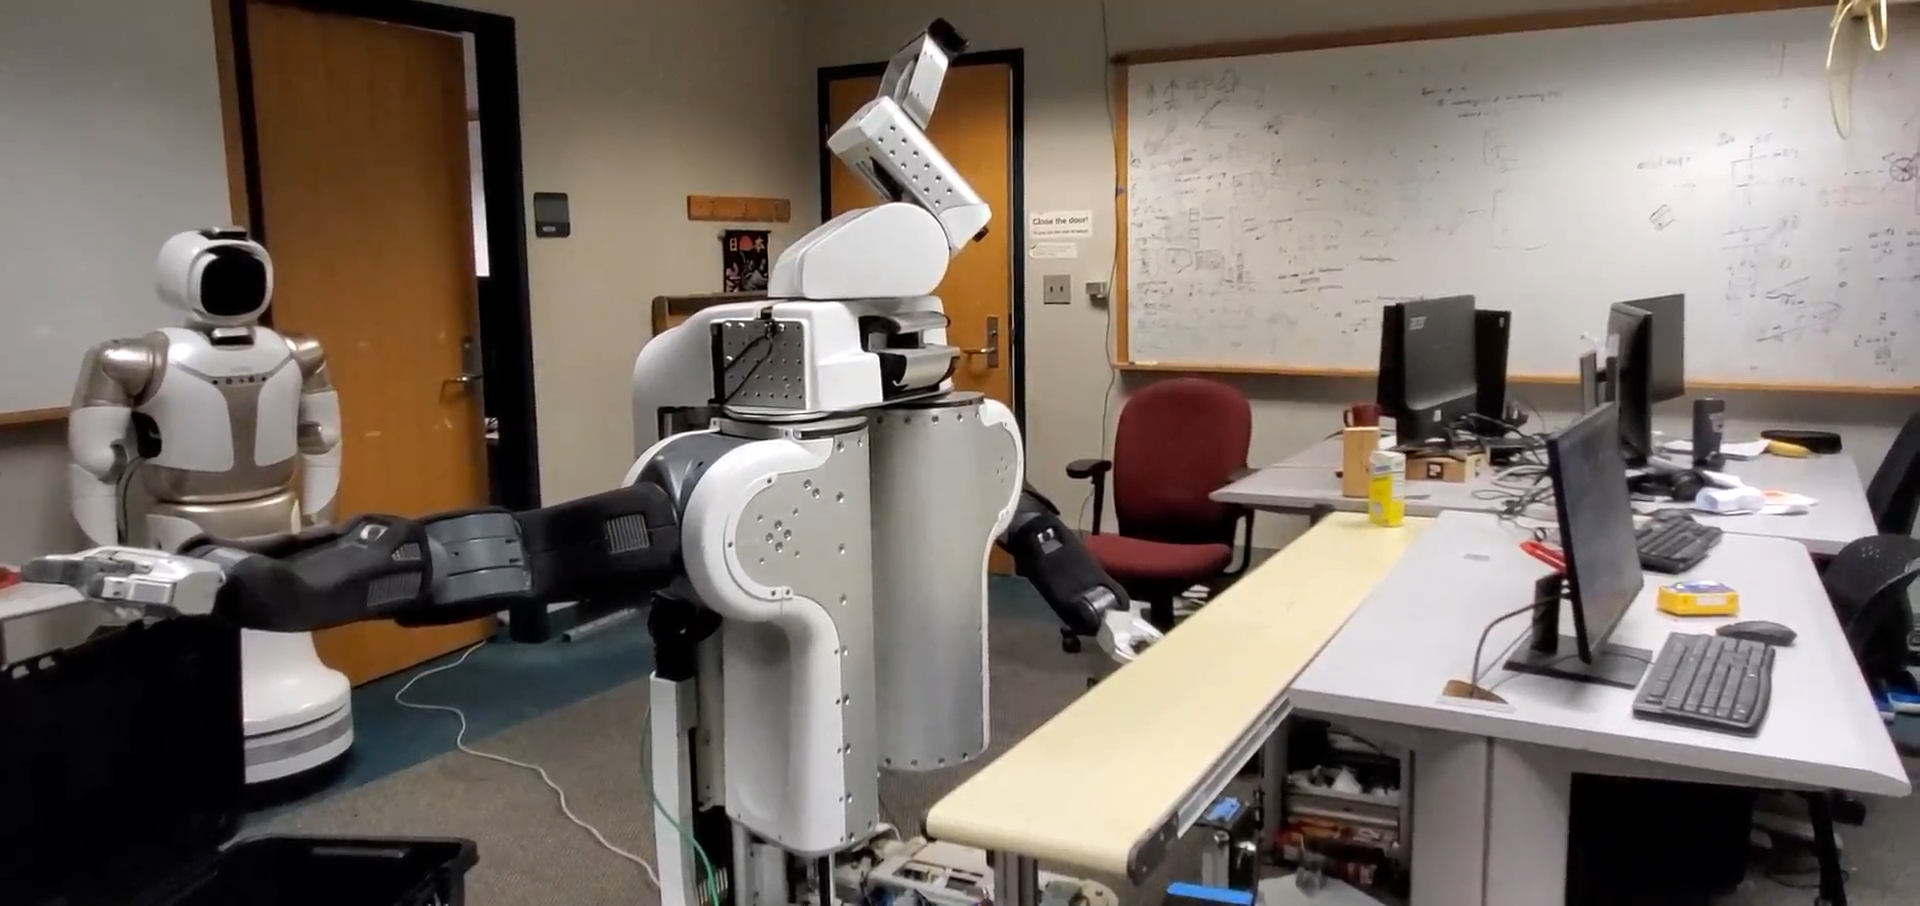
\includegraphics[trim=0 0 400 0, clip, width=\textwidth]{1}
        \caption{}
        \label{fig:demo1}
    \end{subfigure}
    \hspace{2mm}
    \begin{subfigure}{0.48\textwidth}
    %   \centering
        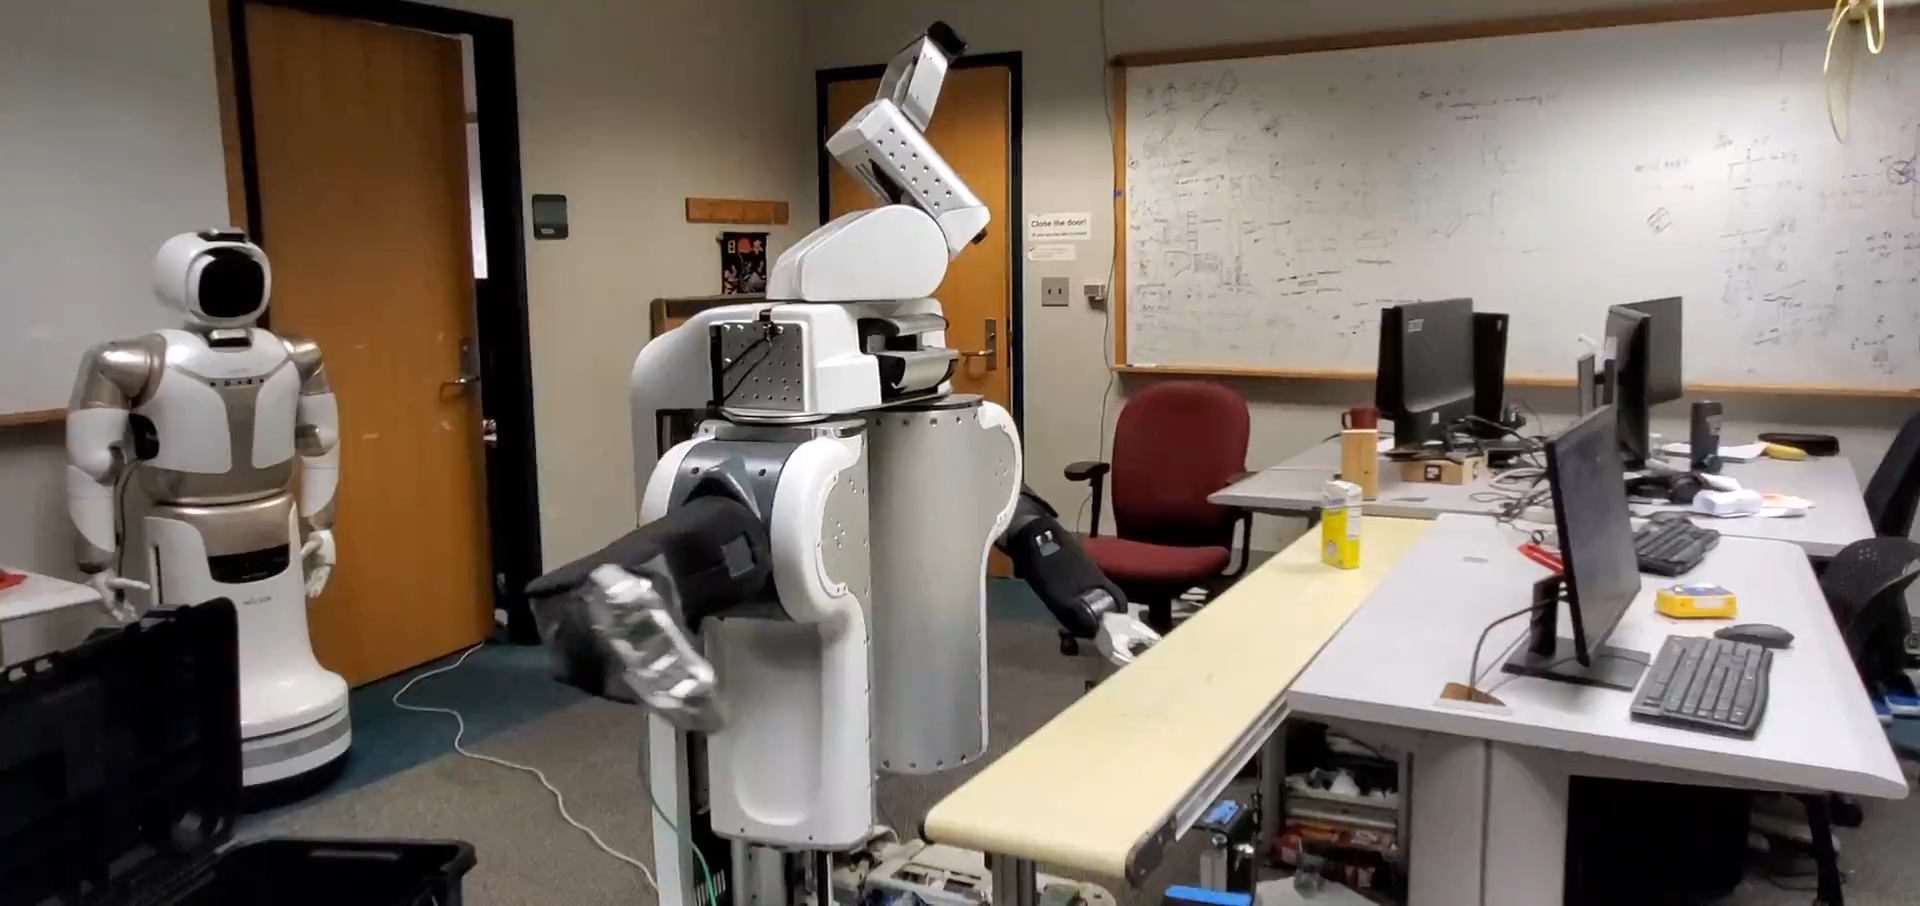
\includegraphics[trim=0 0 400 0, clip, width=\textwidth]{2}
        \caption{}
        \label{fig:demo2}
    \end{subfigure}
    \hspace{2mm}
    \begin{subfigure}{0.48\textwidth}
    %   \centering
        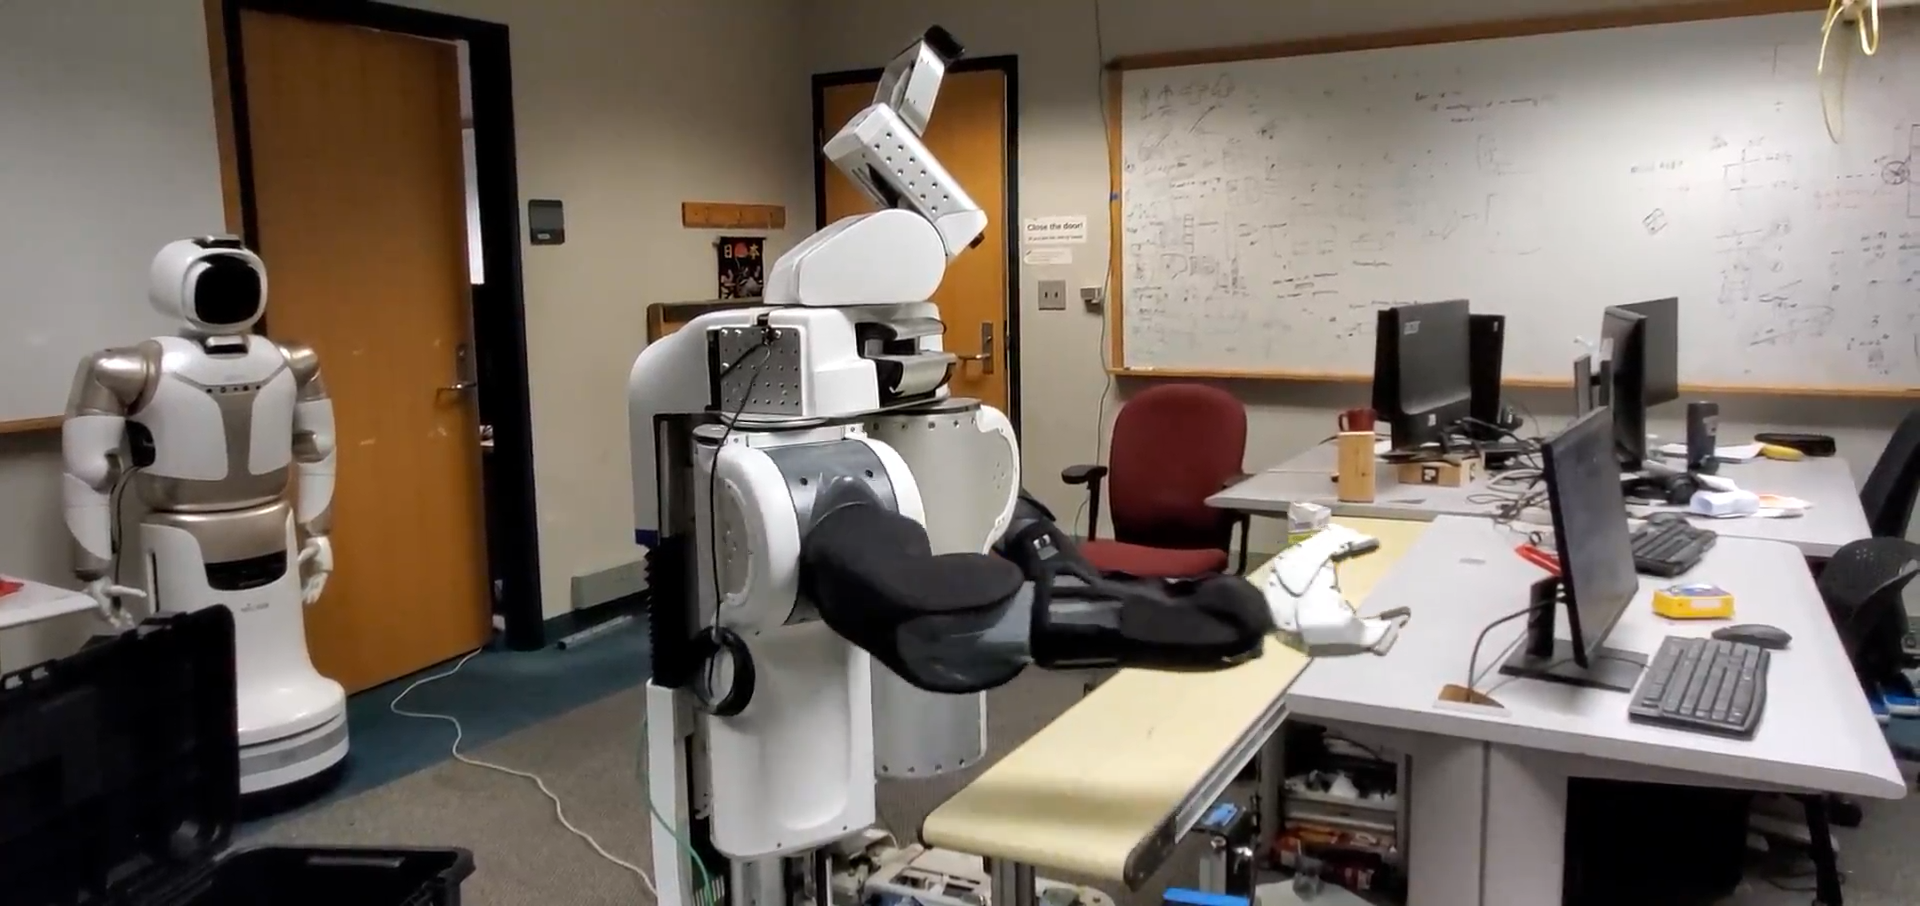
\includegraphics[trim=0 0 400 0, clip, width=\textwidth]{3}
        \caption{}
        \label{fig:demo3}
    \end{subfigure}
    \begin{subfigure}{0.48\textwidth}
    %   \centering
        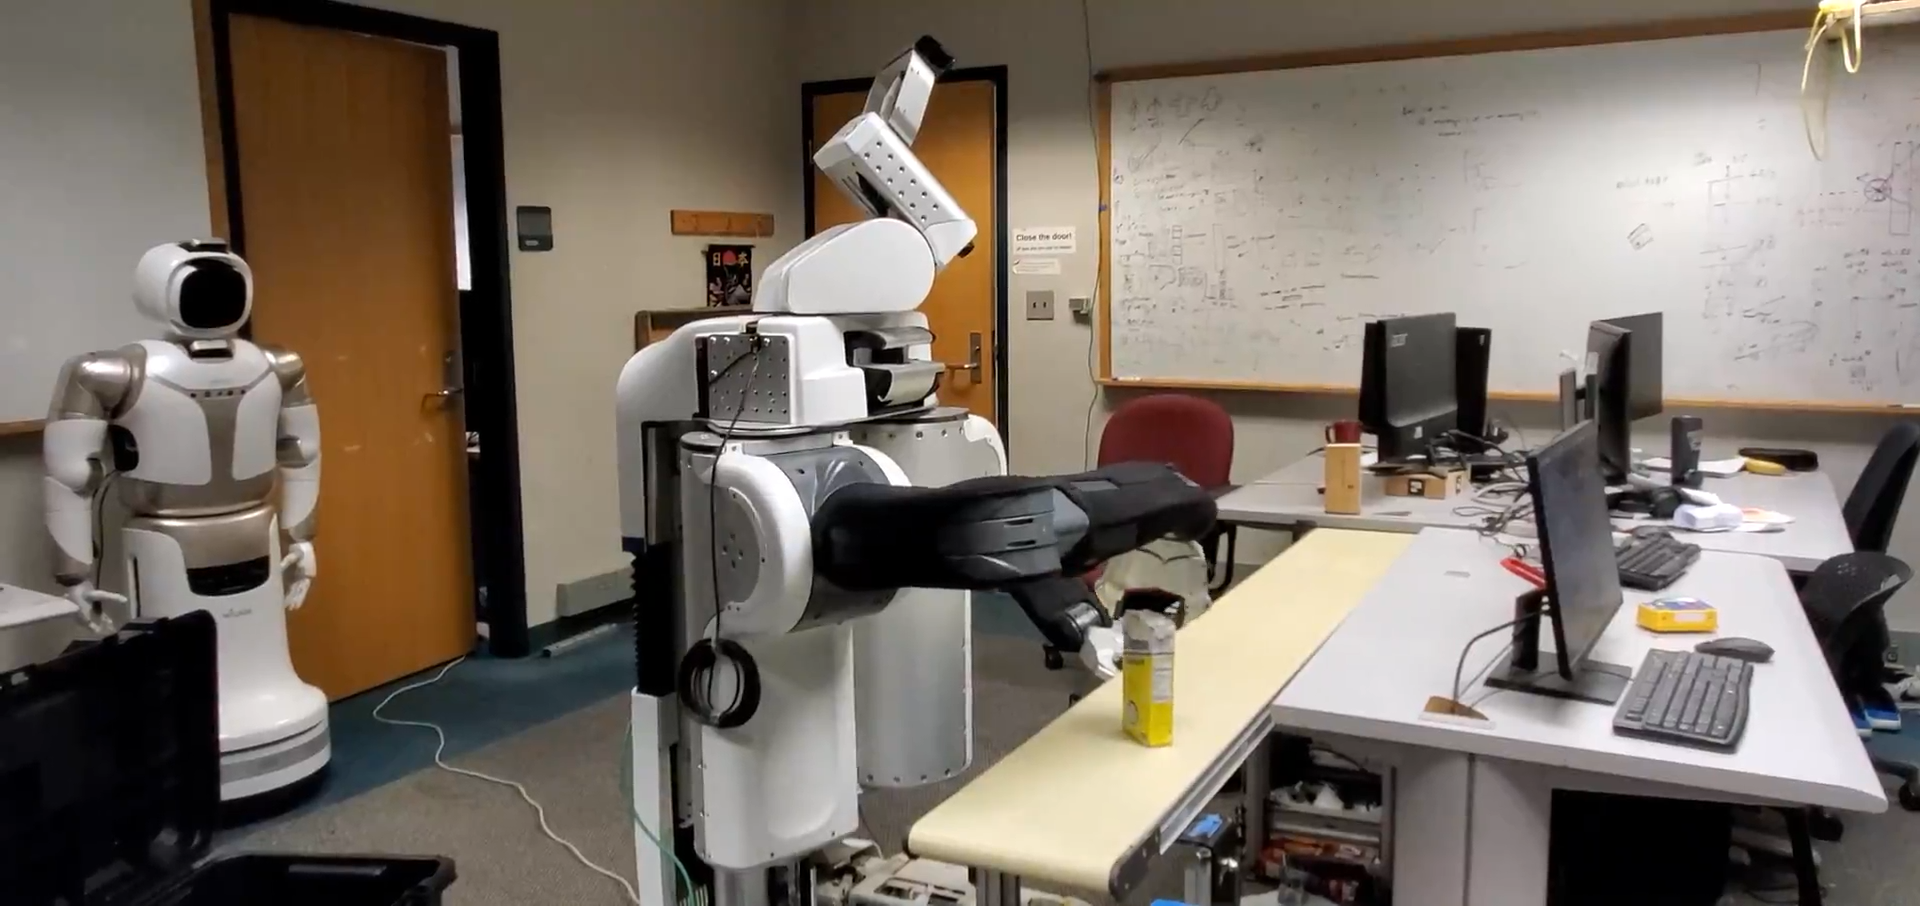
\includegraphics[trim=0 0 400 0, clip, width=\textwidth]{4}
        \caption{}
        \label{fig:demo4}
    \end{subfigure}
    \hspace{2mm}
    \begin{subfigure}{0.48\textwidth}
    %   \centering
        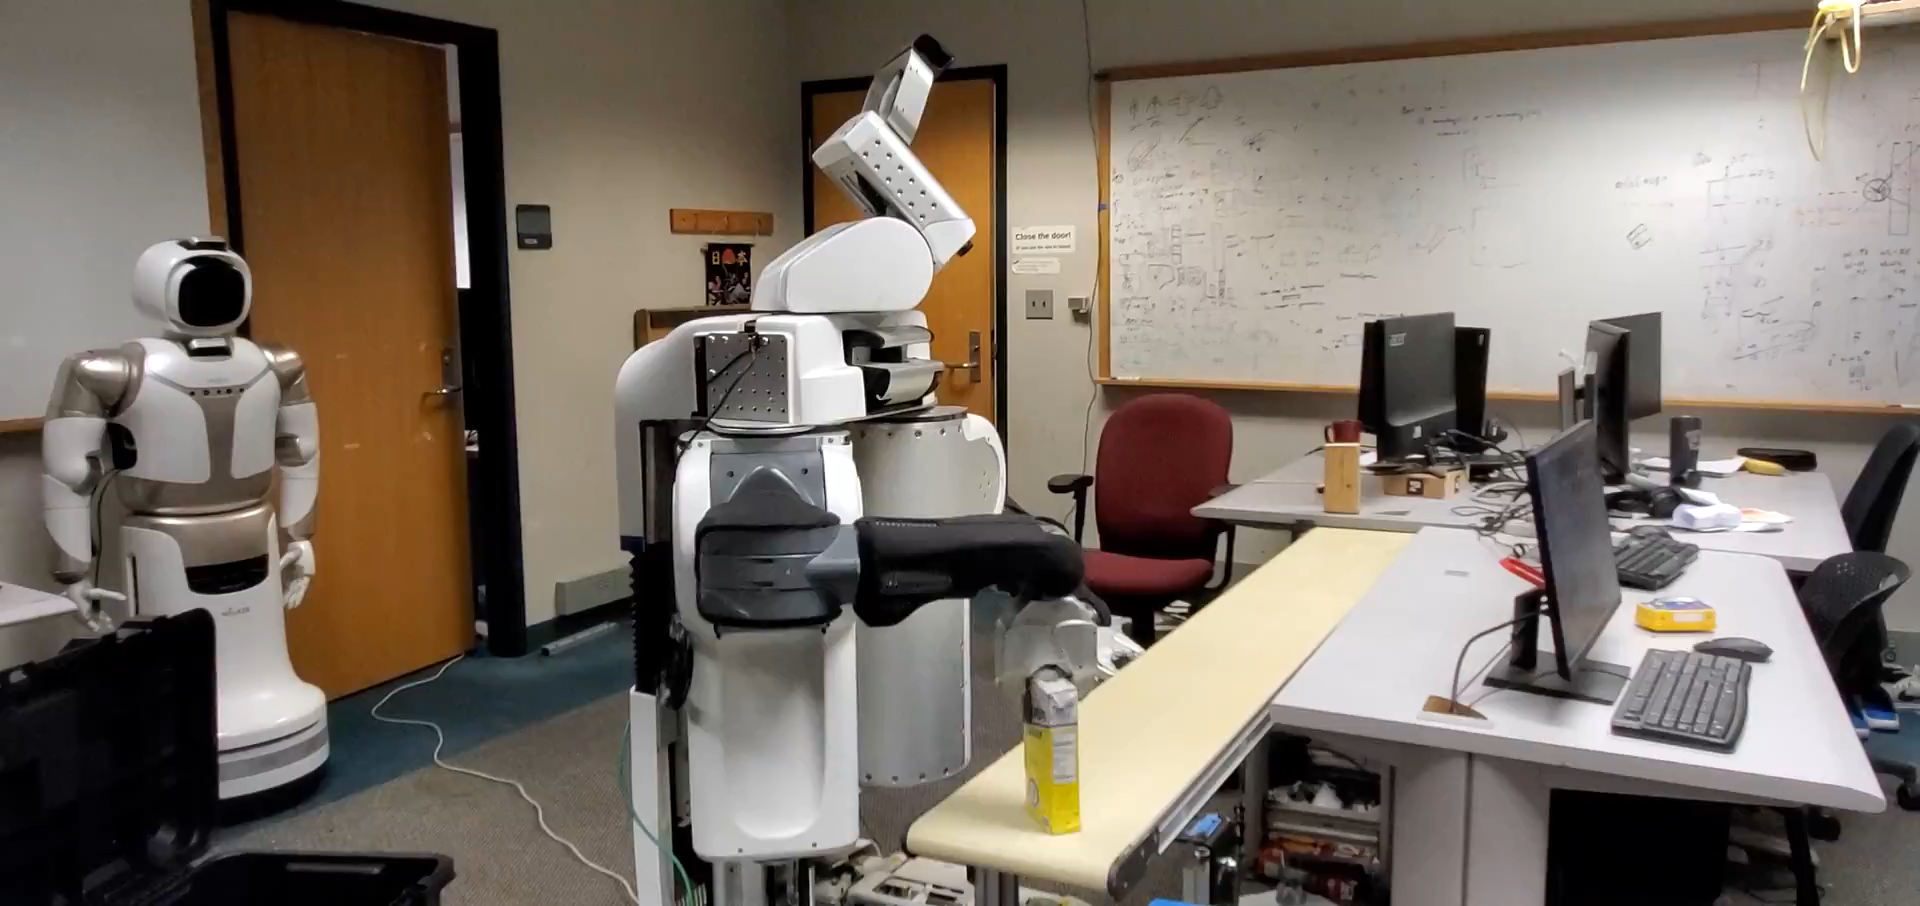
\includegraphics[trim=0 0 400 0, clip, width=\textwidth]{5}
        \caption{}
        \label{fig:demo5}
    \end{subfigure}
    \hspace{2mm}
    \begin{subfigure}{0.48\textwidth}
    %   \centering
        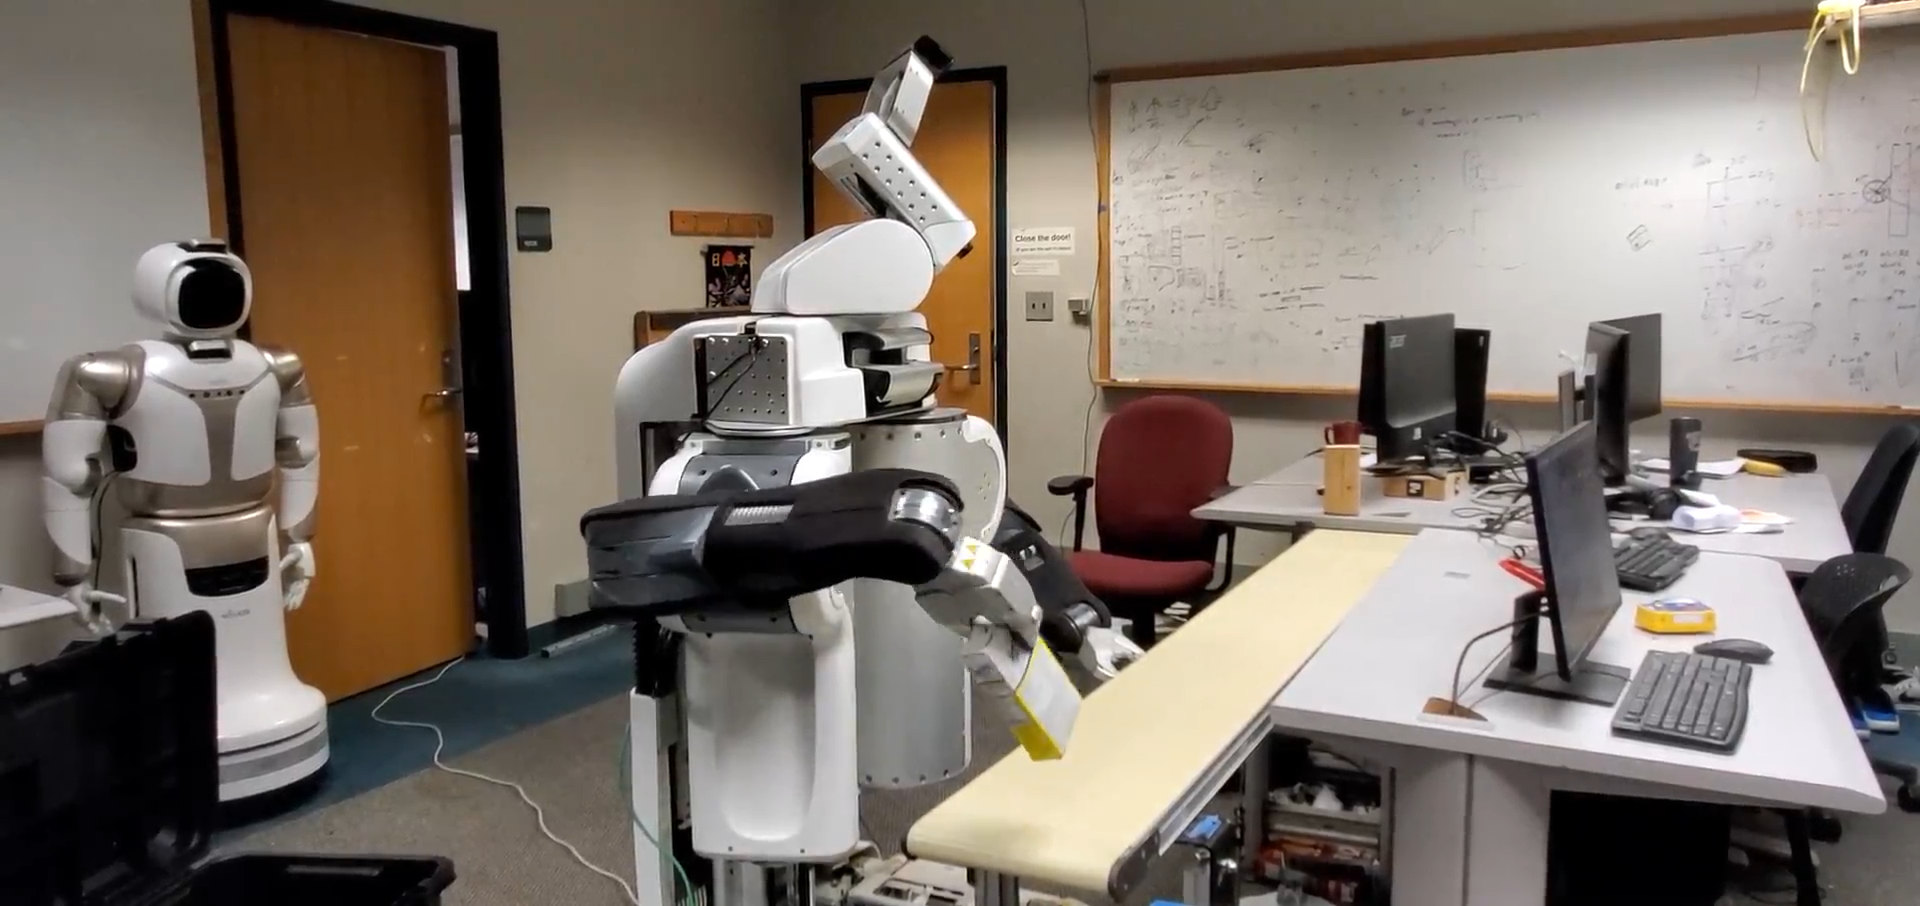
\includegraphics[trim=0 0 400 0, clip, width=\textwidth]{6}
        \caption{}
        \label{fig:demo6}
    \end{subfigure}
    \caption{\CaptionTextSize
    Snapshots from a real robot experiment.
    (\subref{fig:demo1})~The robot receives the first pose estimate from the perception system, generates the first plan within \Tbound and starts execution.
    %
    (\subref{fig:demo2})~The robot receives the second pose estimate with a pose correction of distance~3cm and replans to the new goal
    %
    (\subref{fig:demo3})~The robot receives the third and last pose estimate with no further correction and hence continues to follow the previous plan.
    (\subref{fig:demo4}) and (\subref{fig:demo5}) The robot executes the dynamic motion primitive to reach the grasp pose and glide along with the object.
    (\subref{fig:demo6}) The robot lifts up the sugar box from the conveyor.
    }
    \label{fig:demo}
\end{figure*}

\subsubsection{Simulation experiments}
We simulated the real world scenario to evaluate our method against other baselines. We compared our method with wA*~\cite{pohl1970heuristic}, E-graph~\cite{PCCL12} and RRT~\cite{lavalle1998rapidly}. 
For wA* and E-graph we use the same graph representation as our method. 
For E-graph we precompute five paths to randomly-selected  goals in \Gfull. 
We adapt the RRT algorithm to account for the under-defined goals. To do so, we sample pre-grasp poses along the conveyor 
%in the reachable workspace with a fine discretization 
and compute IK solutions for them to get a set of goal configurations for goal biasing. 
When a newly-added node falls within a threshold distance from the object, we use the same dynamic primitive that we use in the search-based methods to add the final grasping maneuver. If the primitive succeeds, we return success. We also allow wait actions at the pre-grasp locations.

For any planner to be used in our system, we need to endow it with a (possibly arbitrary) planning time bound to compute the future location of the object from which the new execution will start.
% (see Fig.~\ref{fig:tl}). 
%
If the planner fails to generate the plan within this time, the robot fails to react to that pose update and such cases are recorded as planning failure. 
%
We label a run as a pickup success if the planner successfully replans once after the object crosses the 1.0m mark. The mark is the mean of accurate perception range that was determined experimentally and used in the robot experiments as described in Section \ref{sec:robot_results}.
%
%
The key takeaway from our experiments (Table~\ref{tab:sim_results}) is that having a known time bound on the query time is vital to the success of the conveyor pickup task.

Our method shows the highest pickup success rate, planning success rate (success rate over all planning queries) and an order of magnitude lower planning times compared to the other methods. 
%
We tested the other methods with several different time bounds. After our approach E-graph performed decently well. RRT suffers from the fact that the goal is under-defined and sampling based planners typically require a goal bias in the configuration space. Another important highlight of the experiments is the number of planning cycles over the lifetime of an object. While the other approaches could replan at most twice, our method was able to replan thrice due to fast planning times.


\ignore{
\begin{table*}[t]
\centering
\begin{tabular}{|c||c||c|c|c||c|c|c||c|c|c|}
\hline
   & \textbf{Our Method} 
   & \multicolumn{3}{c|}{wA*}
   & \multicolumn{3}{c|}{E-Graph}
   & \multicolumn{3}{c|}{RRT}
   \\ \hline
   & $T_{b}$ = 0.2 
   & $T_{b}$ = 0.5 & $T_{b}$ = 1.0 & $T_{b}$ = 2.0 
   & $T_{b}$ = 0.5 & $T_{b}$ = 1.0 & $T_{b}$ = 2.0 
   & $T_{b}$ = 0.5 & $T_{b}$ = 1.0 & $T_{b}$ = 2.0 
   \\ \hline
Pickup success rate [\%]                   & 92.00     & 0.00      & 0.00     & 18.00      & 0.00        & 0.00       & 80.00       & 0.00       & 0.00       & 18.00      \\ \hline
Planning success rate [\%]                  & 94.67     & 4.00       & 17.00      & 19.00       & 31.00    & 80.00       & 90.00      & 12.00      & 9.00       & 13.00       \\ \hline
Planning time [s]                    & 0.0689       & 0.4329        & 0.6284        & 0.8241        & 0.2830        & 0.4194        & 0.3112        & 0.2718        & 0.2518        & 0.1966        \\ \hline
Planning episodes per pickup & 3            & 2             & 2             & 2             & 2             & 2             & 2             & 2             & 2             & 2             \\ \hline
Path cost [s]                         & 10.11        & 8.19          & 8.28          & 7.60          & 8.54          & 8.22          & 7.90          & 9.68          & 8.96          & 8.04          \\ \hline
%Expansions                        & 17.57        & 315.50        & 392.81        & 495.78        & 188.24        & 202.63        & 137.02        & 146.54        & 104.75        & 78.64         \\ \hline
\end{tabular}
\caption{Simulation results. Here $T_b$ denotes the (possibly arbitrary) time bound that the algorithm uses. Note that for our method $T_b = \Tbound$ is the time bound that the algorithm is ensured to compute a plan.}
\label{tab:sim_results}
\end{table*}
}

\subsubsection{Preprocessing}
The statistics of the preprocessing stage (i.e. running Alg.~\ref{alg:preprocess}) are shown in Table~\ref{table:pp}. The offline time bound $T_{\calP}$ used in all of our experiments was 10$s$
%
% took roughly 3.5 hours and the memory footprint following this stage was less than 20Mb.
%
% This supports our intuition that the domain allows for efficient compression of a massive amount of paths in a reasonable amount of preprocessing time.
%
In all experiments, we used $\Trc =$3.5$s$ and $\delta_t = $0.5$s$.
%
For the time-configuration planner the preprocessing took 2,534$s$. Only nine root paths are computed to cover 7,197 goals (three goals being unreachable and hence uncovered). For the states at $t=\Trc ($3.5$s)$, there were no latching failures and therefore, the algorithm terminates without preprocessing for earlier time stamps.
%
For the kinodynamic planner, the preprocessing takes about 7 hours. The dynamic constraints causes latching failures and therefore, the algorithm requires more preprocessing efforts. Due to latching failures at $t=$3.5, it needs to compute root paths for some of the states at this time step. Finally, it covers all the uncovered goals for states at $t=$3.0 via latching and finishes preprocessing.
% \begin{table}[t]
% % \centering
%     \resizebox{0.5\textwidth}{!}{ 
%         \begin{tabular}{ l | c c c c}
%           & \algname{wA*} & \algname{E-graph} & \algname{RRT} & \textbf{Our method} \\
%          \hline
%          Planning time [ms]& - (-) & - (-) & - (-) & \textbf{- (-)}\\
%          Success rate [$\%$]& - & - & - & \textbf{-}\\
%          No. of replans& - & - & - & \textbf{-}\\
%         \end{tabular}
%     }
%     \caption{Planning times, success rate and number of replanning queries averaged over 100 simulated runs of an object moving on the conveyor belt.}
%     \label{tab:stats_query}
% \end{table}

% ijrr
While we only performed experiments for a single target object with a single grasp, difference in object geometries and grasps may affect the performance of the planner. Specifically, the number of reachable goals for any given $\Sstart$ would change depending on the difficulty of the motion planning problems that the CTMP algorithm attempts to solve. This would impact the query success rate as well as the preprocessing time of the CTMP algorithm.

\newpage
\chapter{CTMP for Semi-static Environments}
\label{sec:icra}
\section{Overview}
%% motivate the need of planners for semi-static environments
In a wide range of environments, be it warehouses, factories or homes, robots share their workspace with humans or other robots. While the obstacle occupancy in such environments is largely fixed or static, yet small regions within these environments may vary in occupancy during operation. We categorise such environments as \emph{semi-structured}. Additionally in these applications robots are often performing repetitive tasks and require fast and reliable motion planning capabilities.

%% use example
Consider the scenario in Fig.~\ref{fig:cover}. The robot must grasp the bowl while avoiding the pitchers, table and walls.
%Most of the environment (e.g. table, walls, free space above the table etc.) can be assumed to be known, and since the task of picking up an object from a tabletop is repetitive, some information from previous similar planning queries can be re-used to speedup planning.
Most of the environment (e.g. table, walls, free space above the table etc.) can be assumed to be known, and since the task is repetitive some information from previous planning queries can be re-used to speedup planning.
 %More commonly used planning algorithms such as RRTs neither exploit the distinction between static and movable obstacles, nor do they take advantage of the repetitive nature of planning problems to speedup planning. 
Commonly used algorithms such as RRTs~\cite{kuffner2000rrt} neither exploit the distinction between static and movable obstacles nor take advantage of the repetitive nature of planning problems to speedup planning. 

%% existing approaches
%Preprocessing based methods like PRMs, precompute roadmaps to speedup online planning. They
Roadmap-based methods like PRMs are either limited to fully static environments or incur considerable overheads in repair operations which they require to handle movable obstacles. While there exists several algorithms that use information from previous similar planning episodes such as Lightning~\cite{berenson2012robot}, E-graphs~\cite{Phillips-RSS-12} etc., their performance also degrades when the past information is invalidated by the changes in the environment. All these methods therefore can not provide fixed-time planning guarantees. 

%% my prior work
Recently, provably fixed-time motion planning approaches have been proposed for repetitive tasks in fully known environments~\cite{islam2019provable},~\cite{islam2020provably}. They precompute library of paths using the known models of obstacles and other task-specific information. These approaches have been used before for mail-sorting~\cite{islam2019provable} and for grasping objects moving down a conveyor belt~\cite{islam2020provably}. They, however, are also not designed to handle movable obstacles.

\begin{figure}[bt]
\centering
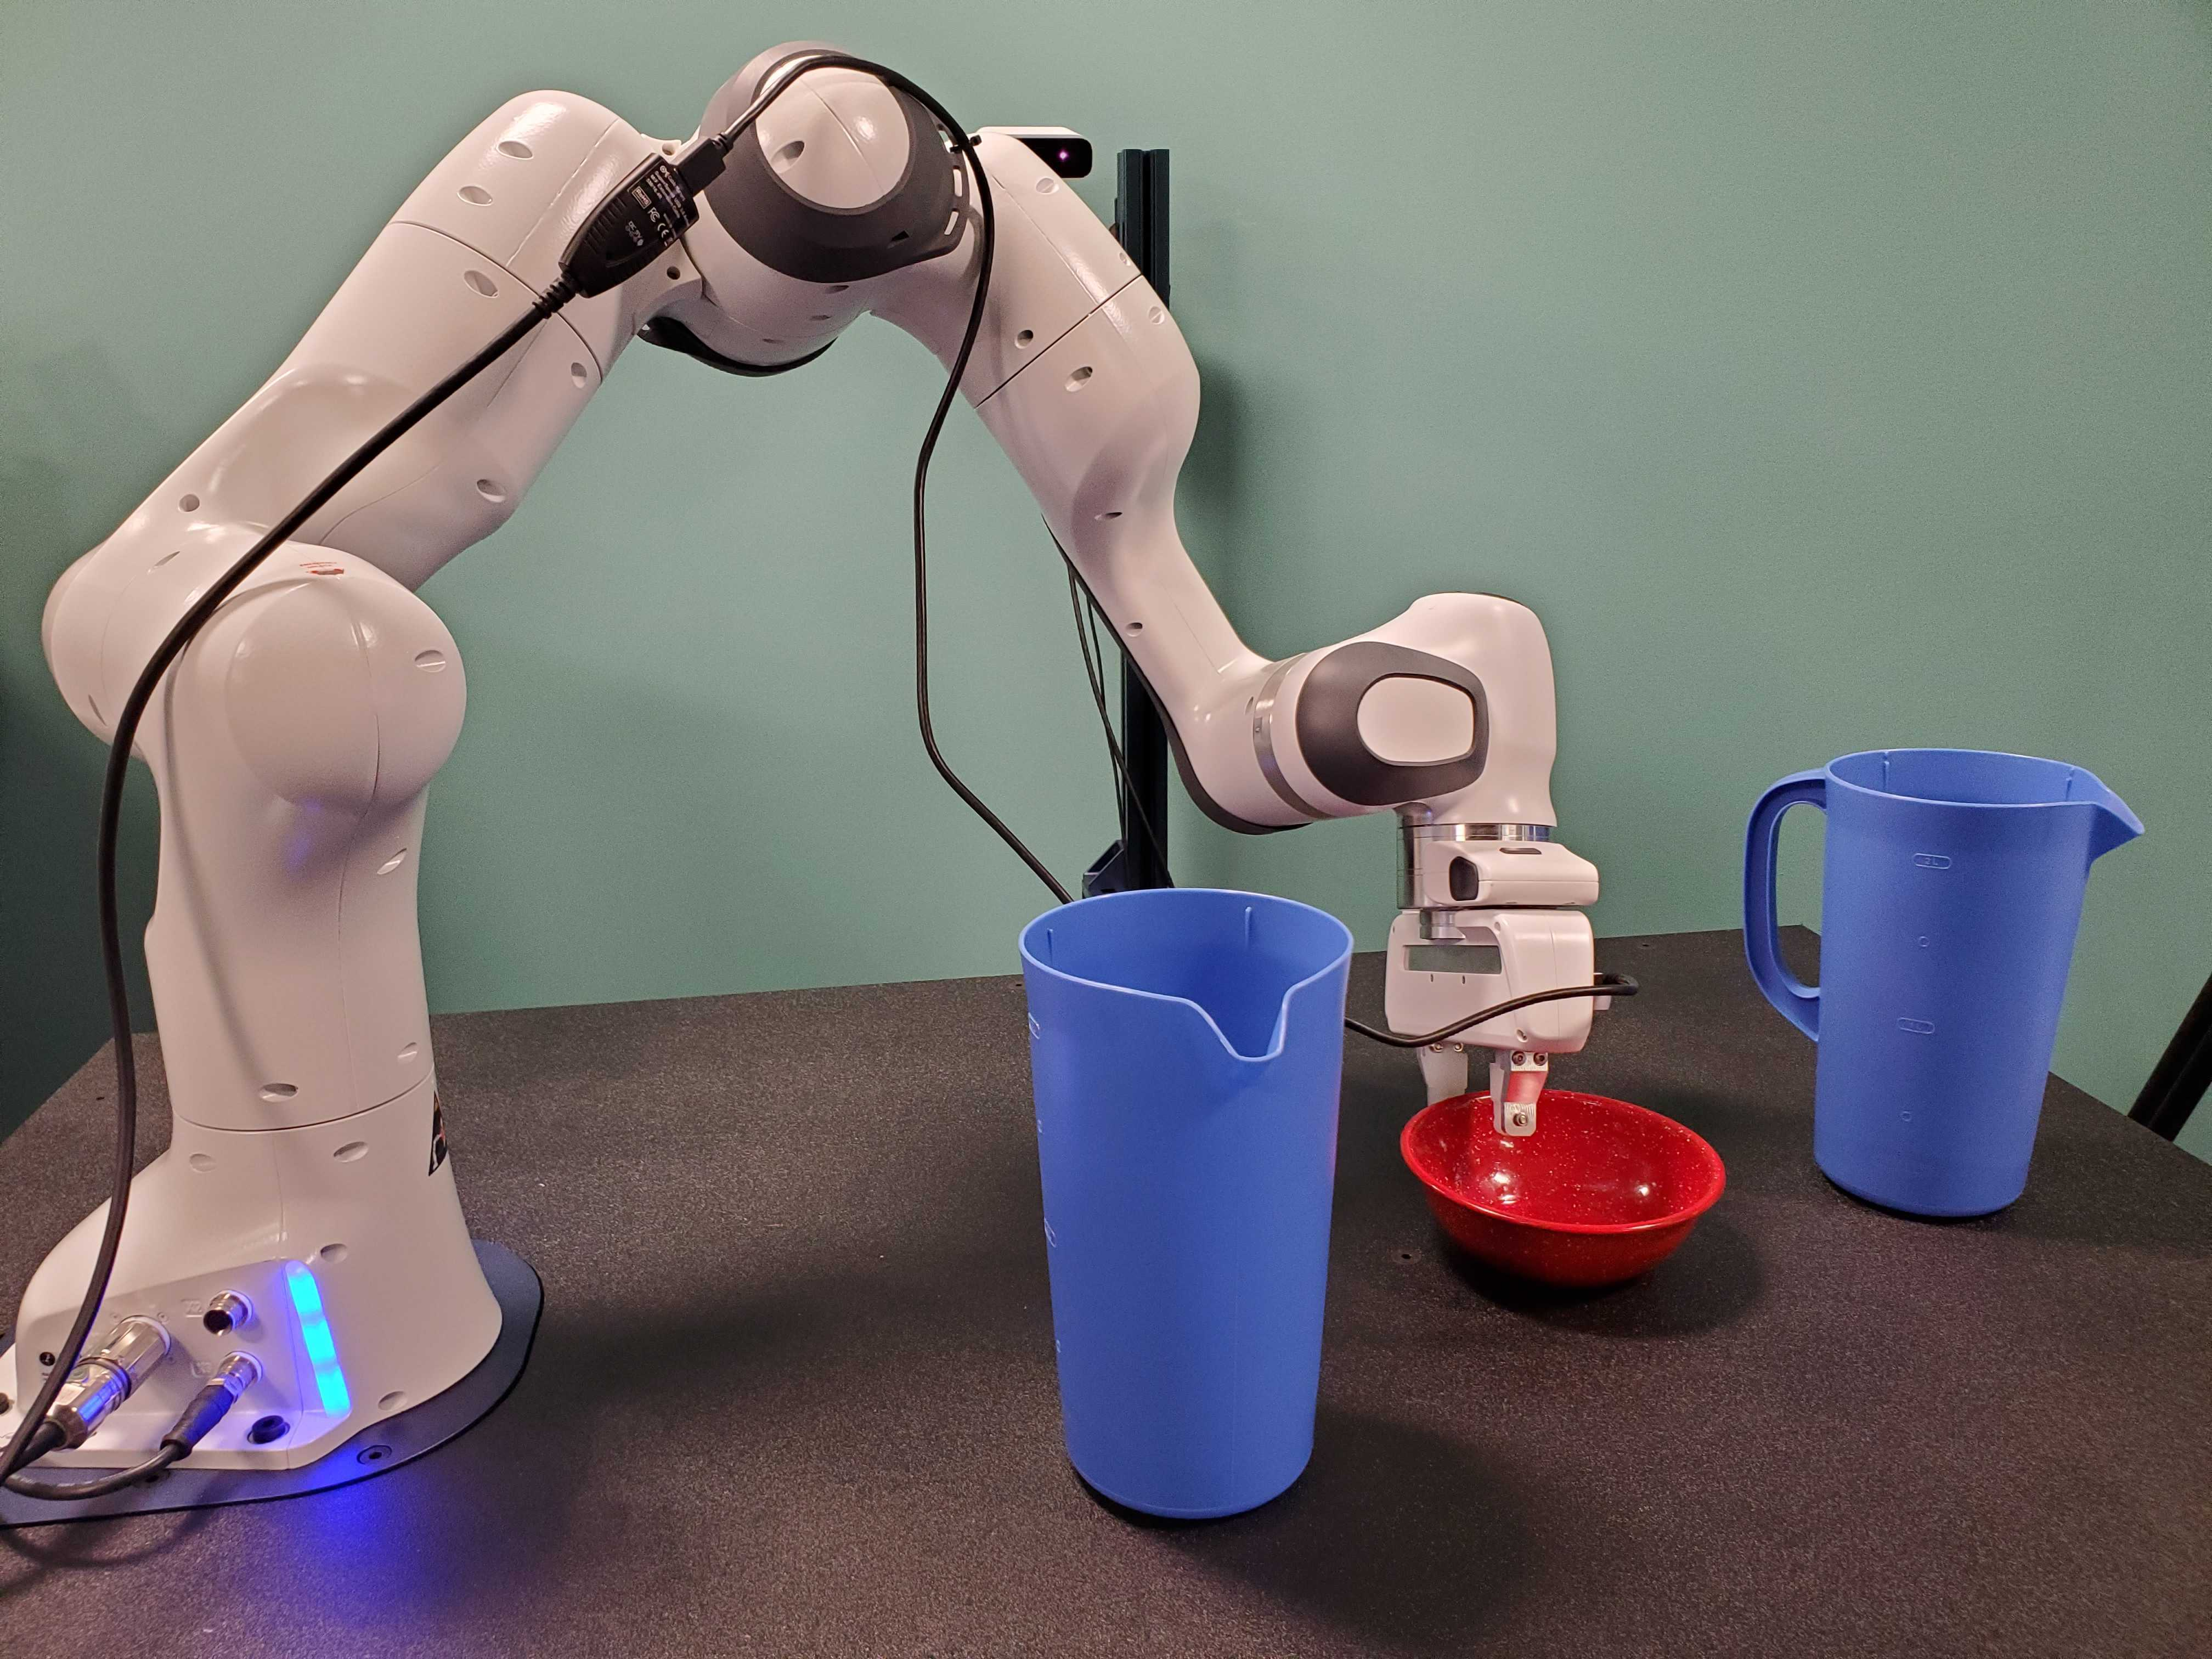
\includegraphics[width=\columnwidth]{figs/cover.jpg}
\caption{Semi-structured tabletop manipulation scenario --- The robot must grasp the bowl while avoiding pitchers and the table itself; the pitchers and bowl may be at any position. The Alternate Paths Planner (APP) guarantees to find solution for any configuration within few microseconds.}
\label{fig:cover}
\vskip -0.5cm
\end{figure}

%% our contribution
%In this work we aim to extend these recent approaches to be able to handle movable obstacles while still provably fixed-time planning guarantees.
In this work we extend these approaches to handle movable obstacles while still guaranteeing provably fixed-time planning.
%key idea of our approach is to generate multiple alternative paths for each planning problem, such that for any configuration of movable obstacles, one of these alternative paths is guaranteed to be traversable.
The key idea is to generate multiple alternative paths for each planning problem, such that for any configuration of movable obstacles, one path is guaranteed to be traversable.
One approach to achieve this is to enforce %a constraint
that these paths are \emph{disjoint}: they are separated enough that no single obstacle configuration can intersect two paths simultaneously.
To get the aforementioned guarantee, $n$ movable obstacles require generating only $n+1$ fully disjoint paths.
%However, if $n+1$ disjoint paths cannot be found for the given problem, our approach uses more preprocessing and finds additional paths to provide the guarantee.
However, if $n+1$ disjoint paths cannot be found for the given problem, we find additional additional paths partially-overlapping paths to provide the same guarantee.
%We make some simplistic assumptions about the geometry of movable obstacles to provide strong guarantees on the planning time.
We call this approach \emph{Alternative Paths Planner (APP)}

%APP can be applied to many performance critical real-world robotics use cases such as mail-sorting, conveyor-belt picking, and shelving. 
APP can be applied to performance-critical real-world use cases such as mail-sorting, conveyor-belt picking, and shelving. 
For scenarios with multiple movable obstacles, we demonstrate microsecond-scale lookup times and achieve a 100\% success rate. We include experimental results from three domains, compare with state-of-the-art existing approaches and validate our approach with a real-world case study. 

\section{Algorithmic Framework}
%\subsection{Problem Setup and Assumptions}
\label{subsec:setup}
%Let \calX be the configuration space of the robot. Let $\Sstart \in \calX$ be a fixed start configuration of the robot and \calG be the goal region. 
Let \calX be the configuration space of the robot, $\Sstart \in \calX$ be a fixed start configuration of the robot, and \calG be the goal region. 
%\calG could be defined in the configuration space \calX i.e $\calG \subset \calX$ 
\calG could be defined in the configuration space \calX (i.e $\calG \subset \calX$) or it could be under-defined, e.g., as the position in $\mathbb{R}^3$ or pose in $SE(3)$ of a target object or the robot end-effector. \calG is discretized to have a finite set of goals $G$. 

Let \calW be a 3D semi-static world in which the robot operates. \calW contains a fixed set of movable obstacles $\calO = \{o_1, o_2, o_3,...,o_n\}$, that occupy $\calW_\calO \subset \calW$, and can be displaced in between different planning queries. A movable obstacle $o_i$ can attain any configuration within a space $\calQ(o_i)$ which is discretized into a set of configurations $Q(o_i)$. Additionally, \calW has a partial occupancy $\calW_S$, which is static i.e $\calW_S = \calW \backslash \calW_\calO$. The motion planning problem is to find a collision-free path for the robot operating in \calW from \Sstart to any goal $g \in G$.

% \begin{assumption}
% \label{assum:1}
% We assume that all obstacles $o_i \in \calO$ are identical in geometry.
% \end{assumption}

\subsection{Approach}
%In this work, we aim to develop an algorithm that can provide provable bounds on the planning time for each planning query.
In this work, we describe an algorithm that provides provable bounds on the planning time for each planning query, where these bounds are small enough to guarantee real-time performance.
%Furthermore we want the bounds to be small to guarantee real-time performance.
%Before we describe our approach, we begin by briefly describing a strawman algorithm which solves the aforementioned problem with the provable bounded-time guarantee but is practically prohibitive due to its memory and computational requirements.
We begin by briefly describing a strawman algorithm which solves the aforementioned problem with the provable bounded-time guarantee but is practically prohibitive due to its memory and computational requirements.
%This will also prepare the ground to describe our method which also provides bounded-time guarantee but with minimal memory and computational load.


\subsubsection{Strawman Algorithm}
Assume that we have access to a motion planner \calP that can be used offline to find feasible paths for the given planning problems. The naive approach
%of providing bounded-time guarantee
is to precompute and store paths for all possible planning problems using \calP %owing to the problem setup described in Sec.~\ref{subsec:setup},
offline in a preprocessing stage.
%, and at 
%Then, at query time a lookup table is used to answer any query in bounded time. Specifically, it requires computing the lookup table
At query time, a lookup table can answer any query in bounded time. Specifically, we precompute the lookup table
$$
\calM : G \times Q(o_1) \times Q(o_2) \times ... \times Q(o_n) \rightarrow \{\pi_1, \pi_2,\pi_3,...\}
$$

\noindent that maps every configuration of goal and the $n$ obstacles to a unique path $\pi_i$ resulting in $|G|.|Q(o_1)|.|Q(o_2)|....|Q(o_n)|$ paths. Assuming that each object $o_i$ can be in the same set of configurations in $\calW$, the space complexity then is $O(|G|.|Q(o_i)|^{n})$ which is exponential in the number of movable objects in \calO.
%This complexity clearly is severely restrictive in practice.

\subsubsection{Proposed Approach}
While the strawman algorithm provides bounded-time guarantees, its memory and precomputation load is prohibitive for practical purposes. To this end we propose an algorithm that can provide bounded-time guarantees but requires significantly smaller resources in practice.

Our key idea is that, for the given \Sstart and $g$, instead of precomputing path for every possible configuration of obstacles \calO, our algorithm systematically precomputes a small set of paths $\Pi_g$ from \Sstart to $g$ with the guarantee that for any possible configuration of \calO in \calW, at least one path $\pi \in \Pi_g$ will be collision free. At query time, this path can be looked up efficiently in provably bounded time.

\subsection{Algorithm Overview}
Before we describe the approach, we introduce some terminology.

\begin{definition}[Envelope]
\label{def:envp}
For a path $\pi$, an envelope is a set of all obstacle configurations $e_\pi \subset Q(o_1) \cup Q(o_2) \cup...\cup Q(o_n)$, that collide with any robot state $s \in \pi$, except \Sstart, and are not within $\epsilon$ distance of $\textsc{Proj}(g)$
\end{definition}

\noindent where $\textsc{Proj}(g)$ is the projection of $g$ in $\mathbb{R}^3$ and $\epsilon$ is in Euclidean space. Fig.~\ref{fig:envp} illustrates an envelope with a simple example.
The implementation details of envelope construction for the manipulation domain are discussed in Sec.~\ref{sec:impl_details}

\begin{figure}[bt]
\centering
% \includegraphics[width=\columnwidth]{figs/envp.pdf}
\includegraphics[width=\columnwidth]{figs/envp_grid.pdf}
\caption{Depiction of an envelope for a single movable obstacle $o$: the blue rectangles represent the robot states in $SE(2)$ along the path $\pi$, the red circle is the movable obstacle $o$ that can have any position in $Q(o) \in \mathbb{R}^2$ and the small circles show positions $q(o)$ for which $o$ collides with $\pi$ and thus constitute the envelope $e_\pi$}
\label{fig:envp}
% \vskip -0.5cm
\end{figure}

\begin{definition}[Disjoint paths]
\label{def:disjointness}
The paths $\pi_1,\pi_2,...,\pi_n$ are disjoint if their corresponding envelopes $e_{\pi_1},e_{\pi_2},...e_{\pi_n}$ are disjoint sets.
\end{definition}

%For simplicity, consider a simple planning problem of finding a collision-free path from \Sstart to a goal $g \in G$ in the presence of a single movable obstacle $o$ and some static occupancy $\calW_S$.
Consider finding a collision-free path from \Sstart to a goal $g \in G$ in the presence of a single movable obstacle $o$ and some static occupancy $\calW_S$.
We first find a path $\pi_1$ from \Sstart to $g$ using \calP while avoiding collisions with only $\calW_S$.
Next we construct an envelope $e_{\pi_1}$ around $\pi_1$, where $e_{\pi_1}$ (by Def.~\ref{def:envp}) is the set of all configurations that $o$ can take that invalidate $\pi_1$.
If $e_{\pi_1}$ is non-empty, we attempt to find a second path $\pi_2$ that avoids collisions with $\calW_S$ as well as with the occupancy of $e_{\pi_1}$.
%This gives us two disjoint paths $\pi_1$ and $\pi_2$ (since $e_{\pi_2}$ and $e_{\pi_1}$ would be disjoint by Def.~\ref{def:disjointness}).
This gives us two disjoint paths $\pi_1$ and $\pi_2$, by Def.~\ref{def:disjointness}.
%These two paths constitute the minimal set of paths with the guarantee that for any configuration $q(o) \in Q(o)$, one of these two paths will be collision free.
These two paths constitute the minimal set of paths with the guarantee that for any configuration $q(o) \in Q(o)$, one path will be collision free.
%At query time given any configuration $q(o)$, we can check if it lies within $e_{\pi_1}$ or not and based on that, use the path $\pi_2$ or $\pi_1$ respectively. By storing envelopes as sets implemented using hash tables, we can check it in constant time~\cite{czech1997perfect}.
At query time given any configuration $q(o)$, we can check if it lies within $e_{\pi_1}$ or not and use the path $\pi_2$ or $\pi_1$ respectively. By storing envelopes as sets implemented using hash tables, we can check it in constant time~\cite{czech1997perfect}. Note that if $e_{\pi_1}$ is empty, we only require a single path $\pi_1$.

\textbf{Extending to $n$ movable obstacles:} A single movable obstacle, requires at most two disjoint paths. Extending to $n$ objects would require at most $n+1$ disjoint paths. Therefore, for the scenarios in which the required number of disjoint paths exists and \calP can find them within a given allowed planning time, the computational complexity of the preprocessing phase grows linearly with number of movable obstacles i.e $O(|\calO|)$.
If \calP fails to find the required number of disjoint paths, however,
%which is possible if the paths do not exist or \calP cannot find them in a finite preprocessing time,
then this method is incomplete as is, and it would require more preprocessing efforts to find more paths to satisfy the criterion that for any possible configuration of the set of obstacles \calO, at least one of the paths from the set is guaranteed to be collision free. %The following section discusses the details of the complete preprocessing and query algorithms.

\subsection{Algorithm Details}
%We now describe the two phases of our algorithm, i.e., the preprocessing and the query phases.
We now describe the two phases of our algorithm: the preprocessing and the query phases.

\subsubsection{Preprocessing}
The preprocessing algorithm is described in Alg.~\ref{alg1} and is illustrated in Fig.~\ref{fig:illustration}. It starts with finding the first collision-free path $\pi_1$ from \Sstart to the given goal $g \in G$ in $\calW_S$. For each computed path $\pi_j$, the algorithm maintains the set of envelopes $\calE_{\pi_j}$ that were avoided while computing $\pi_j$. For the first path $\pi_1$, the set $\calE_{\pi_1}$ is empty since \calP only considers $\calW_S$ for this step. The algorithm then runs a loop for $n=|\calO|$ iterations, attempting to find $n$ more mutually disjoint paths (loop at line~\ref{alg1:l1}). Another loop at line~\ref{alg1:l2} is needed for the case when $n+1$ disjoint paths do not exist and therefore, more than one paths are computed in a single iteration of loop at line~\ref{alg1:l1}.
In every iteration of the loop at line~\ref{alg1:l2}, the algorithm first constructs the envelope $e_{\pi_j}$ around the path $\pi_j$ found in the previous iteration of loop at line~\ref{alg1:l1}. Next, $\pi_j'$ is computed while avoiding collisions with the occupancy of the set of envelopes $\calE_{\pi_j}'$, which is the union of $e_{\pi_j}$ and the envelopes in $\calE_{\pi_j}$. $\calE_{\pi_j}'$ thus constitutes the set of avoided envelopes for $\pi_j'.$

For the case when \calP fails to find the disjoint path at any iteration of loop at line~\ref{alg1:l1}, the algorithm bisects one of the envelopes (line~\ref{alg1:bisect} and Alg.~\ref{alg2}) that \calP attempted to avoid, resulting in two sets of envelopes (each one containing a bisected envelope along with the remaining envelopes). \calP then tries to find paths around the occupancy of envelopes in each of the two sets independently. Note that this process (Alg.~\ref{alg2}) repeats recursively until either \calP successfully finds paths around all the newly created sets of envelopes or until further recursion is not possible. The latter occurs in the worst case, when the algorithm recurses down to the deepest level, where each envelope contains individual obstacle configurations. Owing to the structure of these envelopes, we implement them as binary-trees. Because of this envelope bisection, the algorithm may compute more than one path in a single iteration of loop at line~\ref{alg1:l1}. It therefore maintains a set of paths $\Pi_i$ for each iteration and attempts to compute disjoint paths for all paths $\pi_j \in \Pi_i$ in the following iteration.

The preprocessing algorithm (Alg.~\ref{alg1}) returns a database of paths $\Pi_g = \Pi_1 \cup \Pi_2 \cup ... \cup \Pi_{n+1}$ from \Sstart to a goal $g$ with the guarantee that for any possible configuration of obstacles \calO, one of the paths $\pi \in \Pi_g$ is collision free. To cover the full goal region $G$, Alg~\ref{alg1} is called for each $g \in G$ in the preprocessing phase.

\begin{figure*}[t]
    \centering
    \begin{subfigure}{0.48\textwidth}
    %   \centering
        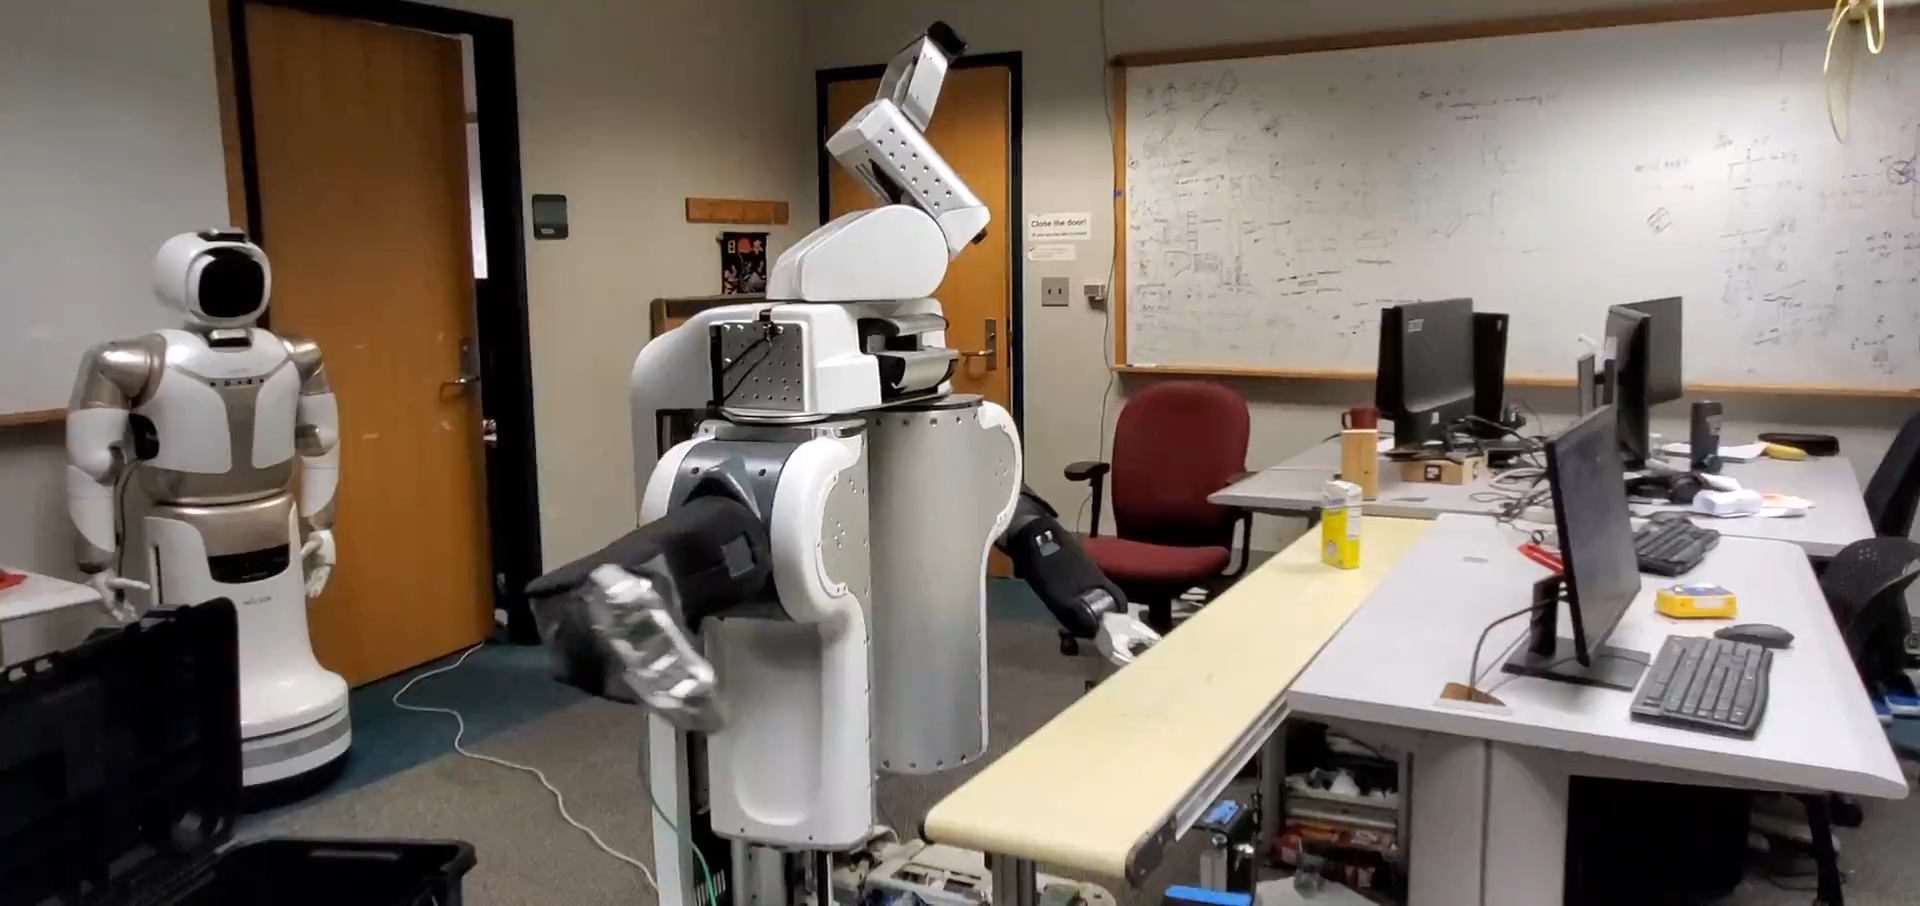
\includegraphics[width=\textwidth]{2.pdf}
        \caption{}
        \label{fig:p1}
    \end{subfigure} 
    \begin{subfigure}{0.48\textwidth}
    %   \centering
        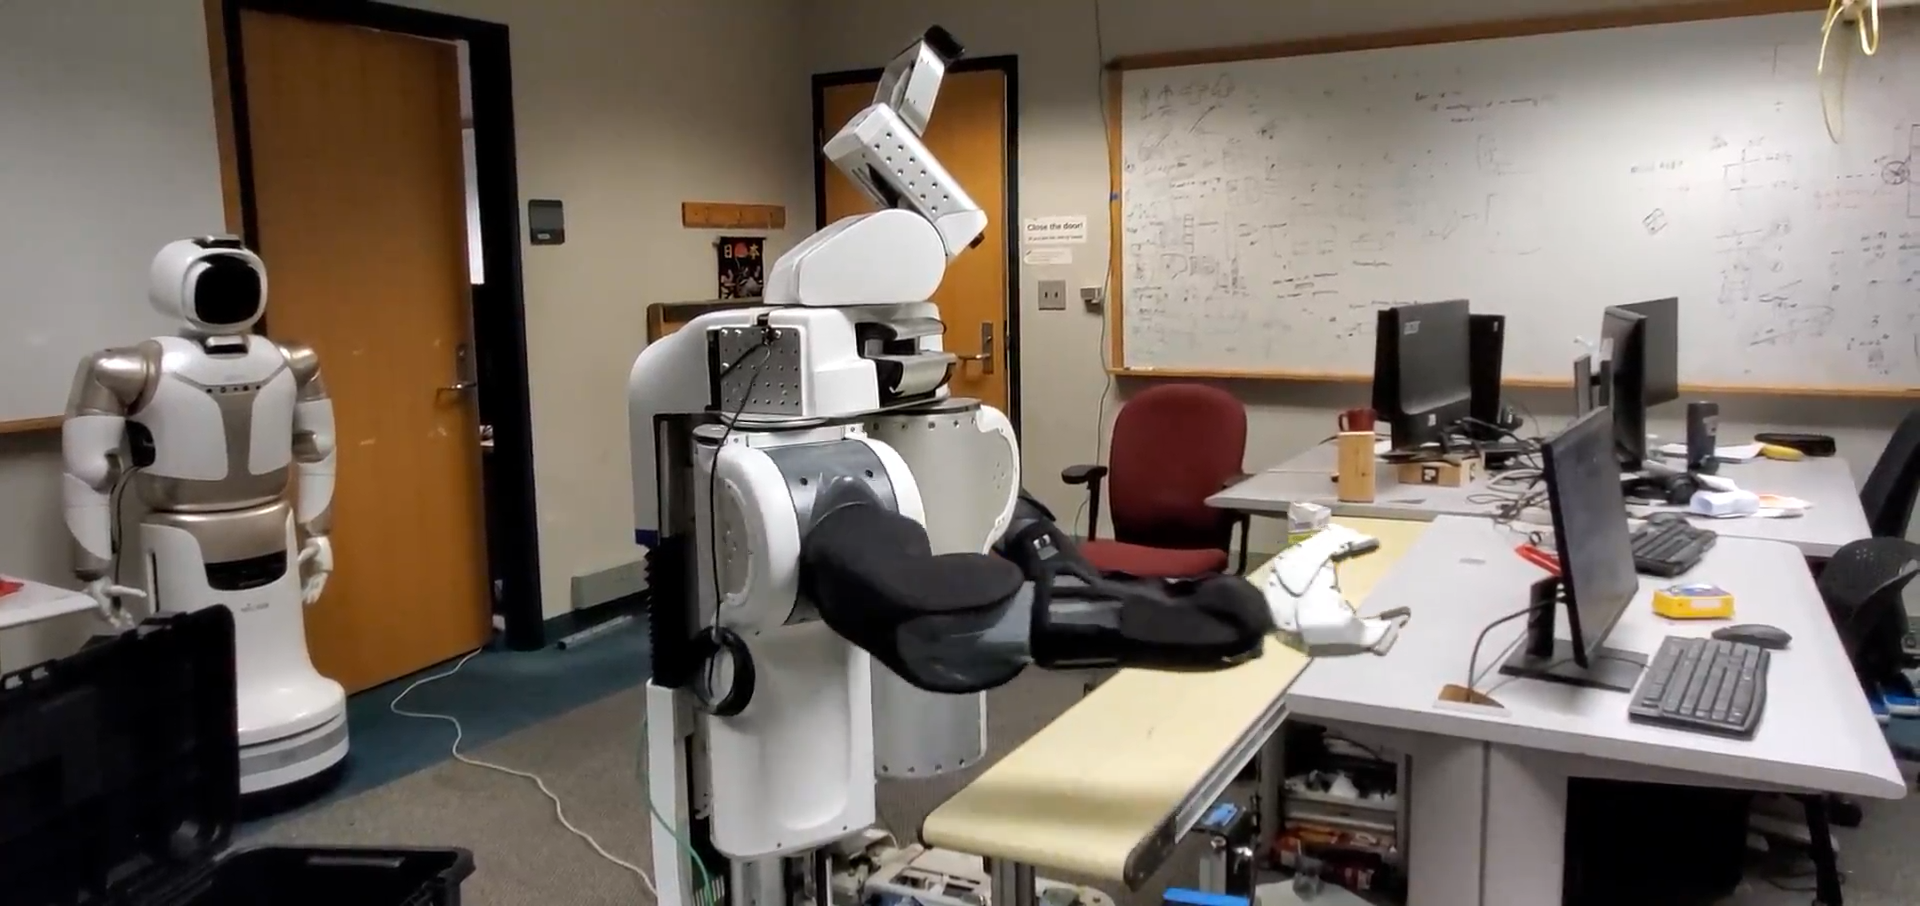
\includegraphics[width=\textwidth]{3.pdf}
        \caption{}
        \label{fig:p2}
    \end{subfigure}
    \begin{subfigure}{0.48\textwidth}
    %   \centering
        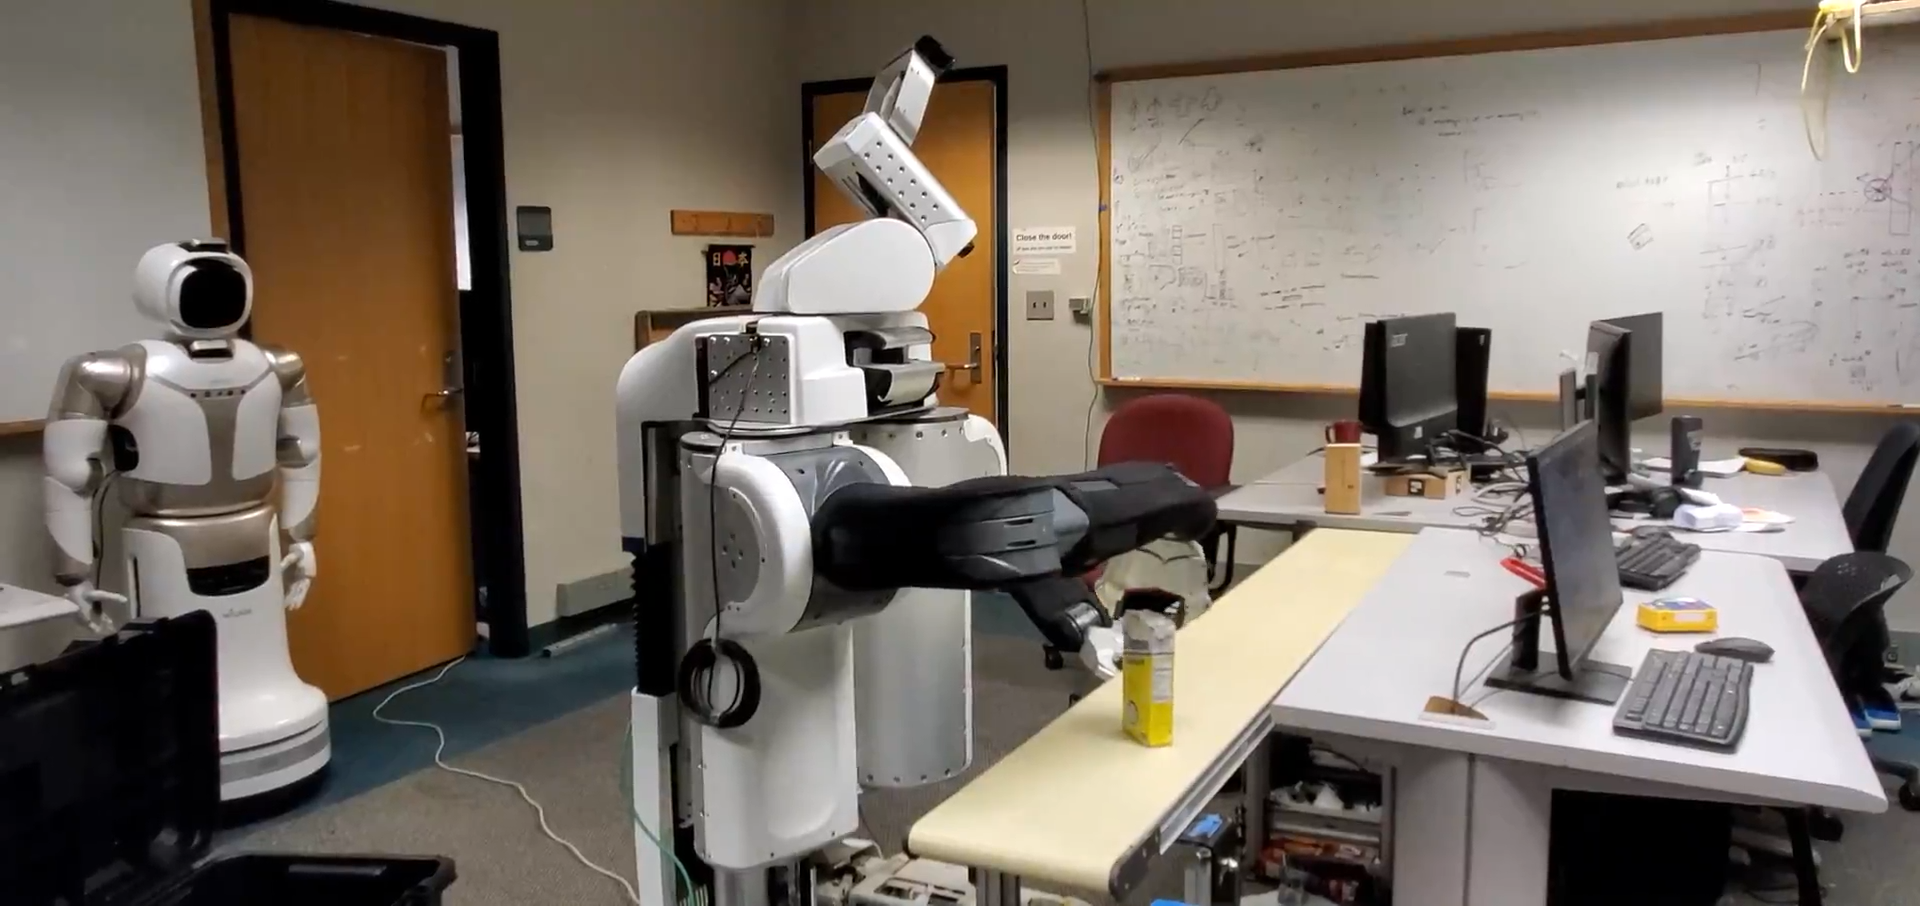
\includegraphics[width=\textwidth]{4.pdf}
        \caption{}
        \label{fig:p3}
    \end{subfigure}
    \begin{subfigure}{0.48\textwidth}
    %   \centering
        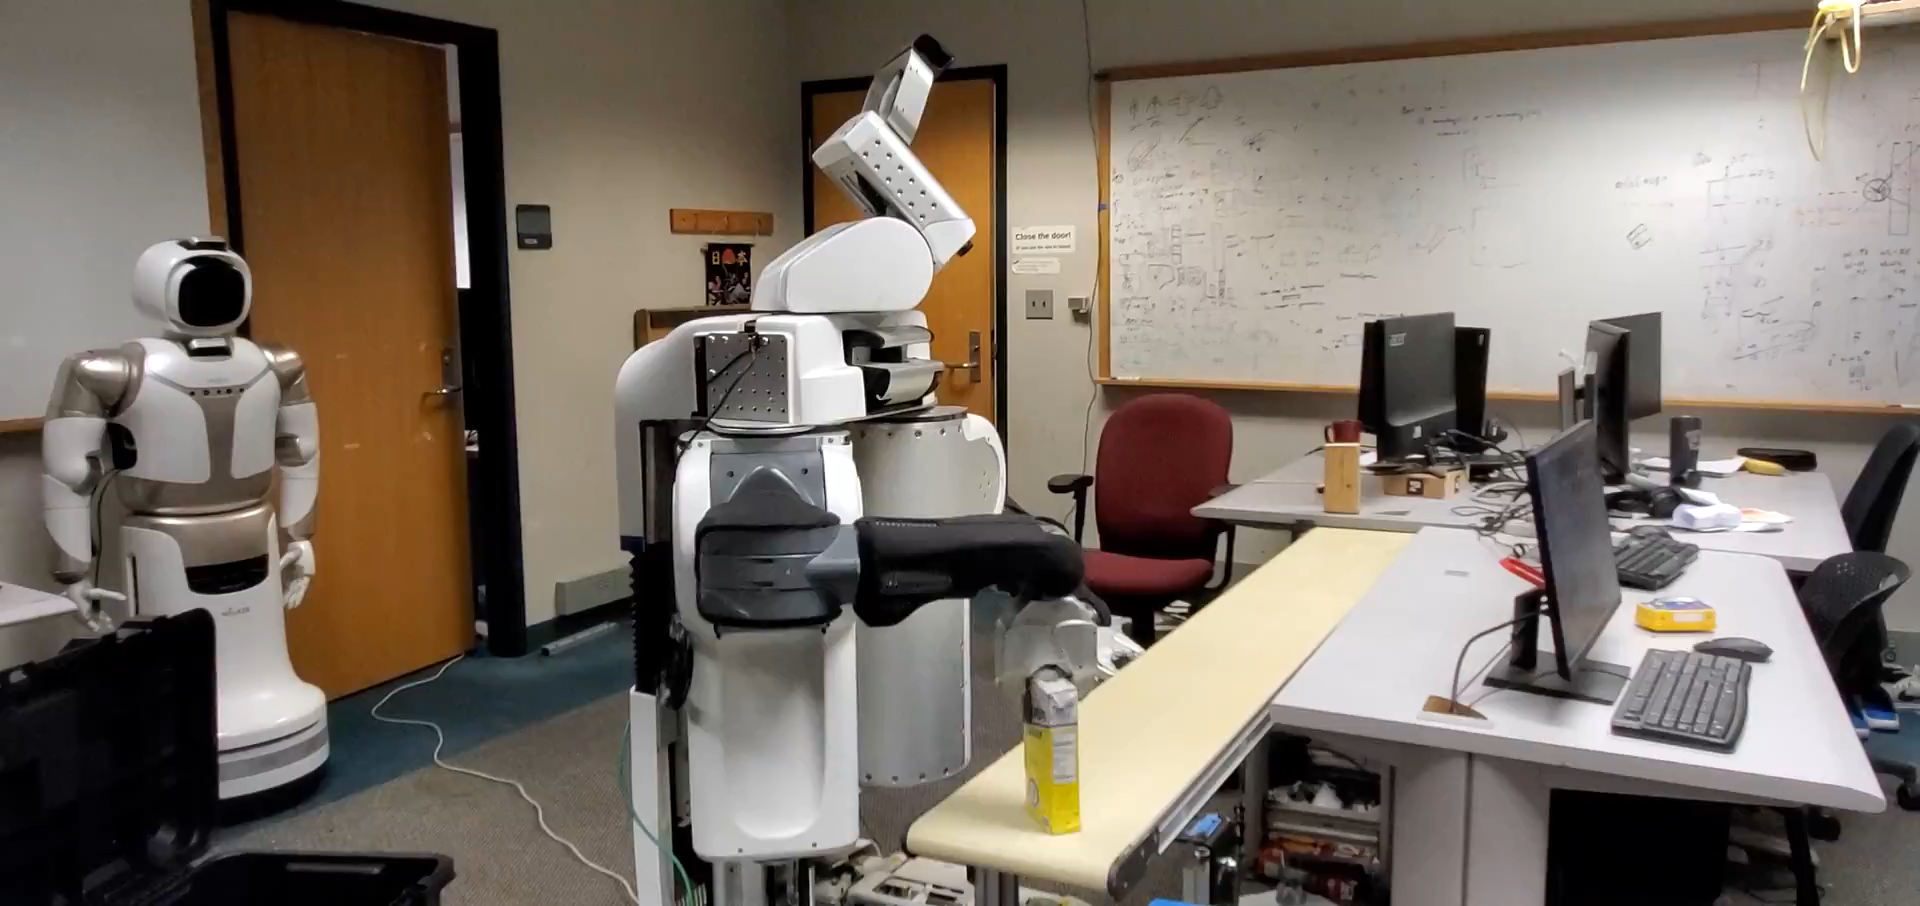
\includegraphics[width=\textwidth]{5.pdf}
        \caption{}
        \label{fig:p4}
    \end{subfigure}
        \begin{subfigure}{0.48\textwidth}
    %   \centering
        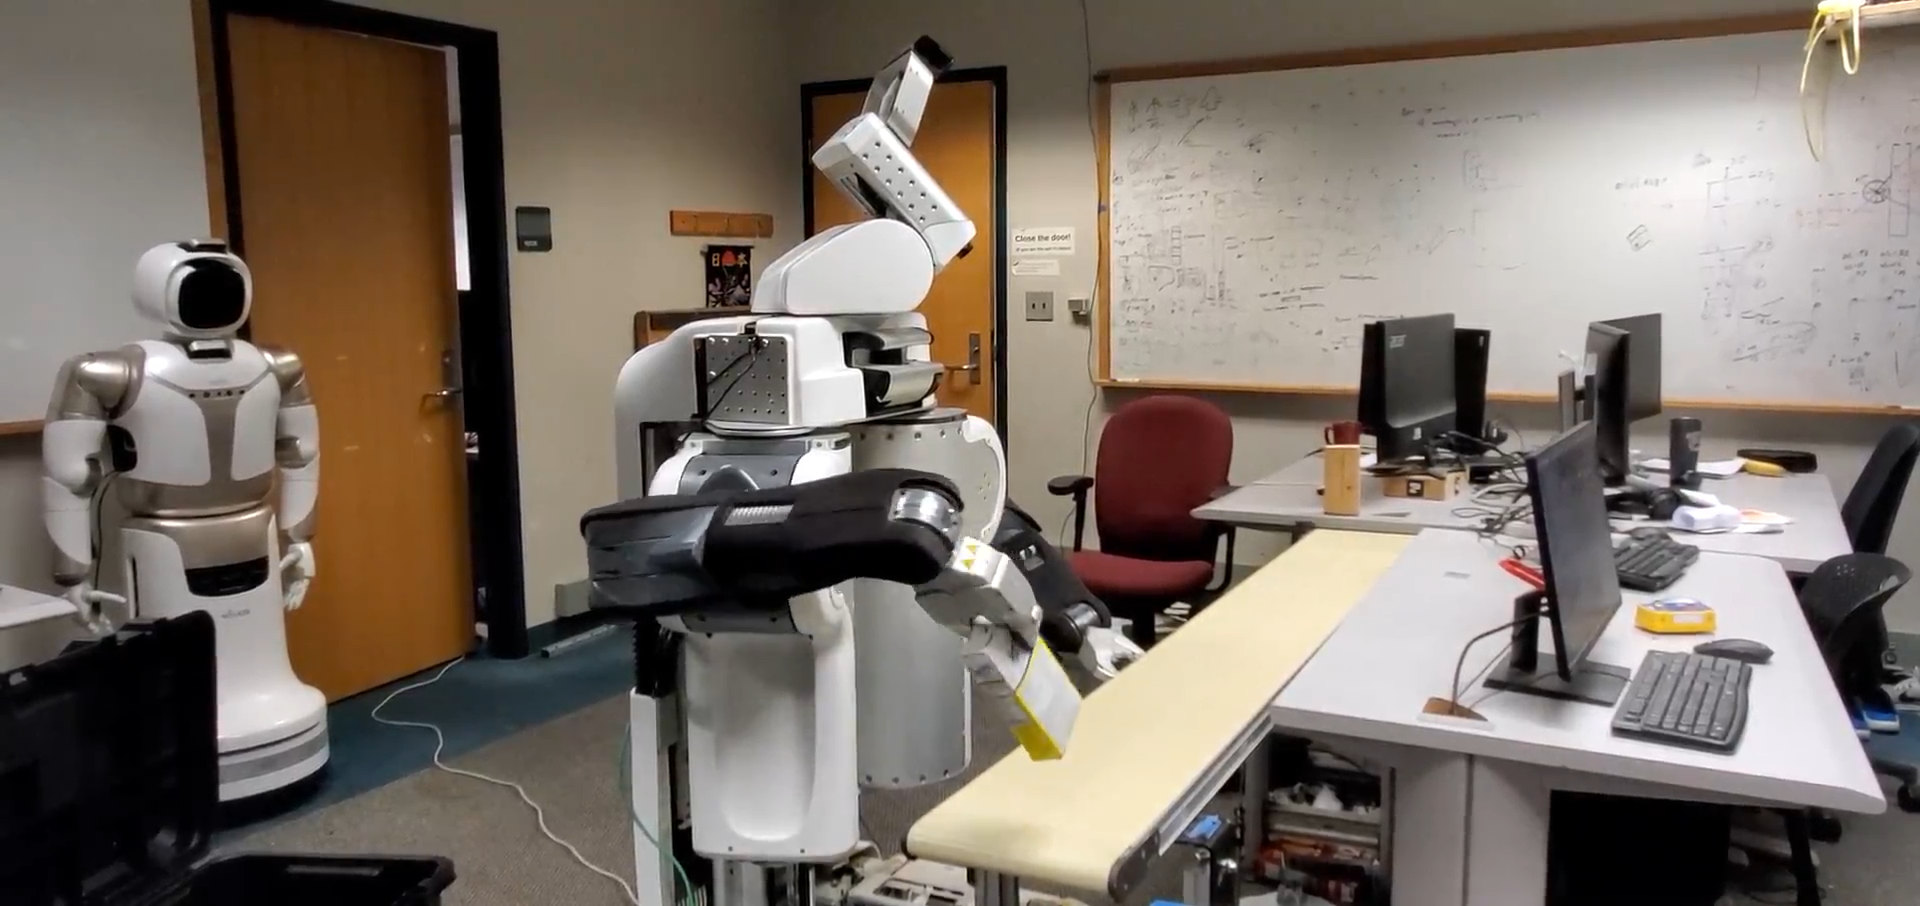
\includegraphics[width=\textwidth]{6.pdf}
        \caption{}
        \label{fig:p5}
    \end{subfigure}
        \begin{subfigure}{0.48\textwidth}
    %   \centering
        \includegraphics[width=\textwidth]{7.pdf}
        \caption{}
        \label{fig:p6}
    \end{subfigure}
        \begin{subfigure}{0.48\textwidth}
    %   \centering
        \includegraphics[width=\textwidth]{8.pdf}
        \caption{}
        \label{fig:p7}
    \end{subfigure}
        \begin{subfigure}{0.48\textwidth}
    %   \centering
        \includegraphics[width=\textwidth]{9.pdf}
        \caption{}
        \label{fig:p8}
    \end{subfigure}
    \caption{
    Illustration of preprocessing steps in a 2D environment with two movable obstacles $\{o_1,o_2\} \in \calO$ for a point robot. APP plans a set of paths from \Sstart to $g$ such that for any configuration of $o_1,o_2$ at least one of the paths from the set is collision free. Static obstacles $\calW_S$ are shown in green and $o_1,o_2$ are depicted as circles. The dotted region depicts $\calQ(o_i)$ (identical for $o_1,o_2$). Namely, $o_1,o_2$ are confined within the dotted region.
     (\subref{fig:p1})~APP finds the first path $\pi_1$ avoiding $\calW_S$ only
    %
    (\subref{fig:p2})~Constructs envelope $e_{\pi_1}$ around $\pi_1$. The dark shaded region shows $e_{\pi_1}$ and the light region shows its occupancy.
    %
    (\subref{fig:p3})~Finds second path $\pi_2$ avoiding $e_{\pi_2}$. Since APP successfully finds two disjoint paths at this step, these paths are sufficient to avoid any configuration of $o_1$.
    %
    (\subref{fig:p4})~Constructs envelope $e_{\pi_2}$ around $\pi_2$.
    %
    (\subref{fig:p5})~Attempts to find the third disjoint path but fails and bisects $e_{\pi_1}$ into $e^l$ and $e^r$.
    %
    (\subref{fig:p6})~Finds path $\pi_3$ around $e^l$ and $e_{\pi_2}$
    %
    (\subref{fig:p7})~Finds path $\pi_4$ around $e^r$ and $e_{\pi_2}$ 
    %
    (\subref{fig:p8})~Set of paths needed to avoid any configuration of $o_1,o_2$.
    }
    
    %
    \label{fig:illustration}
    % \vspace{-4mm}
\end{figure*}

\newlength{\textfloatsepsave}
\setlength{\textfloatsepsave}{\textfloatsep}
\setlength{\textfloatsep}{0pt}
\begin{algorithm}[t]
\caption{\textsc{Preprocess($g$)}} \label{alg1}
% \AlgFontSize

\hspace*{\algorithmicindent} \textbf{Inputs:} $\Sstart, \calW_S, \calO$

\hspace*{\algorithmicindent} \textbf{Output:} $\Pi_g$
\begin{algorithmic}[1]
\State $\pi_1 \leftarrow$ \textsc{FindPath}($\Sstart,g,\calW_S$)
\State $\calE_{\pi_1} \leftarrow \emptyset$
\State \textsc{SetAvoidedEnvelopesOfPath($\pi_1,\calE_{\pi_1}$)}
\State $\Pi_1 \leftarrow \{\pi_1\}$
% \State $\calE \leftarrow \emptyset$
\State $\Pi_g \leftarrow \Pi_1$
\For {$i = 1$ to $n$}  \Comment{$n = |\calO|$}  \label{alg1:l1}
    \State $\Pi_{i+1} \leftarrow \emptyset$
    \For{each $\pi_j \in \Pi_i$} \label{alg1:l2}
    \State $e_{\pi_j} \leftarrow$ \textsc{ConstructEnvelope($\pi_j$)}
    % \State $\calE \leftarrow \calE \cup \{e\}$
    % \State $\Pi_{i+1} \leftarrow$ 
    % \For{each $e \in \calE_i$}
    \State \textbf{If} $e_{\pi_j} = \emptyset$ \textbf{skip to next iteration}
        \State $\calE_{\pi_j} \leftarrow$ \textsc{GetAvoidedEnvelopesOfPath}($\pi_j$)
        \State $\calE_{\pi_j'} \leftarrow \calE_{\pi_j} \cup \{e_{\pi_j}\}$
        % \State $\pi_j' \leftarrow$ \textsc{FindPathAroundEnvelopes}($\calE_{\pi_j'}$)
        \State $\pi_j' \leftarrow$ \textsc{FindPath}($\Sstart,g,\calW_S,\calE_{\pi_j'}$) \Comment{Avoiding $\calE_{\pi_j'}$}
        \If{success}
            \State \textsc{SetAvoidedEnvelopesOfPath($\pi_j', \calE_{\pi_j'}$)}
            % \State \textbf{insert} $<e_{\pi_j}, \pi_j>$ in $\calD_g$
            \State $\Pi_{i+1} \leftarrow \Pi_{i+1} \cup \{\pi_j'\}$
        \Else
            \State $\Pi_{i+1} \leftarrow \Pi_{i+1} \cup \textsc{BisectAndFindMorePaths}(\calE_{\pi_j'})$ \label{alg1:bisect}
            % \State update $\calE_i$ in \calE
            % \State $\Pi \leftarrow \Pi \cup \Pi_{i+1}$
    \EndIf
    \EndFor
    \State $\Pi_g \leftarrow \Pi_g \cup \Pi_{i+1}$
\EndFor
% \State $\calD_g = \Pi_1 \cup \Pi_2 \cup ... \cup \Pi_{n+1}$
\end{algorithmic}
\end{algorithm}
\setlength{\textfloatsep}{\textfloatsepsave}


\setlength{\textfloatsepsave}{\textfloatsep}
\setlength{\textfloatsep}{0pt}
\begin{algorithm}[t]
\caption{\textsc{BisectAndFindMorePaths($\calE$)}} \label{alg2}
% \AlgFontSize
\begin{algorithmic}[1]
    \State $\Pi \leftarrow \emptyset$
    % \State $\calE_\pi \leftarrow$ \textsc{GetAvoidedEnvelopesOfPath}($\pi$)
    % \State $\calE_\pi \leftarrow \calE_\pi \cup \{e\}$
    \State $e \leftarrow \calE$.pop()     \Comment{pop an envelope to bisect}
    \label{alg2:pop}
    \If {\textsc{CheckSingleton}($e$)}    \Comment{contains one position}
        \State \textbf{return} $\emptyset$  \Comment{no further bisection possible}
    \EndIf
    \State $e^{l},e^{r} \leftarrow$ \textsc{BisectEnvelope($e$)} \label{alg:2:bisect}
    \State $\calE_{\pi_l} \leftarrow \calE \cup \{e^l\}$
    \State $\calE_{\pi_r} \leftarrow \calE \cup \{e^r\}$
    \For {each $\calE_{\pi_i} \in \{\calE_{\pi_l},\calE_{\pi_r}\}$}
    
        % first path
        % \State $\calE_{\pi_b} \leftarrow \calE \cup \{e^b\}$
        \State $\pi_i \leftarrow$ \textsc{FindPath}($\Sstart,g,\calW_S,\calE_{\pi_i'}$) \Comment{Avoiding $\calE_{\pi_i'}$}
        \If{success}
            \State \textsc{SetAvoidedEnvelopesOfPath($\pi_i, \calE_{\pi_i}$)}
            % \State \textbf{insert} $<e_{\pi_j}, \pi_j>$ in $\calD_g$
            \State $\Pi \leftarrow \Pi \cup \{\pi_i\}$
        \Else
            \State $\Pi \leftarrow \Pi \cup \textsc{BisectAndFindMorePaths}(\calE_{\pi_i})$
        \EndIf
    \EndFor
    % \State $\calE_s \leftarrow \calE_s \cup \{\tau_{a},\tau_{b}\}$
    \State \textbf{return} $\Pi$
    
    % \For {}
% \EndFor
\end{algorithmic}
\end{algorithm}
\setlength{\textfloatsep}{5pt}

\subsubsection{Query}
A query is comprised of a goal $g \in G$ (\Sstart is fixed) and obstacle configurations $q(o_1) \in Q(o_1), q(o_2) \in Q(o_2),..., q(o_n) \in Q(o_n)$. The query phase first looks up the datastructures stored for the queried $g$. It then loops over the set of paths $\Pi_g$ until it finds a collision free path. It is important to note that while doing so, it does not require any collision checking, which typically is the most computationally expensive operation in motion planning. Instead, it uses the envelope $e_{\pi_j}$ of each path $\pi_j$ to find the collision free path. The following data structures are stored for the query phase to efficiently return collision free paths.
\begin{center}
\begin{tabular}{l}
    $\calM : \; [G \rightarrow \{\calD_{g_1}, \calD_{g_2},...\}]$ \\
    $\calD_{g_i} : \; <\{e_{\pi_1},e_{\pi_2},...\} : \{\pi_1,\pi_2,...\}>$ \Comment{for each $g_i \in G$}\\
    % $\calM_e : Q(o_i) \rightarrow \{e_{\pi_1},e_{\pi_2},...\}$ \Comment{for each envelope}\\
\end{tabular}{}
\end{center}

Namely, $\calM$ is a lookup table that maps a goal~$g_i \in G$ to a dictionary~$\calD_{g_i}$ where ~$\calD_{g_i}$ contains $<e_{\pi_j},\pi_j>$ pairs where $\pi_j \in \Pi_{g_i}$. The query phase is a straight-forward two step process; in the first step, the dictionary~$\calD_{g_i}$ is fetched for the queried $g_i$ from $\calM$. In the second step, the algorithm loops through all the pairs in $\calD_{g_i}$ to search for an envelope $e_{\pi_j}$ that \emph{does not} contain any of the obstacle configurations i.e. $e_{\pi_j} | q(o_1),q(o_2),...,q(o_n) \notin e_{\pi_j}$ in the given planning query. By construction of the preprocessing algorithm, atleast one of the envelopes in $\calD_{g_i}$ is guaranteed to satisfy this condition.  To efficiently check whether a configuration is contained in an envelope or not, we store envelopes as hash tables, which allows the algorithm to perform this check in constant time.

\section{Analysis}
\subsection{Time Complexity}
\label{sec:complexity_app}
\begin{lemma}[Fixed-time query]
The query time of APP is upper-bounded by a (small) time limit $t_{\textrm {query}}$.
\label{lemma1}
\end{lemma}
\begin{proof}[Sketch of Proof]
The query phase includes a lookup operation on \calM, running a loop over the set of alternative paths $\Pi_g$ to the queried $g$ and a nested loop through \calO which also only involves lookup operations since the envelopes are stored as sets. Since with perfect hashing (~\cite{czech1997perfect}), the lookup operations can be performed in constant time. The overall complexity thus is bounded and is given by $O(|\Pi_g|\cdot |\calO|)$ which bounds $t_{\textrm {query}}$.
\end{proof}

\textbf{Special case:} When all paths in $\Pi_g$ are disjoint, then we have that $|\Pi_g| \leq n+1$ and so the complexity of the query phase becomes $O(|\calO|^2)$

In practice we have that $|\Pi_g| \ll Q(o_1) \times Q(o_2) \times ... \times Q(o_n)$ (number of paths required for the naive approach) and therefore, $t_{\textrm {query}}$ is very small.

\subsection{Correctness}
\begin{lemma}
\label{lemma:complete_app}
If the offline motion planner \calP can find a collision-free path from \Sstart to a $g \in G$ in a (large) timeout $t_{\textrm preprocess}$, then APP is guaranteed to generate a path for the same planning problem in time $t_{\textrm {query}}$.
\end{lemma}
\begin{proof}[Sketch of Proof]
For the special case when all paths in $\Pi_g$ are disjoint, the proof follows from Def.~\ref{def:disjointness} because, since the envelopes of paths in $\Pi_g$ are disjoint sets, no obstacle configuration $q(o_i)$ can intersect with more than one path in $\Pi_g$. Since the algorithm computes $n+1$ paths if required for $n$ obstacles, at least one path is collision free.

For the general case where not all paths in $\Pi_g$ are necessarily disjoint, the lemma can be proven by assessing the recursive bisection procedure in APP. In the Alg.~\ref{alg1}, \calP attempts to find the ($n+1$)th path which avoids $n$ envelopes and bisects one of the $n$ envelopes if \calP fails within $t_{\textrm {preprocess}}$. The bisection occurs recursively until either the path is computed for every leaf envelope or further recursion is not possible, thus covering all possible configurations of obstacles in \calO. Since APP uses \calP with the timeout $t_{\textrm {preprocess}}$ to solve each problem, it guarantees to have precomputed a valid path for any problem that \calP can solve in $t_{\textrm {preprocess}}$.
Furthermore from Lemma~\ref{lemma1}, we have that the query time is guaranteed to be within $t_{\textrm {query}}$.
\end{proof}

\subsection{CTMP-Completeness}
We now analyse the algorithm under the CTMP-Completeness criteria described in chapter~\ref{sec:ctmp} for the special case described in Sec.~\ref{sec:complexity_app} when all paths in $\Pi_g$ are disjoint. For the general case, we observe that $|\Pi_g|$ is unbounded (the worst case analysis of $|\Pi_g|$ is outside the scope of this thesis). However, for the special case, we showed that the complexity of the query phase becomes $O(|\calO|^2)$. In addition, if we make the assumption that the maximum number of movable obstacles $\calO$ is a constant, the complexity then becomes $O(1)$.
%
Since the algorithm requires~$O(1)$ time to generate the full path, it would also require~$O(1)$ time to get the next action along the path. Therefore, $T_\textrm{const} (< \Tbound)$ is constant-time bounded. Furthermore, we select the motion planner \calP such that the planned paths contain no cycles. Hence from lemma~\ref{lemma:complete_app} and by Def.~\ref{def:complete}, we have the following theorem.

\vspace{2mm}
\begin{theorem}
	For the case when all paths in $|\Pi_g|$ are disjoint, the algorithm is CTMP-Complete under the assumption that $|\calO|$ is upper-bounded by a constant.
\end{theorem}

\section{Implementation Details} % : Motion Planning for Robot Arm}
%In this section we cover two main components of our approach specifically for the motion planning problem for a high-DoF robot arm, (1) envelope construction and (2) envelope bisection.
In this section we cover three main components of our implementation for the motion planning problem of a high-DoF robot arm, (1) envelope construction, (2) envelope bisection and (3) computing envelope occupancy.
%
Our implementation approximates the geometry of the movable obstacles with spheres. This approximation restricts the dimensionality of $Q(o_i)$ to $\mathbb{R}^3$.


\subsection{Envelope Computation using Distance Field}
\label{sec:impl_details}
The naive approach of computing an envelope $e_\pi$ around a path $\pi$ (recall Def.~\ref{def:envp}) requires collision checking all obstacle configurations with each robot state $s \in \pi$. This can be very expensive for a large number of configurations that the obstacles can have.
% To optimize this computation, we approximate an obstacle $o_i$ with a sphere of radius $r_i$, which allows us to efficiently perform this computation using a distance field.
% Recall Def.~\ref{def:envp} of the envelope. The naive approach of constructing an envelope $e_\pi$ for a path $\pi$ is to make use of a collision checker for the robot and find the set of all configurations of all obstacles $o_i \in \calO$ that collide with any configuration of the robot along~$\pi$. This would require~$|\pi| \times Q(o_1) \times Q(o_2) \times ... \times Q(o_n)$ collision checks, where $|\pi|$ is the length of $\pi$. This clearly is prohibitive to compute, even offline.
%
% To optimize for the preprocessing computation, we make the following simplistic assumption.
%
% % \begin{assumption}
% % \label{assum:1}
% % We assume that all obstacles $o_i \in \calO$ are identical in geometry.
% % \end{assumption}
%
% % For the naive approach, this now requires~$|\pi| \times Q(o_i)$ collision checks which still is not affordable. To this end we make another assumption~\ref{assum:2}.
%
% \begin{assumption}
% \label{assum:2}
% We approximate the geometry of each obstacles $o_i \in \calO$ by a sphere of radius $r_i$.
% \end{assumption}
%
% This allows us to use a method for envelope construction that does not require the expensive collision checking. With the spherical approximation, we now refer to obstacle configurations as positions in the 3D world.
%
Instead, the envelope is constructed in a simple two step process.
%\begin{enumerate}
First, the path $\pi$ is voxelized (using the collision model of the robot) and added to an occupancy grid.
% This is done by converting the collision model of the robot at each configuration $s \in \pi$ to voxels and inserting them in the occupancy grid.
Second, 
to compute the positions of each $o_i \in \calO$ that collide with $\pi$, the occupancy grid is inflated by the radius~$r_i$ of $o_i$, (approximating an obstacle $o_i$ with a sphere of radius $r_i$) which is efficiently done by using a signed distance field.
%The method iterates through all cells in the occupancy grid and fills the ones which are at most~$r_i$ distance away from the occupied cells.
%
The intersection of the set of discrete positions of the occupied cells with $Q(o_i)$, constitutes $e_{\pi}$.
%\end{enumerate}
%
To allow computing disjoint paths, following Def.~\ref{def:envp}, the obstacle positions that collide with \Sstart or are within a small distance $\epsilon$ from the goal position are excluded from $e_\pi$. This enforces an assumption that an obstacle is not placed within $\epsilon$ distance from the goal position.
% By the end of this two step process, the cells that are occupied constitutes~$e_\pi$, i.e. the discrete obstacle positions corresponding to each of these cells, collide with $\pi$.
% (since we assume the same geometrical approximation for all $o \in \calO$)

\subsection{Envelope Bisection}
The envelope bisection refers to splitting an envelope~$e$ into two sub-envelopes~$e_l$ and $e_r$ (see Alg.~\ref{alg2} line~\ref{alg:2:bisect}). Several schemes could be used to make this split. In our implementation, we split the envelope along either of the three planes $x=x_c, y=y_c$ or $z=z_c$. where the $x_c,y_c$ and $z_c$ are the means of the $x,y$ and $z$ components respectively of all positions in the envelope $e$ to be bisected. Among the three axes, we pick the axis that has the largest span of positions. As described earlier, each envelope is implemented as a binary tree and this bisection results in creation of two children~$e_l$ and~$e_r$ for the parent~$e$ in this binary tree. Note that we remove subscripts for paths once the envelope is bisected since the bisected envelopes no more follow Def.~\ref{def:envp}.
%
Alg.~\ref{alg2} also makes a choice at line~\ref{alg2:pop} for the envelope to be bisected from the input set of envelopes \calE. While this decision does not affect the properties of the algorithm, different heuristics can be used for this choice as well. In our implementation, we simply select the largest envelope for bisection.

\subsection{Computing Envelope Occupancy}
This step corresponds to an implementation detail within procedure \textsc{FindPath} in Alg.~\ref{alg1}. In order to find a path around the set of envelopes \calE, the joint occupancy of all envelopes in \calE is computed. To do so, for each obstacle $o_i$, all of its discrete positions in \calE are added to an empty occupancy grid, followed by the inflation of the occupancy grid (as described earlier) by the radius $r_i$ of the corresponding obstacle $o_i$. The joint occupancy of all these grids constitutes the occupancy of \calE.
%
%
\footnote{In our experiments, we consider all obstacles of the same sizes. In that case, a single inflation operation is needed, each for the envelope construction and computing envelope occupancy steps.}

\begin{figure*}[t]
    \centering
    \begin{subfigure}{0.48\textwidth}
    %   \centering
        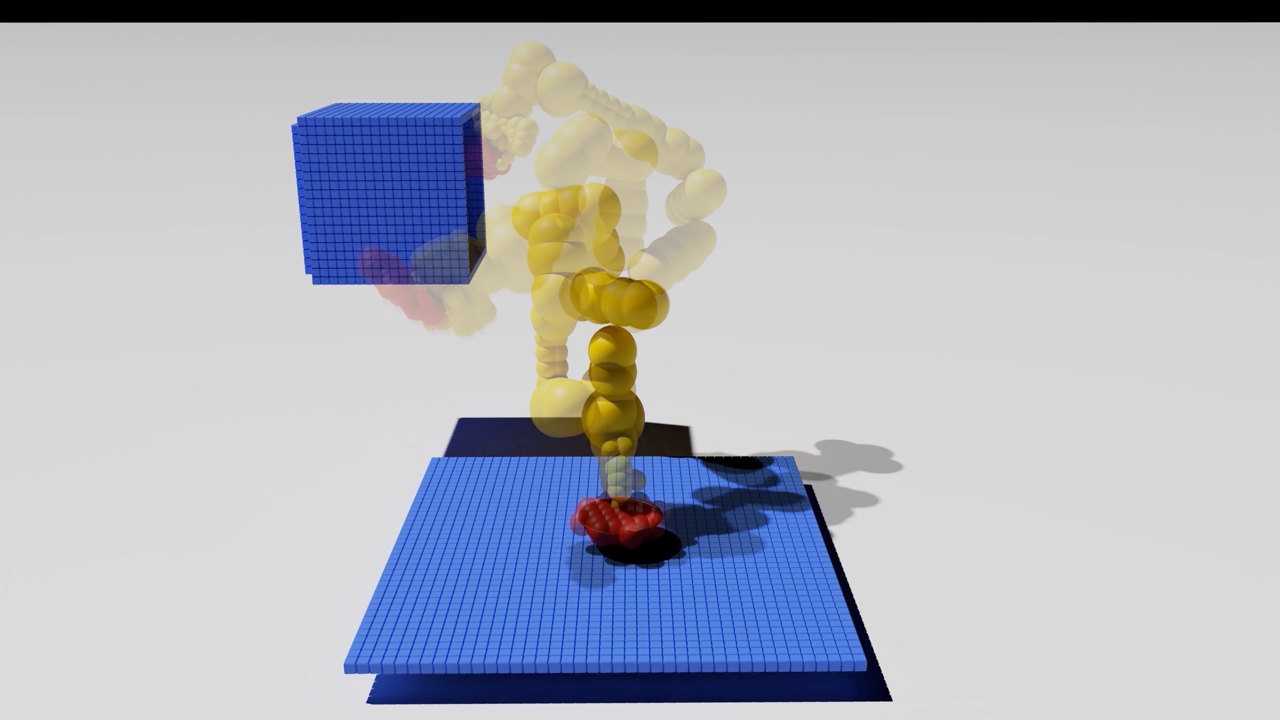
\includegraphics[trim={8cm 0 10cm 1cm},clip, width=\textwidth]{path1.png}
        \caption{}
        \label{fig:pr1}
    \end{subfigure} 
    \begin{subfigure}{0.48\textwidth}
    %   \centering
        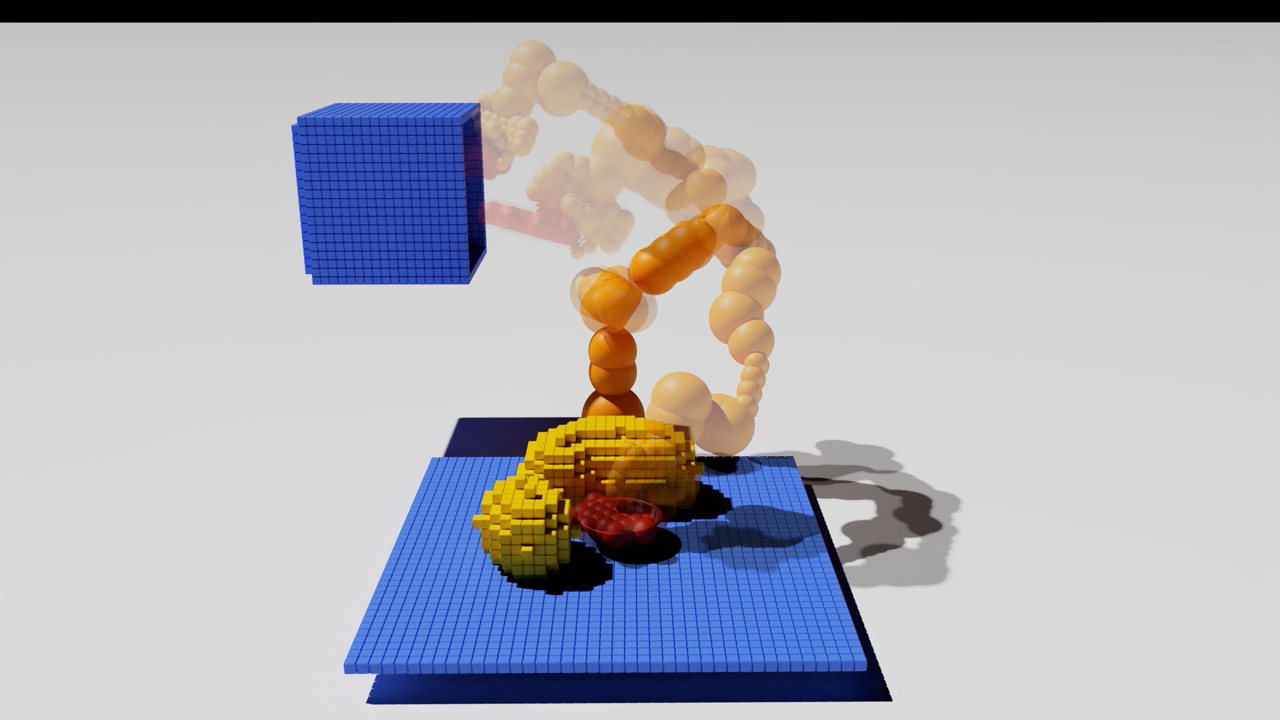
\includegraphics[trim={8cm 0 10cm 1cm},clip, width=\textwidth]{path2.png}
        \caption{}
        \label{fig:pr2}
    \end{subfigure}
    \begin{subfigure}{0.48\textwidth}
    %   \centering
        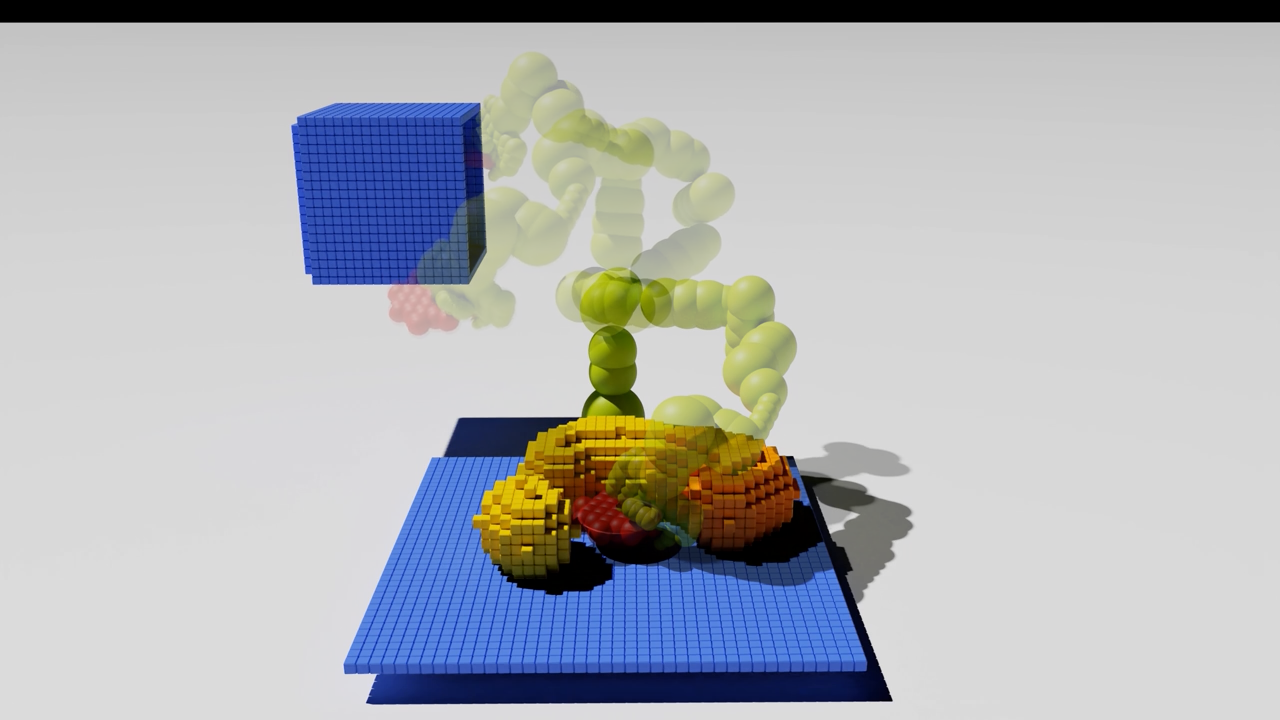
\includegraphics[trim={8cm 0 10cm 1cm},clip, width=\textwidth]{path3.png}
        \caption{}
        \label{fig:pr3}
    \end{subfigure}
    \begin{subfigure}{0.48\textwidth}
    %   \centering
        \includegraphics[trim={8cm 0 10cm 1cm},clip, width=\textwidth]{path4.png}
        \caption{}
        \label{fig:prq}
    \end{subfigure}
    \caption{
    Illustration of the preprocessing steps for the mail-sorting environment with two movable obstacles on a tabletop for a single start and goal pair.
     (\subref{fig:pr1})~APP finds the first path avoiding $\calW_S$ only.
    %
    (\subref{fig:pr2})~Constructs envelope around first path and finds the second path avoiding the first envelope.
    %
    (\subref{fig:pr3})~Constructs a second envelope around the second path and finds the third path avoiding the two envelopes.
    %
    (\subref{fig:prq})~At query time, given a random configuration of movable obstacles, APP looks up a valid path~(second path, Fig.~\subref{fig:pr2}) among the set of precomputed paths.
    }
    %
    \label{fig:pr}
    % \vspace{-4mm}
\end{figure*}

\section{Experimental Results}

\begin{table*}[tbh!]
\footnotesize
\begin{center}
\begin{adjustbox}{angle=-90}
\begin{tabular}{|r|r||c|c|c|c|c|c|c|c|c|}
\hline
\multicolumn{2}{|l|}{} & \multicolumn{3}{c|}{Shelving} & \multicolumn{3}{c|}{Sorting} & \multicolumn{3}{c|}{Sorting (time constrained)} \\
\multicolumn{2}{|l|}{} & \multicolumn{3}{c|}{\scriptsize{[248 goals]}} & \multicolumn{3}{c|}{\scriptsize{[680 goals]}} & \multicolumn{3}{c|}{\scriptsize{[680 goals]}} \\
\multicolumn{2}{|r|}{No. of Obstacles} & 1 & 2 & 3 & 1 & 2 & 3 & 1 & 2 & 3 \\ \hline\hline
%%%%%%%%%%%%%%%%%%%  Success Rates
\multirow{7}{*}{\rotatebox[origin=c]{90}{Success Rate [\%]}}
& \textbf{APP}  & \textbf{100}  & \textbf{100}  & \textbf{100}  & \textbf{100}  & \textbf{100}  & \textbf{100}  & \textbf{100}  & \textbf{100}  & \textbf{100} \\ \cline{2-11}
& Lightning~\cite{berenson2012robot}  & 94  & 95  & 97  & \textbf{100}  & \textbf{100}  & \textbf{100}  & 97  & 96  & 75 \\ \cline{2-11}
& E-Graphs~\cite{Phillips-RSS-12}  & 20  & 15  & 14  & 89  & 89  & 81  & 50  & 45  & 41 \\ \cline{2-11}
& RRTConnect~\cite{kuffner2000rrt}  & 96  & 95  & 97  & \textbf{100}  & \textbf{100}  & \textbf{100}  & 19  & 14  & 11 \\ \cline{2-11}
& LazyPRM~\cite{kavraki2000path}  & 46  & 34  & 23  & 98  & 99  & 93  & 46  & 35  & 28 \\ \cline{2-11}
& BIT\textsuperscript{\textasteriskcentered}~\cite{gammell2020batch}  & 92  & 75  & 64  & 84  & 81  & 75  & 37  & 42  & 40 \\ \cline{2-11}
% & InformedRRT\textsuperscript{\textasteriskcentered}~\cite{gammell2018informed}  & 6  & 11  & 12  & \textbf{100}  & \textbf{100}  & \textbf{100}  & 25  & 23  & 16 \\ \cline{2-11}
& RRT\textsuperscript{\textasteriskcentered}~\cite{karaman2011sampling}  & 9  & 12  & 17  & \textbf{100}  & \textbf{100}  & \textbf{100}  & 20  & 15  & 25 \\ \hline\hline
%%%%%%%%%%%%%%%%%%%  Planning Times
\multirow{14}{*}{\rotatebox[origin=c]{90}{Mean Time (std, max) [ms]}}
& \multirow{2}{*}{\textbf{APP}}  & \textbf{.005}  & \textbf{.006}  & \textbf{.006}  & \textbf{.005}  & \textbf{.005}  & \textbf{.007}  & \textbf{.005}  & \textbf{.005}  & \textbf{.006} \\
&  & \scriptsize{(.001, .009)} & \scriptsize{(.001, .013)} & \scriptsize{(.001, .014)} & \scriptsize{(.001, .008)} & \scriptsize{(.001, .009)} & \scriptsize{(.001, .011)} & \scriptsize{(.001, .009)} & \scriptsize{(.001, .009)} & \scriptsize{(.001, .008)}\\ \cline{2-11}
& \multirow{2}{*}{Lightning~\cite{berenson2012robot}}  & 124  & 149  & 162  & 31.1  & 37.5  & 48.6  & 70.7  & 77.5  & 98.4 \\
&  & \scriptsize{(28.2, 221)} & \scriptsize{(63.3, 413)} & \scriptsize{(82.2, 552)} & \scriptsize{(13.7, 76.8)} & \scriptsize{(20.0, 96.1)} & \scriptsize{(30.2, 144)} & \scriptsize{(80.3, 542)} & \scriptsize{(63.0, 307)} & \scriptsize{(84.6, 414)}\\ \cline{2-11}
& \multirow{2}{*}{E-Graphs~\cite{Phillips-RSS-12}}  & 988  & 1044  & 904  & 203  & 273  & 275  & 162  & 210  & 176 \\
&  & \scriptsize{(587, 1943)} & \scriptsize{(484, 1952)} & \scriptsize{(364, 1520)} & \scriptsize{(92.0, 824)} & \scriptsize{(290, 1936)} & \scriptsize{(250, 1918)} & \scriptsize{(55.2, 534)} & \scriptsize{(78.1, 575)} & \scriptsize{(78.6, 567)}\\ \cline{2-11}
& \multirow{2}{*}{RRTConnect~\cite{kuffner2000rrt}}  & 168  & 167  & 260  & 62.0  & 59.5  & 72.9  & 112  & 110  & 104 \\
&  & \scriptsize{(192, 1880)} & \scriptsize{(71.7, 488)} & \scriptsize{(228, 1363)} & \scriptsize{(46.7, 364)} & \scriptsize{(29.2, 151)} & \scriptsize{(38.1, 194)} & \scriptsize{(75.0, 311)} & \scriptsize{(71.6, 272)} & \scriptsize{(72.4, 279)}\\ \cline{2-11}
& \multirow{2}{*}{LazyPRM~\cite{kavraki2000path}}  & 1014  & 1204  & 1196  & 338  & 480  & 442  & 219  & 219  & 224 \\
&  & \scriptsize{(388, 1921)} & \scriptsize{(410, 1954)} & \scriptsize{(516, 1967)} & \scriptsize{(265, 1454)} & \scriptsize{(402, 1716)} & \scriptsize{(405, 1919)} & \scriptsize{(65.8, 386)} & \scriptsize{(72.6, 478)} & \scriptsize{(93.1, 568)}\\ \cline{2-11}
& \multirow{2}{*}{BIT\textsuperscript{\textasteriskcentered}~\cite{gammell2020batch}}  & 727  & 904  & 833  & 327  & 298  & 442  & 251  & 262  & 252 \\
&  & \scriptsize{(256, 1997)} & \scriptsize{(380, 1950)} & \scriptsize{(363, 1923)} & \scriptsize{(357, 1963)} & \scriptsize{(305, 1555)} & \scriptsize{(417, 1728)} & \scriptsize{(102, 556)} & \scriptsize{(92.9, 540)} & \scriptsize{(109, 633)}\\ \cline{2-11}
% & \multirow{2}{*}{InformedRRT\textsuperscript{\textasteriskcentered}~\cite{gammell2018informed}}  & 515  & 546  & 562  & 136  & 136  & 139  & 178  & 190  & 171 \\
% &  & \scriptsize{(76.4, 617)} & \scriptsize{(69.8, 634)} & \scriptsize{(28.6, 603)} & \scriptsize{(31.6, 201)} & \scriptsize{(31.5, 203)} & \scriptsize{(33.1, 209)} & \scriptsize{(44.0, 267)} & \scriptsize{(50.4, 323)} & \scriptsize{(43.4, 253)}\\ \cline{2-11}
& \multirow{2}{*}{RRT\textsuperscript{\textasteriskcentered}~\cite{karaman2011sampling}}  & 572  & 539  & 566  & 137  & 137  & 137  & 193  & 187  & 193 \\
&  & \scriptsize{(128, 893)} & \scriptsize{(54.6, 616)} & \scriptsize{(29.0, 617)} & \scriptsize{(31.9, 196)} & \scriptsize{(31.7, 199)} & \scriptsize{(32.4, 214)} & \scriptsize{(50.3, 289)} & \scriptsize{(36.7, 261)} & \scriptsize{(50.5, 290)}\\ \hline\hline
%%%%%%%%%%%%%%%%%%%  APP Preprocessing
\multirow{6}{*}{\rotatebox[origin=c]{90}{APP}}
& Preprocessing & \multirow{2}{*}{8.9} & \multirow{2}{*}{48.2} & \multirow{2}{*}{49.9} & \multirow{2}{*}{17.6} & \multirow{2}{*}{31.2} & \multirow{2}{*}{74.6} & \multirow{2}{*}{17.5} & \multirow{2}{*}{30.4} & \multirow{2}{*}{98.8} \\
& Time [min] & & & & & & & & & \\ \cline{2-11}
& Paths per Goal & \multirow{2}{*}{2.0 ({0.1})} & \multirow{2}{*}{3.2 ({0.7})} & \multirow{2}{*}{4.1 ({0.9})} & \multirow{2}{*}{2.0 ({0.0})} & \multirow{2}{*}{3.1 ({0.5})} & \multirow{2}{*}{6.1 ({4.0})} & \multirow{2}{*}{2.0 ({0.1})} & \multirow{2}{*}{3.1 ({0.4})} & \multirow{2}{*}{5.8 ({7.7})} \\
& (mean, std)& & & & & & & & & \\ \cline{2-11}
& \multirow{2}{*}{Memory [Mb]} & \multirow{2}{*}{9.7} & \multirow{2}{*}{15.6} & \multirow{2}{*}{20.6} & \multirow{2}{*}{24.8} & \multirow{2}{*}{37.8} & \multirow{2}{*}{70.6} & \multirow{2}{*}{17.5} & \multirow{2}{*}{28.5} & \multirow{2}{*}{54.7} \\
& & & & & & & & & & \\ \hline
\end{tabular}
\end{adjustbox}
\end{center}
\caption{
The table shows the success rates and planning times of APP and the baselines, as well as the preprocessing statistics for three different domains, with 1, 2 and 3 movable obstacles. 100 random tests were run for each experiment with the timeout of 2s. The same timeout was used for APP during preprocessing.
}
\label{table:results}
% \vskip -0.5cm
\end{table*}

\begin{figure}
\centering
\includegraphics[width=\textwidth]{figs/app_fig3_v2_lo-res.png}
\caption{Left: Shelving/unshelving task. Right: mail sorting task. Both tasks involve a mix of static obstacles and obstacles which may appear at many different positions. Target object is shown in red, and approximate movable obstacles are shown in yellow. The goal regions are depicted with green rectangles.}
\label{fig:scenarios}
% \vskip -0.5cm
\end{figure}

We evaluated APP on the 7 DoF Franka arm in three different semi-structured domains and compared its performance with other state-of-the-art sampling-based and search-based motion planning algorithms. For sampling-based algorithms we used OMPL's implementations~\cite{sucan2012open}

%\subsection{Experimental setup}
%\subsubsection*{Manipulation Planning}
%We consider the manipulation planning problem as joint motion and grasp planning problem. Namely,
We consider the problem of reaching a feasible grasp pose $\phi \in \Phi$ for a target object $o_T$ at configuration $q(o_T)$, where $\Phi$ is a set of precomputed grasps (transformed into the robot's frame) for $o_T$. The resultant problem is a multi-goal planning problem where given $\Phi$, the robot has to find a collision free path $\pi$ to any $\phi \in \Phi$ while avoiding obstacles in \calW and meeting the success criterion. We use YCB objects~\cite{calli2015ycb} as targets with the grasps from~\cite{eppner2019billion}.

In all our experiments, we sort the grasp poses using a distance metric selecting the next best grasp being the one closest to the grasps already attempted so far. We use collision-aware IK to find valid grasps. For the baselines that support multi-goal planning (RRT*~\cite{karaman2011sampling}, BIT*~\cite{gammell2020batch}, LazyPRM~\cite{kavraki2000path}) in OMPL, the planner picks the top five grasps from the sorted list and plans to the corresponding goals within a single planning query. For the remaining baselines (Lightning~\cite{berenson2012robot}, RRT-Connect~\cite{kuffner2000rrt}, E-graphs~\cite{Phillips-RSS-12}) the planner sequentially iterates through all the grasps in $\Phi$ and terminates when the success criterion is met or until the timeout. APP uses Lightning as its underlying motion planner \calP.

%\subsubsection*{Goal Region Specification}
We define the goal region \calG as a space of possible configurations of $o_T$ in the world. \calG is domain specific and depends on the allowable region of $o_T$ in the world as well as the geometry of $o_T$. To give an example, we used the bowl from the YCB dataset as the target object in our experiments. Since it is symmetric about the vertical axis and can rest on a planer surface, that limits the dimension of \calG to $\mathbb{R}^2$. For an object like a mug, its \calG would be in $SE(2)$. \calG is discretized to get a discrete set of poses $G$ of $o_T$.
% The discretization is chosen depending upon the precision required for the given domain.


% We test on four different simulated environments to show our proposed method's superiority over a number of common baselines. Specifically, we compare to RRT-Connect (RRTC)~\cite{kuffner2000rrt}, Lightning~\cite{berenson2012robot}, and Lazy PRM~\cite{}.

% TODO: results tables and experiment descriptions plus images here. 

\subsection{Experimental Scenarios}
Fig.~\ref{fig:scenarios} shows two of our example scenarios. In both the scenarios, we define the goal regions \calG as bounded $x,y$ planes since the target objects that we use are symmetric about the $z$-axis. The obstacle regions $\calQ(o_i)$ are also bounded $x,y$ planes and are identical for all obstacles in \calO.~\calG and $\calQ(o_i)$ both are discretized with a resolution of 2cm. We use occupancy grid to represent the occupancy of \calW which also has a 2cm discretization. The value of parameter $\epsilon$ (defined in Def.~\ref{def:envp}) in all the experiments is 20cm.
%
% We design these scenerios such that if an obstacle is place at every position $q(o_i) \in Q(o_i)$, none of the goals in $G$ is reachable. Without that, the planning problem becomes trivial, since we can treat the resultant \calW as completely static.
%
Table~\ref{table:results} shows the statistical results of all our experiments. The experiments were run on Intel Core i7-7800X CPU @3.5Ghz with 32 GB memory.

APP shows a success rate of 100\% for all the experiments, with several orders of magnitude speedup compared to the baselines. The baselines do well in the sorting domain but they suffer in shelving and the time-constrained sorting domains, which are more challenging.
%
Lightning's lower success rate for the shelving domain compared to APP is because randomly positioned obstacles can potentially create harder planning problems, compared to the problems it solves within the APP framework.
%
Lightning's lower success rate for the time-constrained domain is due to its higher planning time, which makes it harder to satisfy the overall timeout~$t_\textrm{task}$.
%
% \hl{Even though APP uses Lightning as its underlying planner \calP, it achieves 100\% success rate which Lightning fails to achieve}
% \hl{For the time-constrained domain, the baselines show lower success rates due to their higher planning times, which makes it harder to satisfy the overall timeout}~$t_\textrm{task}$.
%
%Also, note that the performance of preprocessing and experience-based planners (LazyPRM, Lightning, E-graphs) drops with the increase in the number of movable obstacles.
The performance of preprocessing and experience-based planners (LazyPRM, Lightning, E-graphs) drops with the increase in the number of movable obstacles.
%
In the time constrained domain, optimal sampling-based planners (RRT*, BIT*) do not perform better than non-optimal planners, because besides being slower, their convergence rate is not as fast as the time bound requires. Secondly more significant cost reduction is achieved by post-processing in our domains, which is used for all the planners.

%%%%%%%%%%%%%%%%%%%%%%%%%%%%%%%%%%%%%%%%%%%%%%%%
\textbf{Shelving/Unshelving:}
 %In the shelving/unshelving scenario, the robot is tasked with reaching out to a target object (soup can in this example from the YCB dataset) placed in the rear section of a shelf, while avoiding other objects arbitrarily located at the front section of the shelf. Conversely the task could be to place the object in the rear section of the shelf. We approximate each $o_i \in \calO$ as a sphere (voxelized) of radius 6cm. The planning problem is challenging because the static shelf and the movable obstacles create narrow passages in the configuration space of the robot. Since the target object is symmetric about the vertical $z$-axis,~\calG is a bounded $x,y$ plane in the rear section of the shelve.
 In the shelving/unshelving scenario, the robot is tasked with reaching a target object placed in the rear section of a shelf while avoiding other objects. % arbitrarily located at the front section of the shelf.
 %Conversely the task could be to place the object in the rear section of the shelf.
 We approximate each $o_i \in \calO$ as a voxelized sphere of radius 6cm.
 This problem is challenging because the movable obstacles create narrow passages in the configuration space of the robot.
 Since the target object is symmetric about the vertical axis,~\calG is a bounded plane in the rear section of the shelve.
 
%%%%%%%%%%%%%%%%%%%%%%%%%%%%%%%%%%%%%%%%%%%%%%%%%%%%%%%%%%%%%%%%%%%%%%%%%%%%%%%
\textbf{Mail Sorting:}
%For the mail-sorting task, the robot picks up packages from a tabletop while avoiding collisions with other packages and sorts them in cubby shelves. We approximate each $o_i \in \calO$ as a sphere (voxelized) of radius 8cm for this task. This problem is challenging because in addition to planning to a grasp pose, the planner needs to search for a valid pregrasp pose which gets harder with more clutter around the target object. Additionally the target cubby creates a narrow passage for the motion planner.
The robot must pick up packages from a tabletop while avoiding collisions with other packages and put them in a cubby. We approximate each $o_i \in \calO$ as a voxelized sphere of radius 8cm. %This problem is challenging because i
In addition to planning to a grasp pose, the planner needs to search for a valid pregrasp pose which gets harder with more clutter around the target object. Additionally, the target cubby creates a narrow passage for the motion planner.
%
An example of the preprocessing phase for a single start and goal pair for this domain is depicted in Fig.~\ref{fig:pr} 
% \begin{figure*}[t]
%     \centering
%     \includegraphics[width=0.5\textwidth]{figs/times_sorting.pdf}
%     \includegraphics[width=0.45\textwidth]{figs/times_shelving.pdf}
%     \caption{Planning times for two use cases: mail sorting (left) and shelving (right).}
%     \label{fig:boxplot}
% \end{figure*}

%%%%%%%%%%%%%%%%%%%%%%%%%%%%%%%%%%%%%%%%%%%%%%%%%%%%%%%%%%%%%%%%%%%%%%%%%%%%%%%
%\textbf{Mail Sorting under Time Constraint:}
\textbf{Time-Constrained Mail Sorting:}
%In this domain we add an additional constraint on the robot that both the planning and execution must be completed within an overall timeout $t_\textrm{task}$. Such constraints are often required for robots operating at conveyor belts~\cite{islam2020provably}. This setting makes the planning problem even harder because the manipulation planner not only has to plan fast but also must return a solution that is executable within the remainder of the time. We use $t_\textrm{task} = 2.0s$ in our experiments.
We add an additional constraint on the robot that both the planning and execution must be completed within an overall timeout $t_\textrm{task}=2.0s$. Such constraints are often required for robots operating at conveyor belts~\cite{islam2020provably}. This setting makes the planning problem even harder because the manipulation planner not only has to plan fast but also must return a solution that is executable within the remainder of the time.
%We use $t_\textrm{task} = 2.0s$ in our experiments.

\subsection{Real-World Case Study}
We also tested APP on a pick-and-place task inspired by a kitchen environment, both in simulation and in the real world. We used Isaac Gym~\cite{liang2018gpu} for our simulation tests. The task is shown in Fig.~\ref{fig:real-world}. The goal is for the robot to pick up the red bowl, while avoiding two obstacles: large blue pitchers from the YCB object set~\cite{calli2015ycb}. We approximate the geometry of each pitcher with two spheres (one on top of the other).
The generation of paths with APP took less than 10 microseconds and was 100\% successful. Object poses were estimated by PoseCNN~\cite{xiang2017posecnn}.
%The system was implemented using the Robot Operating System (ROS)~\cite{quigley2009ros}.
On average, perception took $0.22 \pm 0.3$ seconds to return accurate poses; the high variance was due to some obstacle configurations being more challenging than others. For videos, see the supplementary materials.\footnote{Experiment videos: \url{https://bit.ly/34F8LrP}}

\begin{figure}[t]
    \centering
    \begin{subfigure}{0.48\textwidth}
    %   \centering
        \includegraphics[trim={0.5cm 1.5cm 3cm 0},clip, width=\textwidth]{path_real.png}
        \caption{}
        \label{fig:real}
    \end{subfigure} 
    \begin{subfigure}{0.48\textwidth}
    %   \centering
        \includegraphics[trim={8cm 0.55cm 8cm 0.55cm},clip, width=\textwidth]{path_sim.png}
        \caption{}
        \label{fig:sim}
    \end{subfigure}
    \caption{
    Real-world case study in a kitchen environment: 
     (\subref{fig:real})~Snapshots of a collision-free path genearated by APP in the real world.
    %
    (\subref{fig:sim})~Snapshots of a collision-free path in simulation.
    %
    }
\label{fig:real-world}
\end{figure}

%%%%%%%%%%%%%%%%%%%%%%%%%%%%%%%%%%%%%%%%%%%%%%%%%%
\chapter{CTMP for Robot-shielding Task-- A Case Study}
\section{Overview}
In manipulation applications, robots often have to do similar tasks over and over again, for example, picking up and putting down objects, opening and closing doors, cabinets and drawers, and moving chairs and other objects out of the way. Yet, typical planners solve these problems over and over again from scratch, not re-using previous solutions to accelerate the search for new solutions. While this may be less of an issue for tasks that are not time critical, many of the tasks both in defense and industry are time critical. For example, in defense, a robot operating under adversarial conditions needs to plan its actions fast in response to potential threats. Similarly, a robot assisting a soldier in a military mission needs to provide assistance in a timely fashion and often doesn’t have tens of seconds to deliberate on how to perform manipulation tasks. For such tasks it becomes important to develop planning frameworks that can learn how to plan provably fast by leveraging offline preprocessing. In this work specifically, we address the task of manipulation of a shield for the purpose of protecting the robot from incoming attacks from stones, bottles, etc

Our CTMP algorithmic framework fits well the requirements of this task. First, the decision about how to re-position the shield in order to deflect the incoming attacks needs to be done very fast, literally within milliseconds. Second, we need to have guarantees that the robot will be able to do it in-time because every time the planner fails to meet its planning deadline, the robot may fail to deflect the attack in-time, leading up to a fatal failure. Finally, the perception estimate of the incoming objects (for example, hurled stones) may have to be updated based on continuous sensing, requiring the planner to be able to re-plan during execution. All these requirements demand strong constant-time planning guarantees that the CTMP algorithms provide. This motivates us to equip a robotic system with our developed planning techniques and evaluate the performance of our algorithms in the context of maneuvering its shield to protect itself from incoming attacks, such as from thrown objects, enabling the platform to successfully achieve missions in adversarial settings.
As a proof of concept, we demonstrate our system on the PR2 robot equipped with a shield. (See Fig.~\ref{fig:shield_pr2}.)

\section{Algorithmic Framework}
\subsection{Problem Formulation and Assumptions}
Our system comprises of a robot manipulator, a shield~\calS, where~\calS is rigidly held in the robot's end effector and a perception system capable of detecting potential attacks. The robot manipulator is attached to a body \calB which needs to be protected against any attacks; objects that might be thrown targetting \calB. We assume that the attacks follow a projectile motion only under the effect of gravity, neglecting any other effects such as air drag.

We specify a fixed home configuration \Shome for the robot. Given a projectile $\rho$ representing the motion of an incoming object, the objective of the motion planning problem is to generate a trajectory $\pi$ starting from \Shome, that would intercept the object with \calS before it makes contact with \calB, thereby protecting \calB from the attack.
%
The perception system sends updated pose estimates of the incoming object as the object gets closer to \calB. Thus $\rho$ gets updated on-the-fly and the planner may have to replan to adjust the robot's motion amidst execution.

We impose an additional requirement of CTMP planning and replanning. Namely, each plan must be computed within \Tbound time. To simplify the planning problem in our problem setup, we specify a spatial goal and not a spatio-temporal goal for the planner. Namely, the goal condition only has the spacial constraint and does not include the time constraint.

The main contribution in this work lies in the representation of the goal region $G$ for our CTMP framework. To appreciate the contribution, we start by describing a straw man approach to define $G$ followed by the description of our proposed approach.

\subsection{Straw man Approach}
To ensure protection against all possible attacks, we have $G$ as a discretized set of all projectiles that can intersect \calB. A projectile $\rho$ is represented as $\{p_x,p_y,p_z,v_x,v_y,v_z\}$, that is the  position and velocity of the incoming object in $\mathbb{R}^3$. Thus, the dimensionality of $G$ is six. For this representation of G, firstly defining the bounds of $G$ is difficicult for the given problem setup as we do not want to make strong assumptions about the spatial range of incoming attack. Second, loosely bounded $G$ with a fine-enough granularity could be extremely large in size because of its high dimensionality.

The naive CTMP approach thus computes and stores paths for all projectiles in $G$ which requires a massive amount of preprocessing time and memory given the size of $G$, making it infeasible for practical purposes.

\subsection{Proposed Approach}
Our approach differs from the straw man approach in the representation of $G$. In our approach, we define two \emph{domes} around the robot body \calB, an inner dome $D_i$ and an outer dome $D_o$. $D_i$ approximates the geometry of \calB and $D_o$ is defined considering the reachability of the robot so that it can intercept the projectiles (that represent the motion of objects) with the shield \calS positioned anywhere in the 3D space between $D_i$ and $D_o$. The two domes are discretized into cells. In the preprocessing stage, for each pair of cells (with one cell from $D_i$ and one cell from $D_o$), we plan a path to the pose of \calS that can block all projectiles passing through the pair of cells. These paths are stored in a lookup table mapping the pair of cells to the corresponding path. In the query stage, for an incoming projectile $\rho$, we first identify the pair of cells through which $\rho$ passes. Second, we look up the corresponding path $\pi$ from the look up table in constant time. 

For replanning, additional paths are computed from the states on these paths. This process runs recursively as newly computed paths create new replanable states which also must be processed. To facilitate replanning, besides the pair of cells, the current state \Sstart of the robot is also appended to the key of the lookup table.

With this approach, the size of the $G$ becomes equal to the number of pairs of cells. Note that these cells are computed only with two-dimensional discretization of the domes' surfaces as opposed to six-dimensional discretization of the space of projectiles. This greatly reduces the size of $G$ compared to the straw man approach.

\subsection{Proposed Approach Building Blocks}
\subsubsection{Domes Specification}
The geometry of $D_i$ is such that it tightly encapulates \calB or in other words over approximates the geometry of \calB with a simple shape. In our set up, we use cuboid shaped domes. The outer dome $D_o$ is co-centric with $D_i$ and has the same shape to $D_i$. It is however, larger than $D_i$. The size of $D_o$ depends on the reachability of the robot. An larger $D_o$ would allow more freedom to the robot but would also increase the preprocessing demand. On the other hand a smaller $D_o$ would restrict the robot and limit its protection capability.
We choose the size of $D_o$ such that the robot can reach its side which the robot faces at full extension. While our appoach is simple, a more rigorous reachability analysis could be performed to optimize for the geometry of $D_o$.
Fig.~\ref{} shows the two domes configured for the PR2 robot's body. The volume between the $D_o$ and $D_i$ is where the robot attempts to intercept any incoming objects. 

\subsubsection{Domes Discretization and Shield geometry}
Each side of $D_i$ and $D_o$ are discretized into cells. The discretization is correlated with the shape and size of \calS. We use a square-shaped \calS of in our set up.
%
The protrusion of each pair of cells (with one cell from $D_i$ and one cell from $D_o$) into the volume between $D_o$ and $D_i$ constitutes a \emph{tunnel}. A line segment connecting the centers of the cells forming the tunnel is called \emph{centerline}. Our key idea is that if \calS is positioned such that it fully blocks this tunnel, all possible projectiles that cross the pair of cells are blocked by it.
%
The size of the cells is propotional to the size of \calS. Specifically, we choose the cell size to be smaller than the size of \calS to 1) allow some tolerance for the pose of \calS which blocks the tunnel 2) account for trajectory tracking errors.
%
A geometric analysis of the magnitude of reduction in cell size that is needed to account for these factors is described in section~\ref{sec:cell_size}

We approximate the portion of the projectile that lies between the two domes by a line segment. This approximation is made under the assumption that the objects move in a straight line within that region and therefore do not breach the bounderies of the tunnel which they enter. This is not too strong of an assumption if the distance between $D_i$ and $D_o$ is small compared to the range of attacks.
This assumption can be lifted by performing an analysis for the reduction in cell size needed to account for the projectile to line segment approximate error. We leave this analysis for future work.
%

%%
\subsubsection{Goal Condition}
The goal $g \in G$ is defined as the centerline of a tunnel. For the motion planner, the goal condition is any pose of \calS along the centerline, such that \calS is oriented orthogonal to it. For ease of planning, we allow small tolerances for the goal pose.

In our implementation, we sample equidistant points along the tunnel's centerline and compute $SE(3)$ poses at each point which are orthogonal to it. The motion planner then attempts to plan to each of these poses sequentially, until it succeeds. If it fails to do so then the corresponding $g$ is marked as unreachable.
 
\subsubsection{Motion Planner}
We use a heuristic search-based planning approach with motion primitives (see, e.g,~\cite{CCL10,CSCL11,LF09})
as it allows for deterministic planning time which is key in our domain.
The states and the transitions implicitly define a graph $\calG = (S,E)$ where $S$ is the set of all states and~$E$ is the set of all transitions defined by the motion primitives. We use Weighted A* (wA*)~\cite{pohl1970heuristic} to find a path in $\calG$ from a given state~$s$ to a goal pose. 
wA* is a suboptimal heursitic search algorithm that allows a tradeoff between optimality and greediness by inflating the heuristic function $h$ by a given weight~$w$. The cost of an edge is the time of its traversal.

\subsection{Algorithm Details}
We are now ready to describe the preprocessing and query stages of our CTMP approach for solving the shield-based protection task.

\subsubsection{Preprocessing Stage}
In the preprocessing stage, for each pair of cells, the tunnel centerlines are computed. Each tunnel is checked for feasibility. Namely, the tunnels whose volume snaps to zero anywhere along the length are discarded because no incoming object coming through such a tunnel can reach the tunnel's end on $D_i$. The centerlines of all the feasible tunnels constitute the goal region $G$

First, the algorithm computes the paths from \Shome to cover $G$ by satisfying the goal criteria described above. These paths are then time-profiled and then descretized evenly in time to get a set of \emph{replannable} states. The algorithm then recursively computes additional paths to cover the goal regions for these replannable states. During this process, the algorithm tries to reuse the existing paths by computing \emph{latching} edges that connect one path to another. Note that we borrow the preprocessing algorithm from chapter~\ref{chap:rss} (see. Alg.~\ref{alg:preprocess}). However, we do a major simplification to the approach by not making use of experience-based planning. We use this simplification for two reasons, first that the preprocessing computational requirements for this task are much less compared to the conveyor pickup task and therefore can be met without experience-based planning. Second, for the shield-based protection task, the available time for planning is almost zero and therefore, we want to make it as fast as possible.

Specifically we make a single change in Alg.~\ref{alg:preprocess}, we call a new function \textsc{PlanPaths} instead of \textsc{PlanRootPaths} which finds paths to all \emph{reachable} goals in $G$ and thus we process the replanable states on those paths instead of root paths. The rest of the algorithm remains as is.

The outcome of the preprocessing stage is a lookup table.

$$
\calM : S \times G \rightarrow \{\pi_1, \pi_2, ...\}
$$

Note that actual paths to the goals are stored instead of the root paths for each replanable state.
%where $G$ is the goal region containing the set of centerlines.

\subsubsection{Query Stage}
In the query stage, for a given query, the associated path is retrieved from \calM.
The query stage is also almost the same as was used in chapter~\ref{chap:rss} Alg.~\ref{alg:query}. The only difference is that the step of calling \textsc{PlanPathWithExperience} is not needed since the lookup from \calM directly returns the paths to the queried $g$.

\section{Evaluation}

\section{Chapter Appendix}
\subsection{Cell Size Computation: Geometric Analysis}
\label{sec:cell_size}
In this section, we analyse the reduction required in the cell size for the domes discretization, that is needed to account for

\begin{enumerate}
	\item \emph{Planning error} that is the goal tolerance in pose of \calS
	\item \emph{Tracking error} which occurs because of the limitations of the robot's hardware or the controller.
\end{enumerate}

The same analysis holds for both (1) and (2).

We provide the analysis for the tolerances along all the dimensions of an $SE(3)$ goal pose ($x,y,z,roll,pitch,yaw$). These coordinate system of these dimensions are related to the geometry of the outer dome $D_o$ and is defined separately for each of the five sides of the $D_o$.

\begin{itemize}
	\item The $x$ dimension for each side of $D_o$ is orthogonal to it.
	\item The $y$ and $z$ dimensions can be chosen arbitrarily to get a three-dimensional Cartesian coordinate system for each side.
	\item The $roll$ dimension is around the $x$-axis.
	\item The $pitch$ dimension is around the $y$-axis.
	\item The $yaw$ dimension is around the $z$-axis.
\end{itemize}

In our analysis, we assume that the error is direction invariant for all $SE(3)$ dimensions, therefore the choice of directions for these axes is arbitrary. The coordinate systems are depicted in Fig.~\ref{fig:shield_frames}. We only show the $x,y$ axes for clarity, the remaining axes can be inferred according the rules described above.

\begin{figure}[ht]
\centering
\includegraphics[width=0.5\columnwidth]{shield_frames}
\caption{Top view of the domes: Coordinate systems for poses of \calS. The coordinate frames are color-coordinated with the sides of $D_o$.}
\label{fig:shield_frames}
\end{figure}

We denote the error in each dimension as $\delta x,\delta y, \delta z,\delta roll,\delta pitch,\delta yaw$. These notations can be seen as representing either of the two types of errors, the planning and the tracking errors. The two errors are additive so the overall cell reduction is computed by the summation of both.
%
We geometrically analyze the magnitude of cell size reduction needed to account for each of these errors. We constrain the cells to be remain uniform and square in shape. The original size of cell assuming zero errors is $L \times L$ and we represent the new cell size after the cell size reduction as $L' \times L'$ where $L' < L$. For each $SE(3)$ dimension, $L'$ is computed as a function of $L$ and the magnitude of error in that dimension. In each case the analysis is provided for a single tunnel as an example. However the analysis generalizes to all the tunnels.
%

\subsubsection{Tolerance in $y$ and $z$ dimensions}
To analyse the affect of $y,z$ position errors consider Fig.~\ref{shield_yz} which shows the front view of a tunnel. The blue square shows the original cell size $L \times L$ and the dashed square shows the new cell after accounting for the position errors. The red squares show the poses of \calS at tolerance limits in one direction both for $y$ and $z$ dimensions (The same magnitude of tolerance exists for the opposite direction). For simplicity, we keep the cell square-shaped and therefore pick tolerances such that $\delta y = \delta z$.
\begin{figure}[ht]
\centering
\includegraphics[width=\columnwidth]{shield_yz}
\caption{Reduction in cell size as a function of $y,z$ position tolerances}
\label{fig:shield_yz}
\end{figure}

\subsubsection{Tolerance in $x$ dimension}
The reduction in cell size required for the $x$ position tolerance is analysed geometrically in Fig.~\ref{fig:shield5}. For the trivial case where the tunnel angle $\theta$ (pitch or yaw) is 0 degrees, there is no effect of the $x$ tolerance on the cell size. 
For the case where the tunnel angle is non-zero, there is an allowable tolerance which is computed as a function of $\theta$ and the original dimension $L$ of the cell (see Fig.~\ref{fig:shield5}~\subref{fig:shield5a}). Namely if the tolerance is always under the quantity $0.5L(1 -sin \theta) / sin \theta)$, no cell size reduction is required.
If the tolerance is beyond this allowable tolerance by a surplass amount $\delta x$, then the cell size needs to be reduced by the same amount. Fig.~\ref{fig:shield5}~\subref{fig:shield5b} shows the reduced cell size and the resultant tunnel.

\begin{figure}[t]
    \centering
    \begin{subfigure}{0.48\textwidth}
    %   \centering
        \includegraphics[width=\textwidth]{shield_x_1}
        \caption{}
        \label{fig:shield5a}
    \end{subfigure} 
    \begin{subfigure}{0.48\textwidth}
    %   \centering
        \includegraphics[width=\textwidth]{shield_x_2}
        \caption{}
        \label{fig:shield5b}
    \end{subfigure}
    \caption{
    Reduction of cell size as a function of $x$ position tolerance 
     (\subref{fig:shield5a})~Allowable translation in $x$ with no cell size reduction.
    %
    (\subref{fig:shield5b})~Cell size reduction for the $x$ position tolerance that is beyond the allowable tolerance shown in Fig.~\subref{fig:shield5a}.
    %
    }
\label{fig:shield5}
\end{figure}

\subsubsection{Tolerance in pitch and yaw angle}
Let $L \times L$  be the size of the shield. The amount of reduction in the cell size as a function of $L$ and the tolerance $\theta$ in the pose of \calS is geometrically analysed in Fig.~\ref{fig:shield1}. The figure shows a 2D view showing parallel walls of the two domes $D_o$ and $D_i$. We pick the pair of cells that form a horizontal tunnel.
The width $W$ of such a tunnel is equal to the dimension $L$ of the cell. For the orientation of \calS perpendicular to the axis of the tunnel, \calS completely blocks it. For any non-zero angle $\theta$ which \calS makes from the perpendicular, \calS leaves openings on both sides of the tunnel.
We show the calculated reduction in $L$ to account for the tolerance $\theta$ in $\calS$'s orientation. It is interesting to note that the diagram can be interpreted both as the side view or the top view of the domes.
In the case of side view $\theta$ corresponds to the tolerance in the $pitch$ angle of \calS whereas for the top view it corresponds to the tolerance in the $yaw$ angle.

\begin{figure}[bt]
\centering
\includegraphics[width=\columnwidth]{shield_drawing1}
\caption{Geometric calculation of the required reduction in the cell size $L$ for a given goal angular tolerance $\theta$ for the shield's pose in 2D.}
\label{fig:shield1}
\end{figure}

\begin{figure}[bt]
\centering
\includegraphics[width=0.6\columnwidth]{shield_drawing2}
\caption{An example where the the tunnel is non-horizontal and thus its width $W$ is less than the cell size $L$}
\label{fig:shield2}
\end{figure}

\subsubsection{Tolerance in roll angle}
We now analyse the required reduction in the cell size to account for the goal tolerance in the $roll$ angle. Fig.~\ref{fig:shield3} shows the reduced cell as a function of the roll angle $\theta$. The cell dimension shrinks by a factor of $(sin \theta + cos \theta)^{-1}$. Intuitively, as the roll tolerance increases, the resultant cell size (shown as dashed square) first decreases and then starts to increase back after 45 degrees. Note that the effect of roll tolerance is much more compared to the pitch and yaw tolerances.

\begin{figure}[bt]
\centering
\includegraphics[width=\columnwidth]{shield_roll}
\caption{Geometric calculation of the required reduction in the cell size $L$ for a given goal angular tolerance $\theta$ for the shield's pose in 2D.}
\label{fig:shield3}
\end{figure}

\newpage

\chapter{Conclusion and Future Work}

\newpage

\bibliographystyle{IEEEtran}
\bibliography{references}

\end{document}
